% **************************************************
% Document Class Definition
% **************************************************
\documentclass[%
	paper=A4,					% paper size --> A4 is default in Germany
	twoside=true,				% onesite or twoside printing
	openright,					% doublepage cleaning ends up right side
	parskip=full,				% spacing value / method for paragraphs
	chapterprefix=true,			% prefix for chapter marks
	11pt,						% font size
	headings=normal,			% size of headings
	bibliography=totoc,			% include bib in toc
	listof=totoc,				% include listof entries in toc
	titlepage=on,				% own page for each title page
	captions=tableabove,		% display table captions above the float env
	draft=false,				% value for draft version
]{scrreprt}%

% **************************************************
% Debug LaTeX Information
% **************************************************
%\listfiles

% **************************************************
% Information and Commands for Reuse
% **************************************************

%\newcommand{\thesisTitle}{The Clean Thesis Style}
%\newcommand{\thesisName}{Ricardo Langner}
%\newcommand{\thesisSubject}{Documentation}
%\newcommand{\thesisDate}{August 26, 2015}
%\newcommand{\thesisVersion}{My First Draft}
\newcommand{\thesisTitle}{Social Video: A Platform for Collaborative Discoverability and Annotation of Disconnected Media}
\newcommand{\thesisName}{David Killeffer}
\newcommand{\thesisSubject}{Proposal}
\newcommand{\thesisDate}{May 21, 2016}
\newcommand{\thesisVersion}{Proposal v0.1}

\newcommand{\thesisFirstReviewer}{Susan Buck}
\newcommand{\thesisFirstReviewerUniversity}{\protect{Harvard University Extension School}}
\newcommand{\thesisFirstReviewerDepartment}{Department of Information Technology}

\newcommand{\thesisSecondReviewer}{Dr. Jeff Parker}
\newcommand{\thesisSecondReviewerUniversity}{\protect{Harvard University Extension School}}
\newcommand{\thesisSecondReviewerDepartment}{Department of Information Technology}

\newcommand{\thesisFirstSupervisor}{Susan Buck}
\newcommand{\thesisSecondSupervisor}{Dr. Jeff Parker}

\newcommand{\thesisUniversity}{\protect{Harvard University Extension School}}
\newcommand{\thesisUniversityDepartment}{Department of Information Technology}
\newcommand{\thesisUniversityInstitute}{Institut for Clean Thesis Dev}
%\newcommand{\thesisUniversityGroup}{Clean Thesis Group (CTG)}
\newcommand{\thesisUniversityGroup}{}
\newcommand{\thesisUniversityCity}{Cambridge, Massachusetts}
\newcommand{\thesisUniversityStreetAddress}{51 Brattle Street}
\newcommand{\thesisUniversityPostalCode}{02138}

% **************************************************
% Load and Configure Packages
% **************************************************
\usepackage[utf8]{inputenc}		% defines file's character encoding
\usepackage[english]{babel} % babel system, adjust the language of the content
\usepackage[					% clean thesis style
	figuresep=colon,%
	sansserif=false,%
	hangfigurecaption=false,%
	hangsection=true,%
	hangsubsection=true,%
	colorize=full,%
	colortheme=bluemagenta,%
	bibsys=bibtex,%
	bibfile=bib-refs,%
	bibstyle=alphabetic,%
]{cleanthesis}

\hypersetup{					% setup the hyperref-package options
	pdftitle={\thesisTitle},	% 	- title (PDF meta)
	pdfsubject={\thesisSubject},% 	- subject (PDF meta)
	pdfauthor={\thesisName},	% 	- author (PDF meta)
	plainpages=false,			% 	-
	colorlinks=false,			% 	- colorize links?
	pdfborder={0 0 0},			% 	-
	breaklinks=true,			% 	- allow line break inside links
	bookmarksnumbered=true,		%
	bookmarksopen=true			%
}

% **************************************************
% Document CONTENT
% **************************************************
\begin{document}

% --------------------------
% rename document parts
% --------------------------
%\renewcaptionname{ngerman}{\figurename}{Abb.}
%\renewcaptionname{ngerman}{\tablename}{Tab.}
\renewcaptionname{english}{\figurename}{Fig.}
\renewcaptionname{english}{\tablename}{Tab.}

% --------------------------
% Front matter
% --------------------------
\pagenumbering{roman}			% roman page numbing (invisible for empty page style)
\pagestyle{empty}				% no header or footers

% !TEX root = ../thesis-example.tex
%
% ------------------------------------  --> cover title page
\begin{titlepage}
	\pdfbookmark[0]{Cover}{Cover}
	\flushright
	\hfill
	\vfill
	{\LARGE\thesisTitle \par}
	\rule[5pt]{\textwidth}{.4pt} \par
	{\Large\thesisName}
	\vfill
	\textit{\large\thesisDate} \\
	Version: \thesisVersion
\end{titlepage}


% ------------------------------------  --> main title page
\begin{titlepage}
	\pdfbookmark[0]{Titlepage}{Titlepage}
	\tgherosfont
	\centering

	{\Large \thesisUniversity} \\[4mm]
	%
\includegraphics[width=6cm]{gfx/Clean-Thesis-Logo} \\[2mm]
	%
\includegraphics[width=6cm]{gfx/harvard-extension-school-logo.svg} \\[2mm]
	
\includegraphics[width=6cm]{gfx/harvard-extension-school-logo2-edited} \\[2mm]	
	\textsf{\thesisUniversityDepartment} \\
	%\textsf{\thesisUniversityInstitute} \\
	%\textsf{\thesisUniversityGroup} \\

	\vfill
	{\large \thesisSubject} \\[5mm]
	{\LARGE \color{ctcolortitle}\textbf{\thesisTitle} \\[10mm]}
	{\Large \thesisName} \\

	\vfill
	\begin{minipage}[t]{.27\textwidth}
		\raggedleft
		\textit{1. Reviewer}
	\end{minipage}
	\hspace*{15pt}
	\begin{minipage}[t]{.65\textwidth}
		{\Large \thesisFirstReviewer} \\
	  	{\small \thesisFirstReviewerDepartment} \\[-1mm]
		{\small \thesisFirstReviewerUniversity}
	\end{minipage} \\[5mm]
	\begin{minipage}[t]{.27\textwidth}
		\raggedleft
		\textit{2. Reviewer}
	\end{minipage}
	\hspace*{15pt}
	\begin{minipage}[t]{.65\textwidth}
		{\Large \thesisSecondReviewer} \\
	  	{\small \thesisSecondReviewerDepartment} \\[-1mm]
		{\small \thesisSecondReviewerUniversity}
	\end{minipage} \\[10mm]
	\begin{minipage}[t]{.27\textwidth}
		\raggedleft
		\textit{Supervisors}
	\end{minipage}
	\hspace*{15pt}
	\begin{minipage}[t]{.65\textwidth}
		\thesisFirstSupervisor\ and \thesisSecondSupervisor
	\end{minipage} \\[10mm]

	\thesisDate \\

\end{titlepage}


% ------------------------------------  --> lower title back for single page layout
\hfill
\vfill
{
	\small
	\textbf{\thesisName} \\
	\textit{\thesisTitle} \\
	\thesisSubject, \thesisDate \\
	Reviewers: \thesisFirstReviewer\ and \thesisSecondReviewer \\
	Supervisors: \thesisFirstSupervisor\ and \thesisSecondSupervisor \\[1.5em]
	\textbf{\thesisUniversity} \\
	\textit{\thesisUniversityGroup} \\
	\thesisUniversityInstitute \\
	\thesisUniversityDepartment \\
	\thesisUniversityStreetAddress \\
	\thesisUniversityPostalCode\ and \thesisUniversityCity
}
		% INCLUDE: all titlepages
%\cleardoublepage

\pagestyle{plain}				% display just page numbers
% !TEX root = ../dkilleffer-thesis-proposal.tex
%
\pdfbookmark[0]{Abstract}{Abstract}
\chapter*{Abstract}
\label{sec:abstract}
\vspace*{-10mm}

%\blindtext
%\vspace*{20mm}

%% removed the alternative "Abstract (cufferent language) section"
%{\usekomafont{chapter}Abstract (different language)}\label{sec:abstract-diff} \\

%\blindtext

%Video is produced at a massive rate each day since more and more people are carrying around very powerful cameras and video recording devices in their pockets...  YouTube.com, one of the most popular websites for user-generated video content, last reported that it was routinely receiving an average of [XXX] gigabytes of video every minute.

There are very few good tools available that allow people to digitally categorize recorded videos.  This is a problem because with the rise of digitization of recordings previously created on magnetic media and other media as well as the profileration of smartphones, there is an ever-growing volume of videos being made available to people, but a severe lack of ways to organize and search those videos.  The absence of good tooling often means that many people amass large collections of self-recorded videos (both digital as well as older, analogue format recordings such as VHS, Mini-DV, etc.) which are largely inaccessible and make it extremely difficult to locate past recordings due to the absence of meaningful metadata.  With the rise of cheap, large online storage resources and very powerful handheld recording devices, but few and inadequate tools to catalog them, there is a looming problem that many videos will go unwatched and uncared for, and the importance of their content go forgotten. By utilizing an easy to use web interface, this project attempts to bring the power of crowds to aid in adding metadata and meaningful annotations to online video for the benefit of other viewers. 

Even if an individuals video recordings were somehow properly "tagged" with perfectly accurate metadata describing all the pertinent aspects of the video, without a rich, well-designed and easy to use search interface, the effort expended on such annotations would be wasted and the future utility of the recordings still in question.  This project attempts to prototype a fully-featured, easy-to-use, faceted search interface which will help make locating and sharing recordings of precious memories easy and enjoyable.  Additionally, once videos are properly tagged and annotated, users can explore further avenues to enrich sets of recordings by making "playlists" of segments of videos; for example, creating a "highlight reel" which is a playlist of all the recordings in a set that are tagged with the word "funny".

%People are recording more videos today than at any other time in history. Most people have very well equipped video recording devices that they carry in their pockets (smartphones) which have capabilities that dwarf even the most advanced handheld camcorders of just a few years ago. YouTube reports that they receive 300 hours of recorded video submissions per minute (see: https://www.youtube.com/yt/press/statistics.html, accessed 2015-05-22, http://www.tubefilter.com/2014/12/01/youtube-300-hours-video-per-minute/, accessed 2016-02-25, and http://expandedramblings.com/index.php/youtube-statistics/, accessed 2015-02-25).  In addition to the stratospheric proliferation of newly recorded digital video, in recent years an entirely new industry of video preservation companies has sprung up which offer a variety of services to help both professionals and consumers to digitize their recordings made on film, magnetic, or optical formats; these services will accept all manner of defunct formats and digitize the recordings captured on them in as high resolution as possible and create digital copies of the originals.  With the future viability of nearly all physical media formats in doubt at best and al but assuredly over at worst, it seems the writing is on the wall for the future primacy of digital video as the format of the future.  However, with the massive increase in the amount of recorded video content created, how should content be organized for sharing and annotated for posterity?  How can otherwise random, disorganized, disconnected videos be arranged and grouped together to create a cohesive narrative?  This project will present a new platform to allow groups of individuals to collaboratively build up a rich set of metadata around a set of videos that would otherwise be very difficult to scan through and label.  The platform will allow for users to tag individuals that appear in videos so that others can easily search and find when certain people appear in videos, allow for various other forms of tagging and annotation, and also present a rich, faceted video search interface for groups of videos.  The platform will help bring new life and utility to recordings which have long laid dormant.  By utilizing the power of the crowd, rich metadata can be added to videos and make them more interesting to others, and make it much simpler to find that old vacation video from the 1980's, or that funny moment at an old family barbecue.


		% INCLUDE: the abstract
%\cleardoublepage
%\clearpage
% !TEX root = ../dkilleffer-thesis-proposal.tex
%
\pdfbookmark[0]{Acknowledgements}{Acknowledgements}
\chapter*{Acknowledgements}
\label{sec:acknowledgements}
\vspace*{-10mm}

%\Blindtext[2][2]
%\Blindtext[2]

I would like to ackowledge the excellent help, guidance, and wisdom of both Susan Buck and Dr. Jeff Parker.  They provided much needed tips and feedback over the course of the development of this thesis proposal which helped make it successful.

I want to also ackowledge and thank my wife Sarah and kids; thank you for being patient with me, putting up with my moods as I struggled through this process, and for all the tea.

 % INCLUDE: acknowledgement
%\cleardoublepage
\clearpage

\setcounter{tocdepth}{2}		% define depth of toc
\tableofcontents				% display table of contents
%\cleardoublepage
\clearpage


% --------------------------
% Body matter
% --------------------------
\pagenumbering{arabic}			% arabic page numbering
\setcounter{page}{1}			% set page counter
\pagestyle{maincontentstyle} 	% fancy header and footer

%%% !TEX root = ../dkilleffer-thesis-proposal.tex
%
\chapter{Introduction}
\label{sec:intro}

\cleanchapterquote{You can’t do better design with a computer, but you can speed up your work enormously.}{Wim Crouwel}{(Graphic designer and typographer)}

\Blindtext[2][2]

\
Here are some topics you expect to find in an IT thesis. \\
These may each appear in their own chapter, or combined with others. \\
Not all theses have all topics below: Most have most of them. \\
\\
Problem statement \\
    What is the problem? \\
    Why is it important? \\
    Try to make a succinct \\
    Statement of what exactly your project achieves. \\
\\
Prior work \\
    Comprehensive review of the related work \\
    Your review should make clear the difference between your work and prior work \\
\\
Requirements \\
    What must your project do? \\
    This may involve a review of the process you are dealing with. \\
\\
System Overview \\
    Give an overview of your design \\
    What are the major parts?  How do they communicate? \\
\\
Design and Technology Choices \\
    How are you going to implement your solution? \\
    What design choices did you have? \\
    Why did you make the choices you did? \\
\\
Algorithmic Challenges \\
    Describe any algorithms that you had to implement \\
\\
Implementation \\
    More details on the implementation, and some of the challenges \\
\\
User Guide \\
    What does a user have to do to use your system? \\
\\
Results and Evaluation \\
    Show results and provide some form of evaluation. \\
    Did you manage to do an informal user study? \\
    How does this compare to other systems? \\

Summary and conclusions \\
   A recap of your main contributions, the results, and some pointers for future work \\
   What would you have done differently had you been starting today? \\
\\
Appendix: \\
   Bibliography \\
   Glossary \\

JDP - Based on a template forwarded by Hanspeter Pfister



\section{Postcards: My Address}
\label{sec:intro:address}

\textbf{Ricardo Langner} \\
Alfred-Schrapel-Str. 7 \\
01307 Dresden \\
Germany


\section{Motivation and Problem Statement}
\label{sec:intro:motivation}

\Blindtext[3][1] \cite{Jurgens:2000,Jurgens:1995,Miede:2011,Kohm:2011,Apple:keynote:2010,Apple:numbers:2010,Apple:pages:2010}

\section{Results}
\label{sec:intro:results}

\Blindtext[1][2]

\subsection{Some References}
\label{sec:intro:results:refs}
\cite{WEB:GNU:GPL:2010,WEB:Miede:2011}

\section{Thesis Structure}
\label{sec:intro:structure}

\textbf{Chapter \ref{sec:related}} \\[0.2em]
\blindtext

\textbf{Chapter \ref{sec:system}} \\[0.2em]
\blindtext

\textbf{Chapter \ref{sec:concepts}} \\[0.2em]
\blindtext

\textbf{Chapter \ref{sec:concepts}} \\[0.2em]
\blindtext

\textbf{Chapter \ref{sec:conclusion}} \\[0.2em]
\blindtext
     % INCLUDE: introduction
% !TEX root = ../dkilleffer-thesis-proposal.tex
%
\chapter{Problem Statement}
\label{sec:problem-statement}

\cleanchapterquote{You can’t do better design with a computer, but you can speed up your work enormously.}{Wim Crouwel}{(Graphic designer and typographer)}

\Blindtext[2][2]

%
%\section{Postcards: My Address}
%label{sec:intro:address}
%
%\textbf{Ricardo Langner} \\
%Alfred-Schrapel-Str. 7 \\
%01307 Dresden \\
%Germany
%

\section{Motivation and Problem Statement}
\label{sec:problem-statement:motivation}

\Blindtext[3][1] \cite{Jurgens:2000,Jurgens:1995,Miede:2011,Kohm:2011,Apple:keynote:2010,Apple:numbers:2010,Apple:pages:2010}

%\section{Results}
%\label{sec:intro:results}
%
%\Blindtext[1][2]

\subsection{Some References}
\label{sec:problem-statement:results:refs}
\cite{WEB:GNU:GPL:2010,WEB:Miede:2011}

\section{Thesis Structure}
\label{sec:problem-statement:structure}

\textbf{Chapter \ref{sec:related}} \\[0.2em]
\blindtext

\textbf{Chapter \ref{sec:system}} \\[0.2em]
\blindtext

\textbf{Chapter \ref{sec:concepts}} \\[0.2em]
\blindtext

\textbf{Chapter \ref{sec:concepts}} \\[0.2em]
\blindtext

\textbf{Chapter \ref{sec:conclusion}} \\[0.2em]
\blindtext
 % INCLUDE: problem-statement
%%% !TEX root = ../thesis-example.tex
%
\chapter{Related Work}
\label{sec:related}

\cleanchapterquote{A picture is worth a thousand words. An interface is worth a thousand pictures.}{Ben Shneiderman}{(Professor for Computer Science)}

\Blindtext[2][1]

\section{Related Work Section 1}
\label{sec:related:sec1}

\Blindtext[2][2]

\section{Related Work Section 2}
\label{sec:related:sec2}

\Blindtext[3][2]

\section{Related Work Section 3}
\label{sec:related:sec3}

\Blindtext[4][2]

\section{Conclusion}
\label{sec:related:conclusion}

\Blindtext[2][1]
     % INCLUDE: related work
% !TEX root = ../dkilleffer-thesis-proposal.tex
%
\chapter{Prior Work}
\label{sec:priorwork}

%\cleanchapterquote{A picture is worth a thousand words. An interface is worth a thousand pictures.}{Ben Shneiderman}{(Professor for Computer Science)}

%\Blindtext[2][1]

The idea of annotating videos is not entirely new or novel, but such tools have not become commonplace in the same way that high quality image editing software and facial recognition algorithms have brought new dimensions to digital photography.  YouTube has empowered people to share their recordings with the world in new ways and given rise to entirely new forms of entertainment.  In the realm of education with the rise in online education and increasing pressure to make class lectures available to students both on-campus and remote, many classes are now recorded and distributed online, and there has been some scholarly research work done to enable students to annotate and share notes on classes.  In addition to work on video annotations in academia, there has also been some work in industry as well, although these tools have largely not been in the hand of consumers and end-users.

Some prior works in the area of video annotation include:

%\begin{enumerate}
%\item \href{http://opinion.city}{OpinionCity}, by Daniel P. Coffey: \href{mailto:danielpcoffey@gmail.com}{\nolinkurl{danielpcoffey@gmail.com} }, Spring 2015 \\


\section{OpinionCity}
\label{sec:priorwork:opinioncity}

%\href{http://opinion.city}{OpinionCity}, by Daniel P. Coffey: \href{mailto:danielpcoffey@gmail.com}{\nolinkurl{danielpcoffey@gmail.com} }, Spring 2015 \\
\textit{by Daniel P. Coffey: \href{mailto:danielpcoffey@gmail.com}{\nolinkurl{danielpcoffey@gmail.com} }, Spring 2015}

%\begin{figure}[!ht]
%	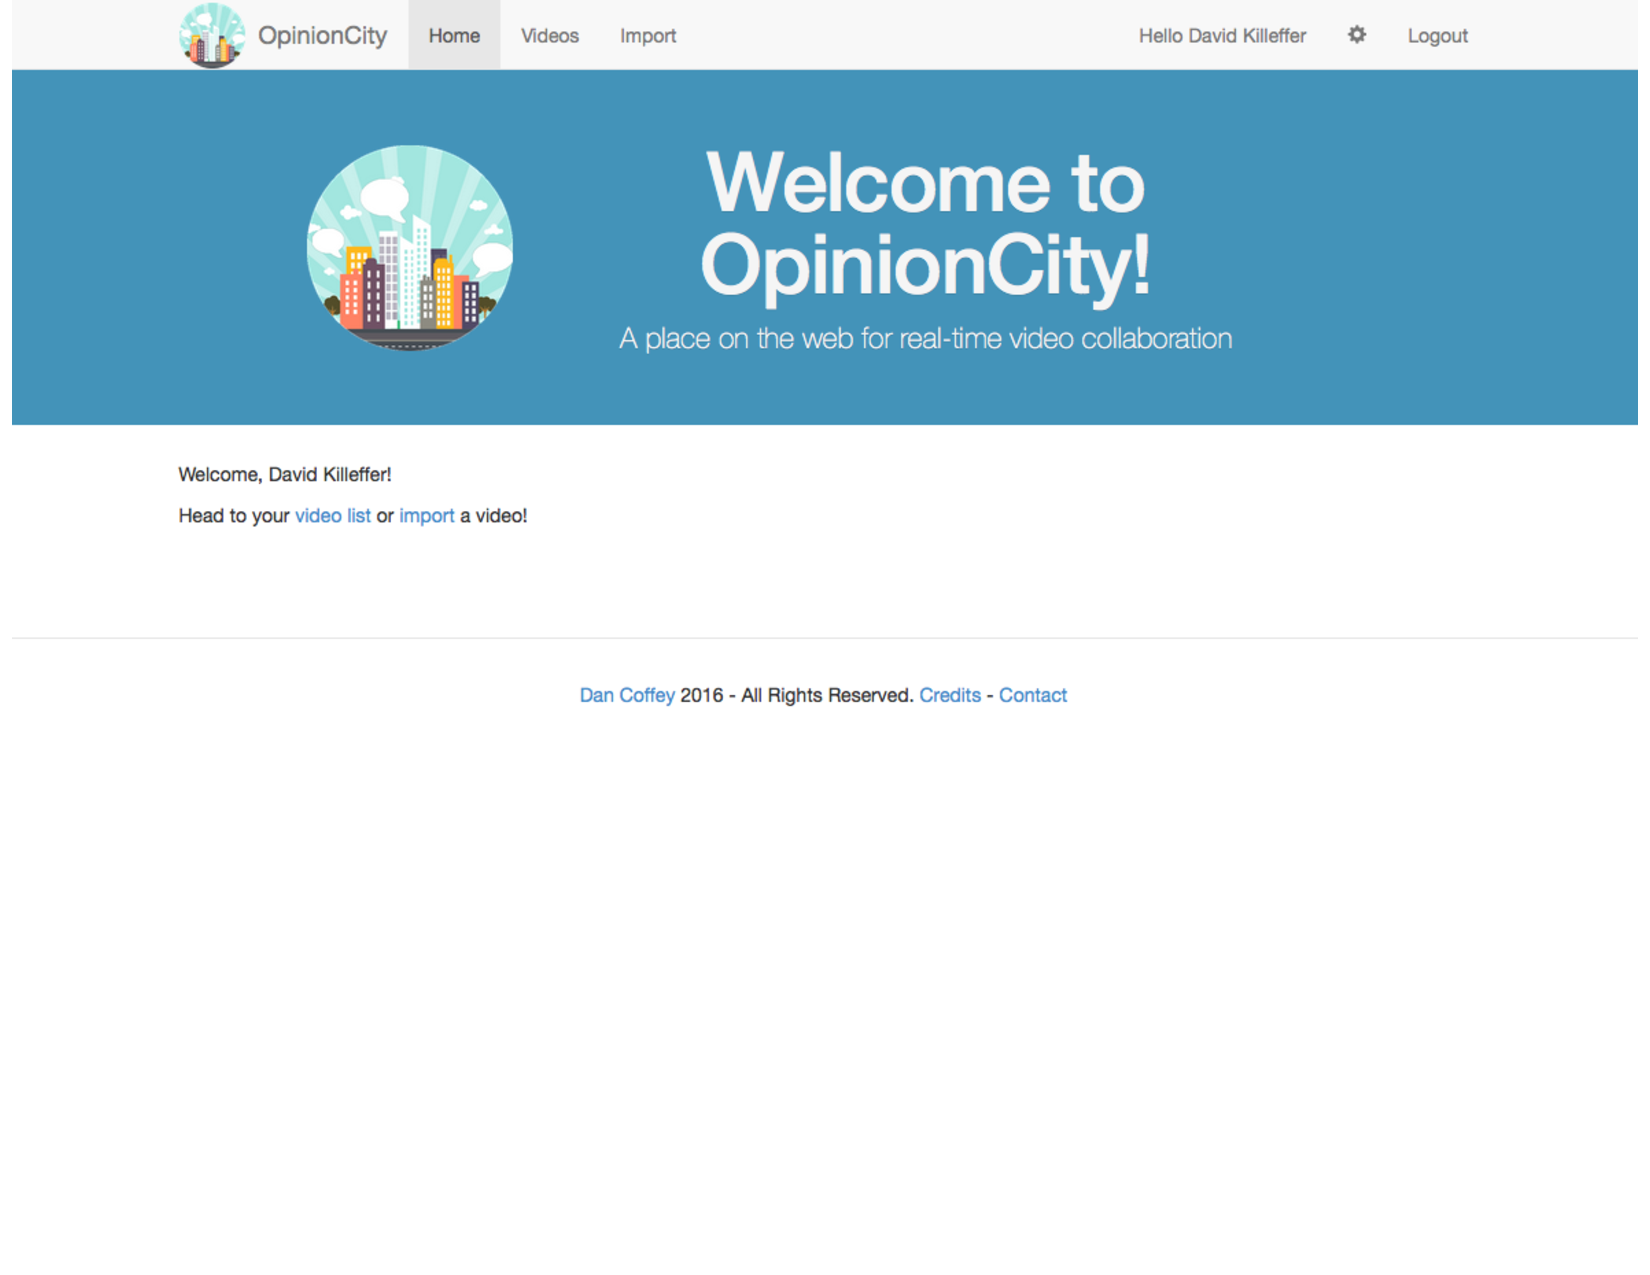
\includegraphics[width=\textwidth]{gfx/opinion-city/homepage1.pdf}
%	\caption{\textit{(OpinionCity)} homepage view} 
%	\label{fig:opinioncity:homepage-view}
%\end{figure} 

\begin{figure}[ht]
	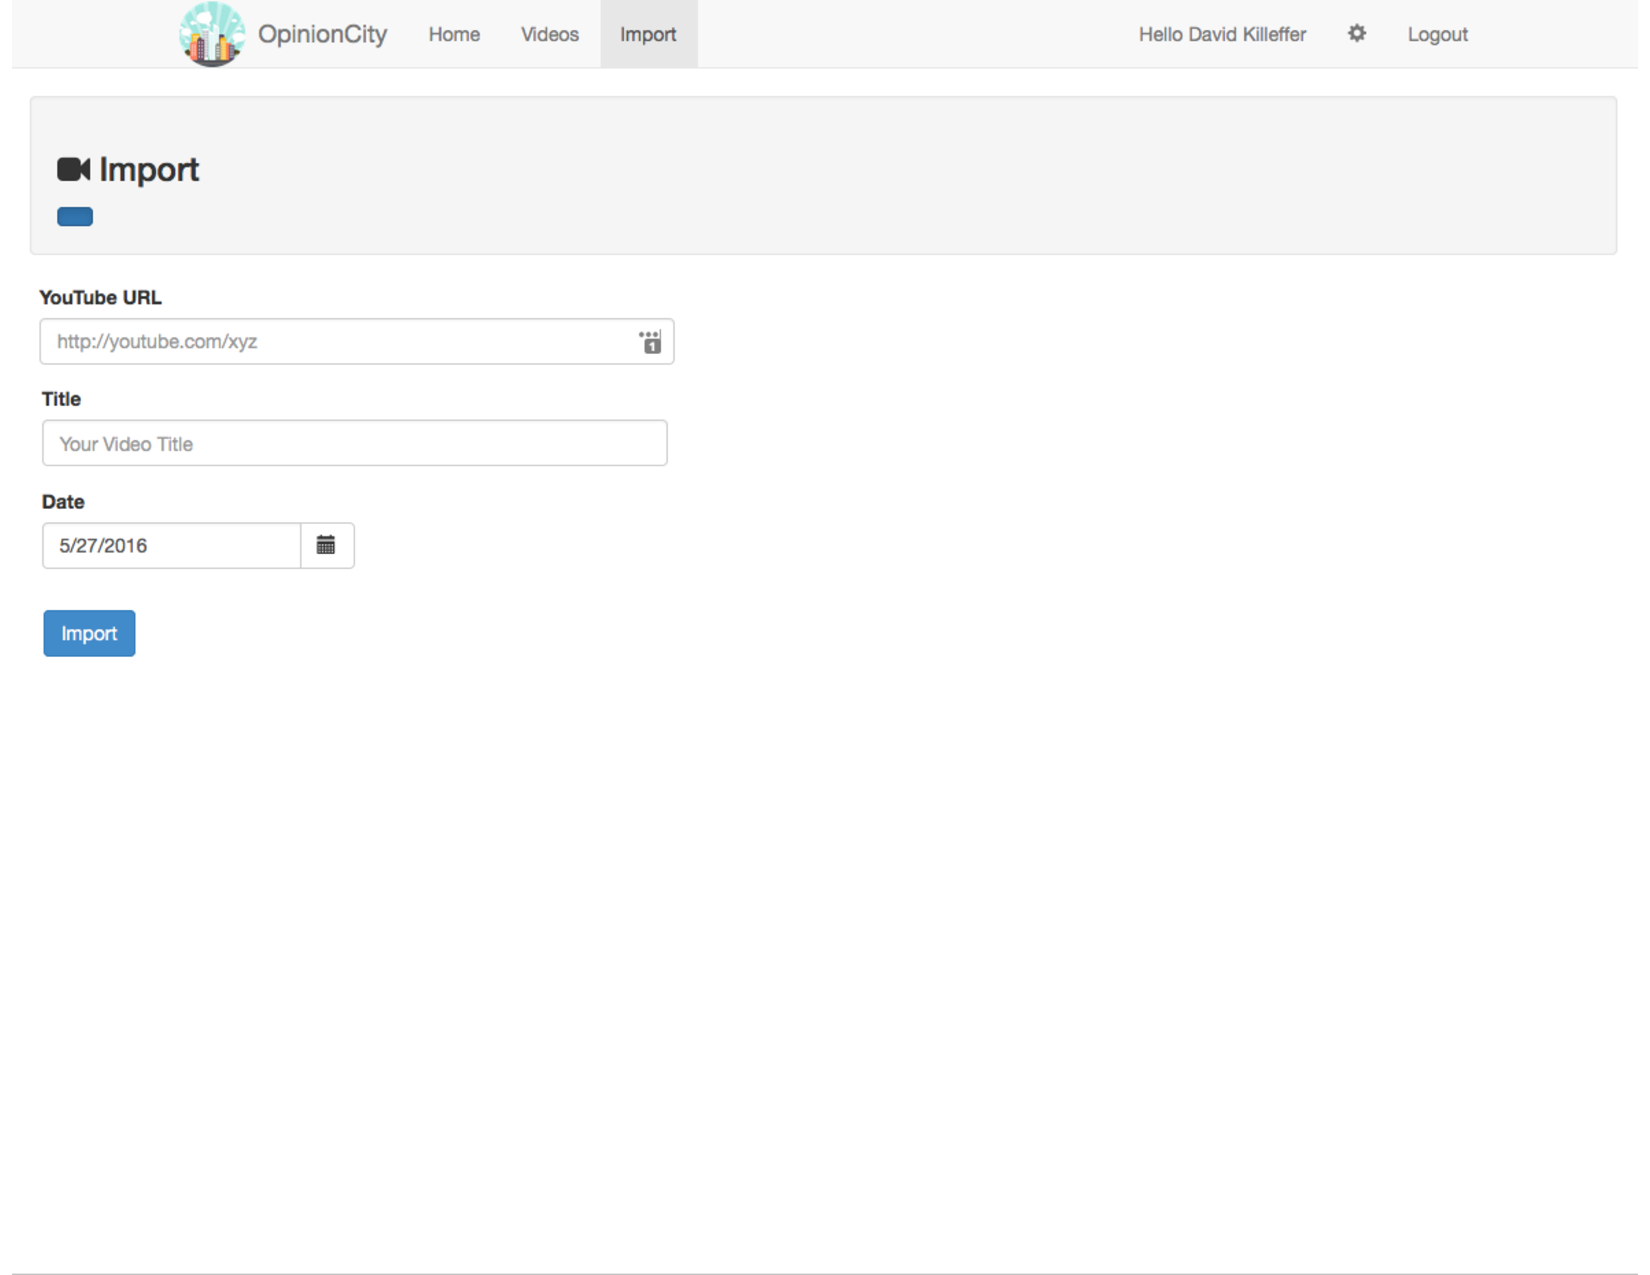
\includegraphics[width=\textwidth]{gfx/opinion-city/import1.pdf}
	\caption{\textit{(OpinionCity)} importing a video from \href{http://www.youtube.com}{YouTube} into OpinionCity} 
	\label{fig:opinioncity:importing-a-video-from-youtube}
\end{figure} 

\begin{figure}[ht]
	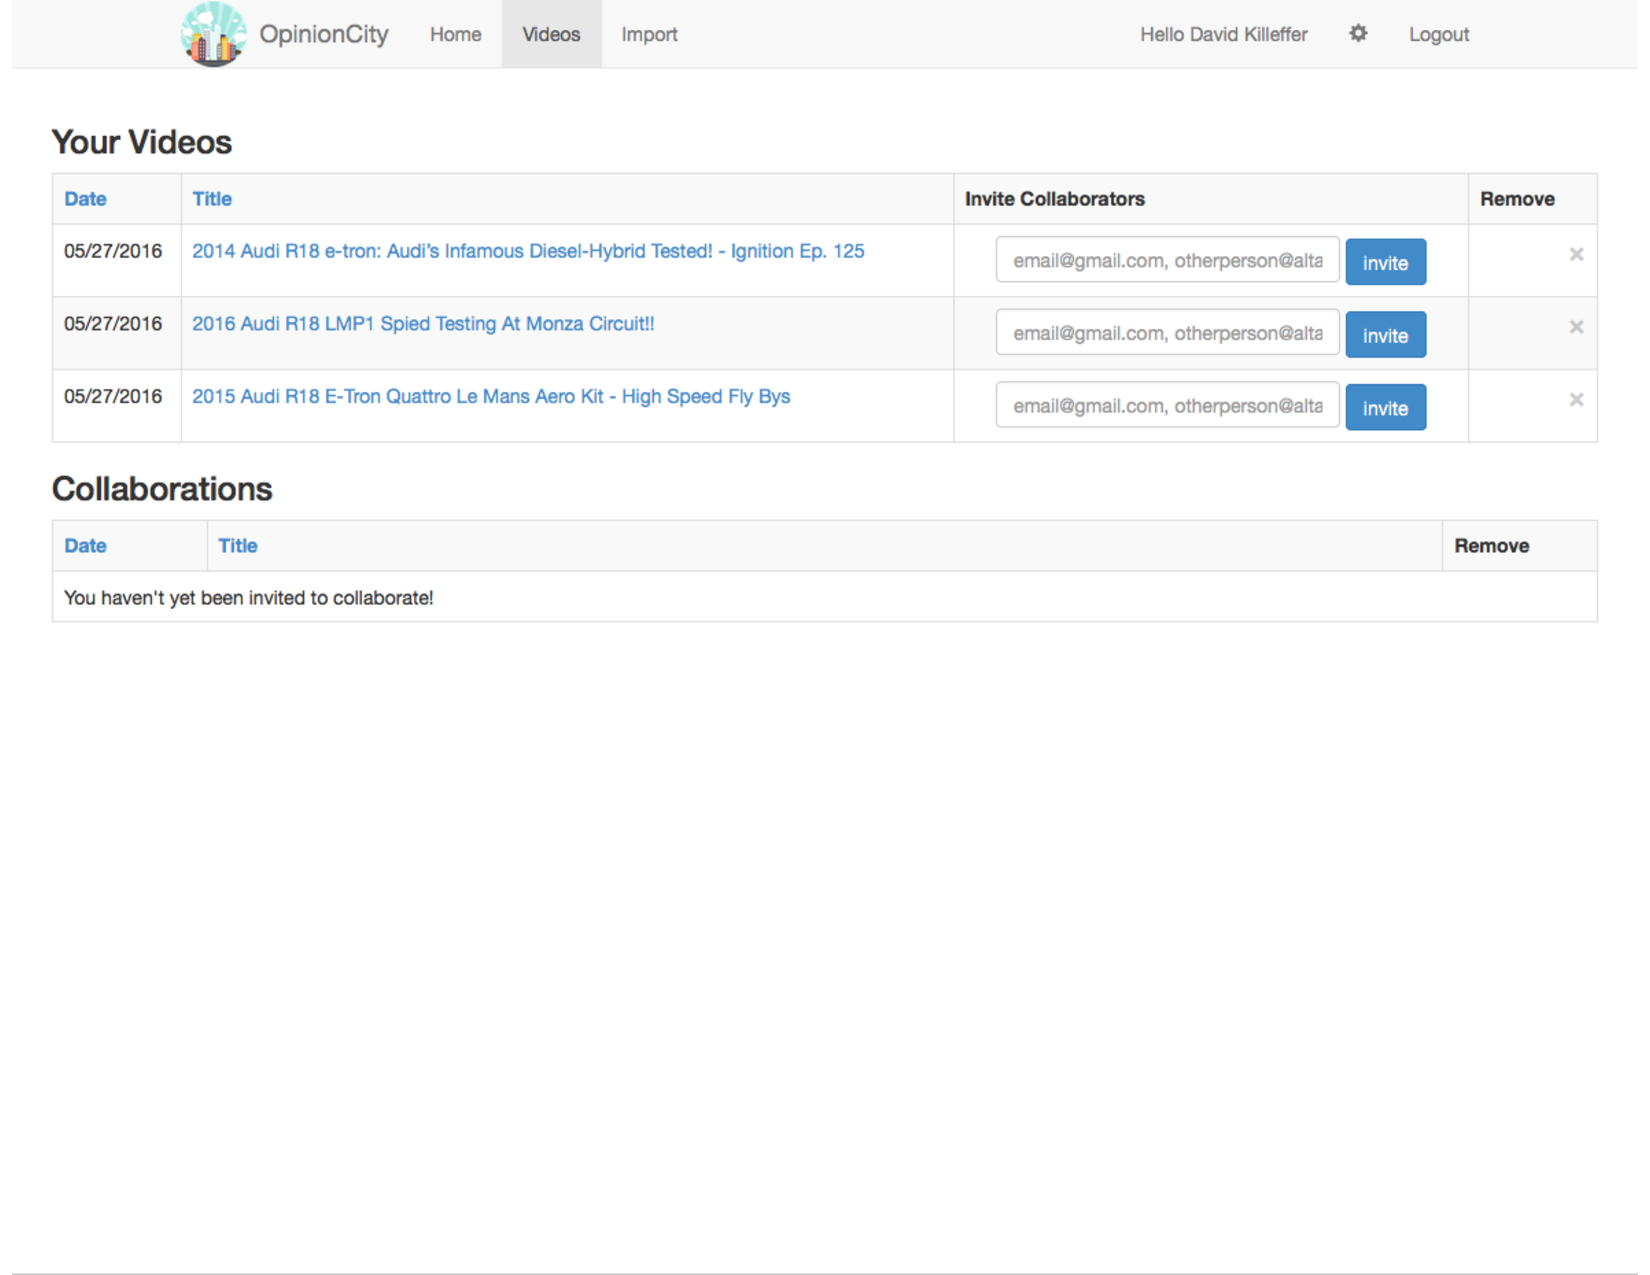
\includegraphics[width=\textwidth]{gfx/opinion-city/videolist1.pdf}
	\caption{\textit{(OpinionCity)} listing of all videos associated with a user account} 
	\label{fig:opinioncity:video-listing}
\end{figure}

%\begin{figure}[!ht]
%	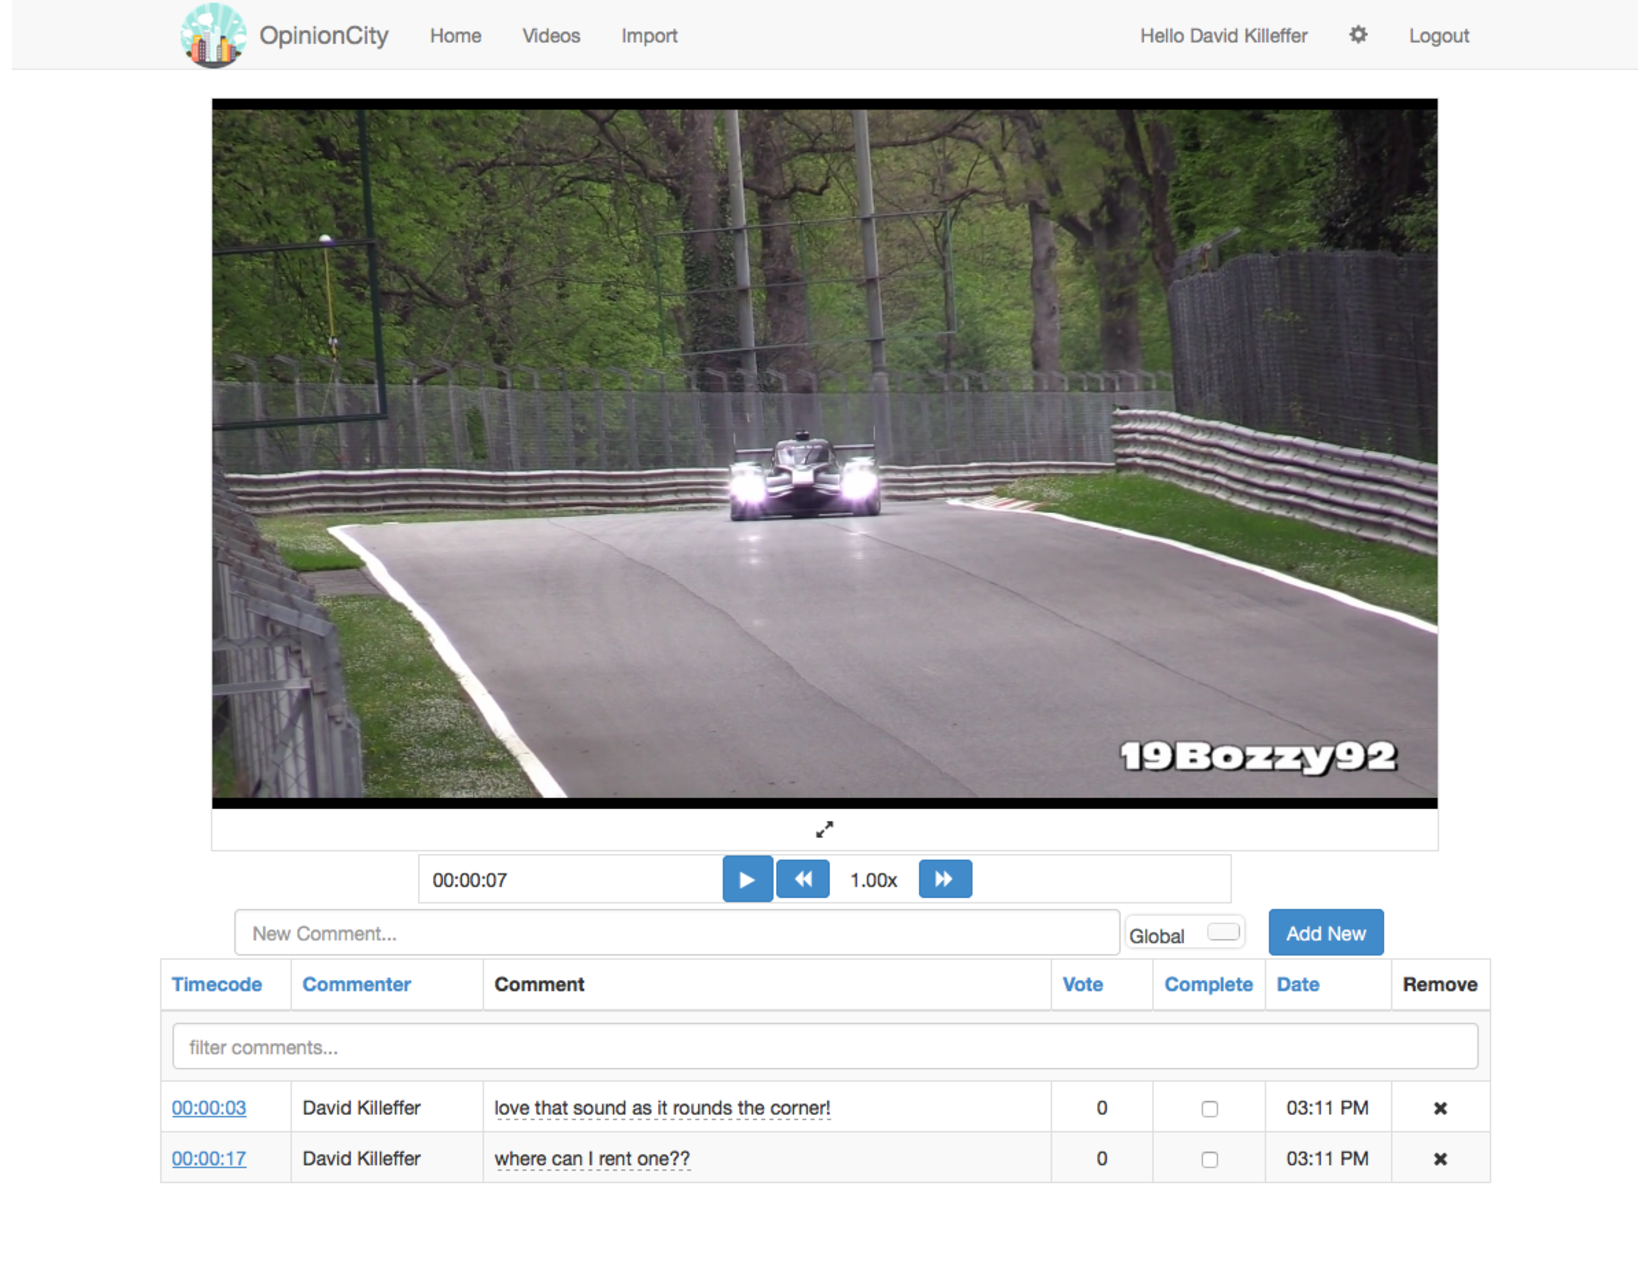
\includegraphics[width=\textwidth]{gfx/opinion-city/car1.pdf}
%	\caption{\textit{(OpinionCity)} adding video annotations} 
%	\label{fig:opinioncity:adding-video-annotations-view1}
%\end{figure}

\begin{figure}[ht]
	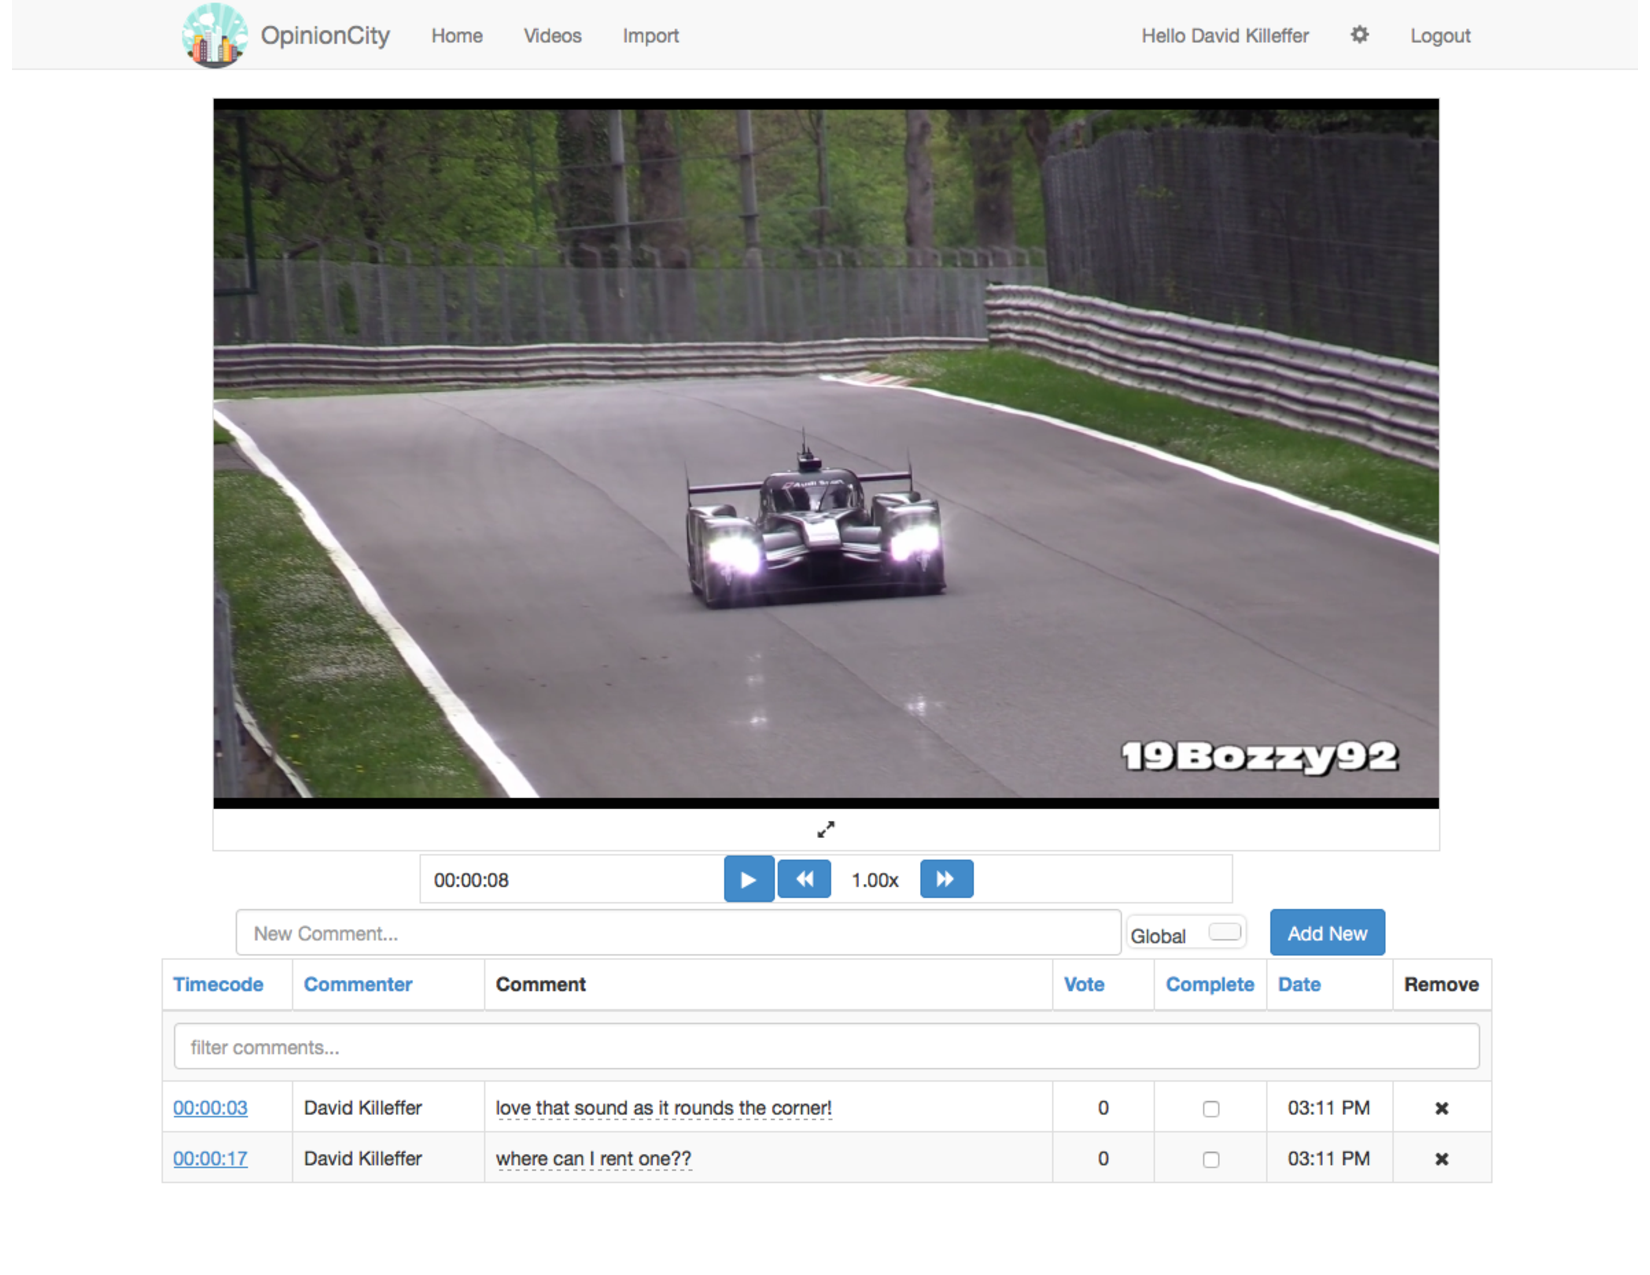
\includegraphics[width=\textwidth]{gfx/opinion-city/car2.pdf}
	\caption{\textit{(OpinionCity)} another view of adding video annotations} 
	\label{fig:opinioncity:adding-video-annotations-view2}
\end{figure}

\href{http://opinion.city}{OpinionCity} is a website that was created by Daniel P. Coffey for a Digital Media Capstone project at Harvard Extension School.  It is a tool for real-time group feedback on videos that have been uploaded to YouTube and allows for collaborative, time-code based annotation of videos as well as whole-video annotations.  Users may select a video to "upload" to OpinionCity where the video from YouTube will play in an embedded player, and then users can add comments to the video at specific timecodes or apply their remarks to the entire video.  Users can also invite others to join in and comment on the video as well. 

While OpinionCity does allow for users to add annotations to specific parts of videos, it does not appear to allow for very granular annotations; specifically, a user may add an annotation at a specific part of the video denoting the "beginning" of an annotation, but cannot mark the "end" of the annotation.  This means that the annotation functionality is somewhat limited in that users are not able to define during what specific timeframe in a video a person is in, or where the video was shot, etc.  For annotating relatively shorter-length videos such as are often found on YouTube, this may be fine, but for annotating entire tape-length (typically 60-120 minutes or occasionally longer), this mechanism would be insufficient. 

Additionally, OpinionCity does not appear to have any search functionality.  Users may add annotations to videos, but there is no mechanism whereby they can then later search what annotations have been added.  The project seems to have focused much more on the real-time aspects of commenting on a video, where a group of interested people may be watching a video at the same time and then making annotations and comments, and quickly viewing what others have likewise annotated and commented.  Here are some screenshots of OpinionCity:

%\\ 
%{\centering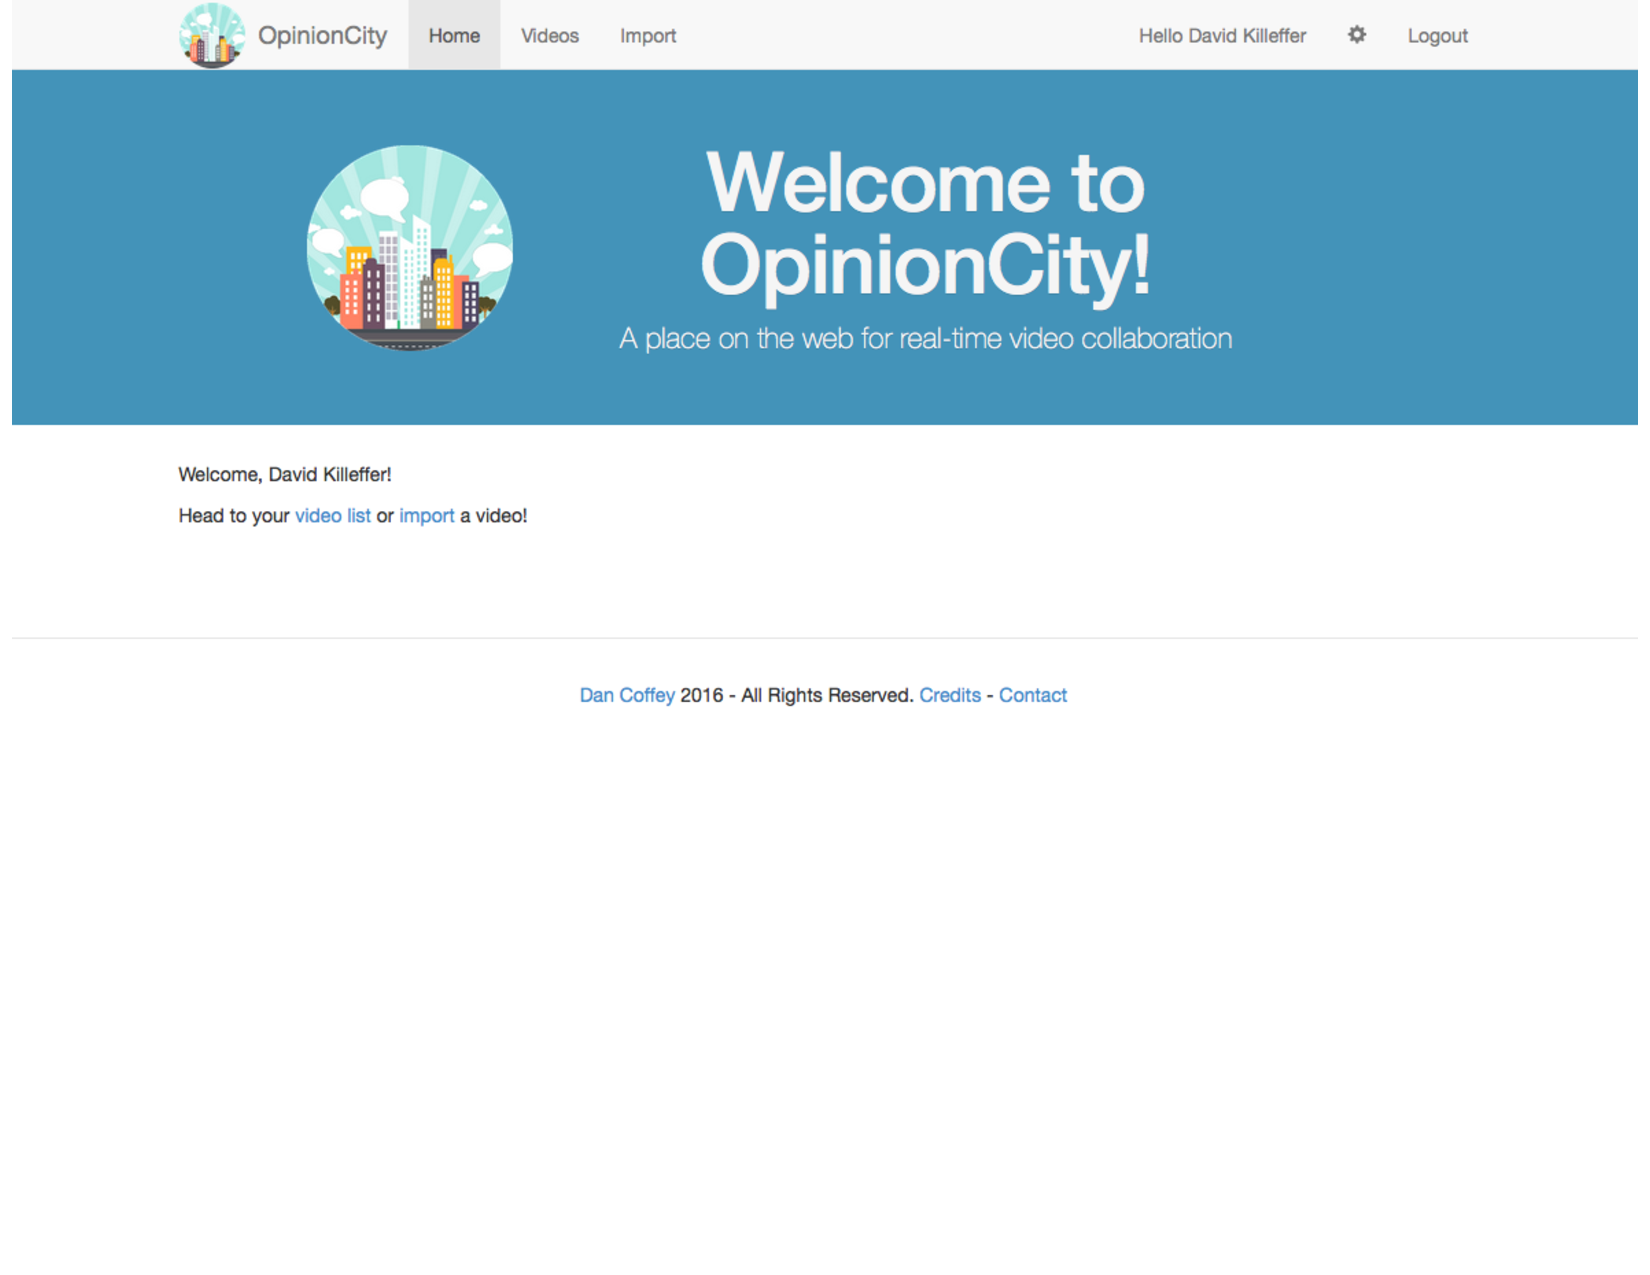
\includegraphics[width=1\textwidth]{gfx/opinion-city/homepage1.pdf}} \\
%{\centering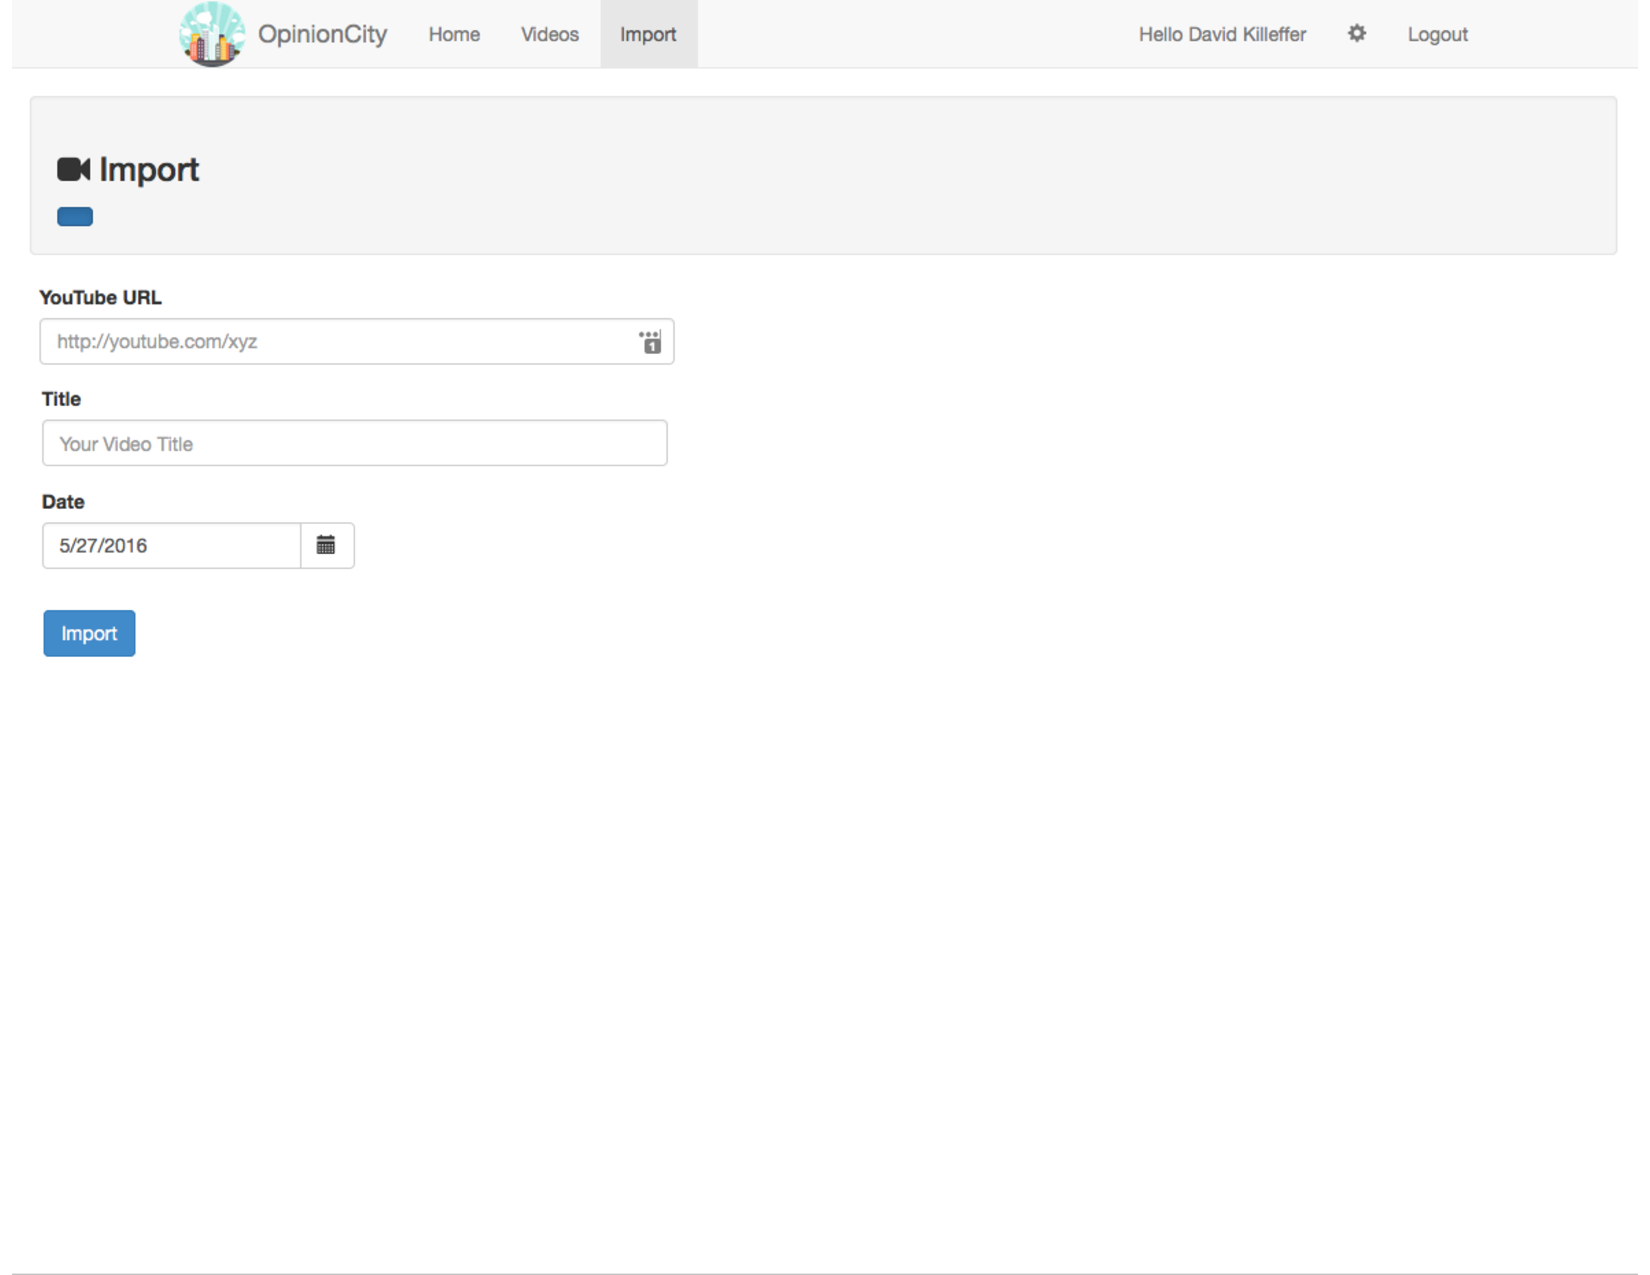
\includegraphics[width=1\textwidth]{gfx/opinion-city/import1.pdf}} \\
%{\centering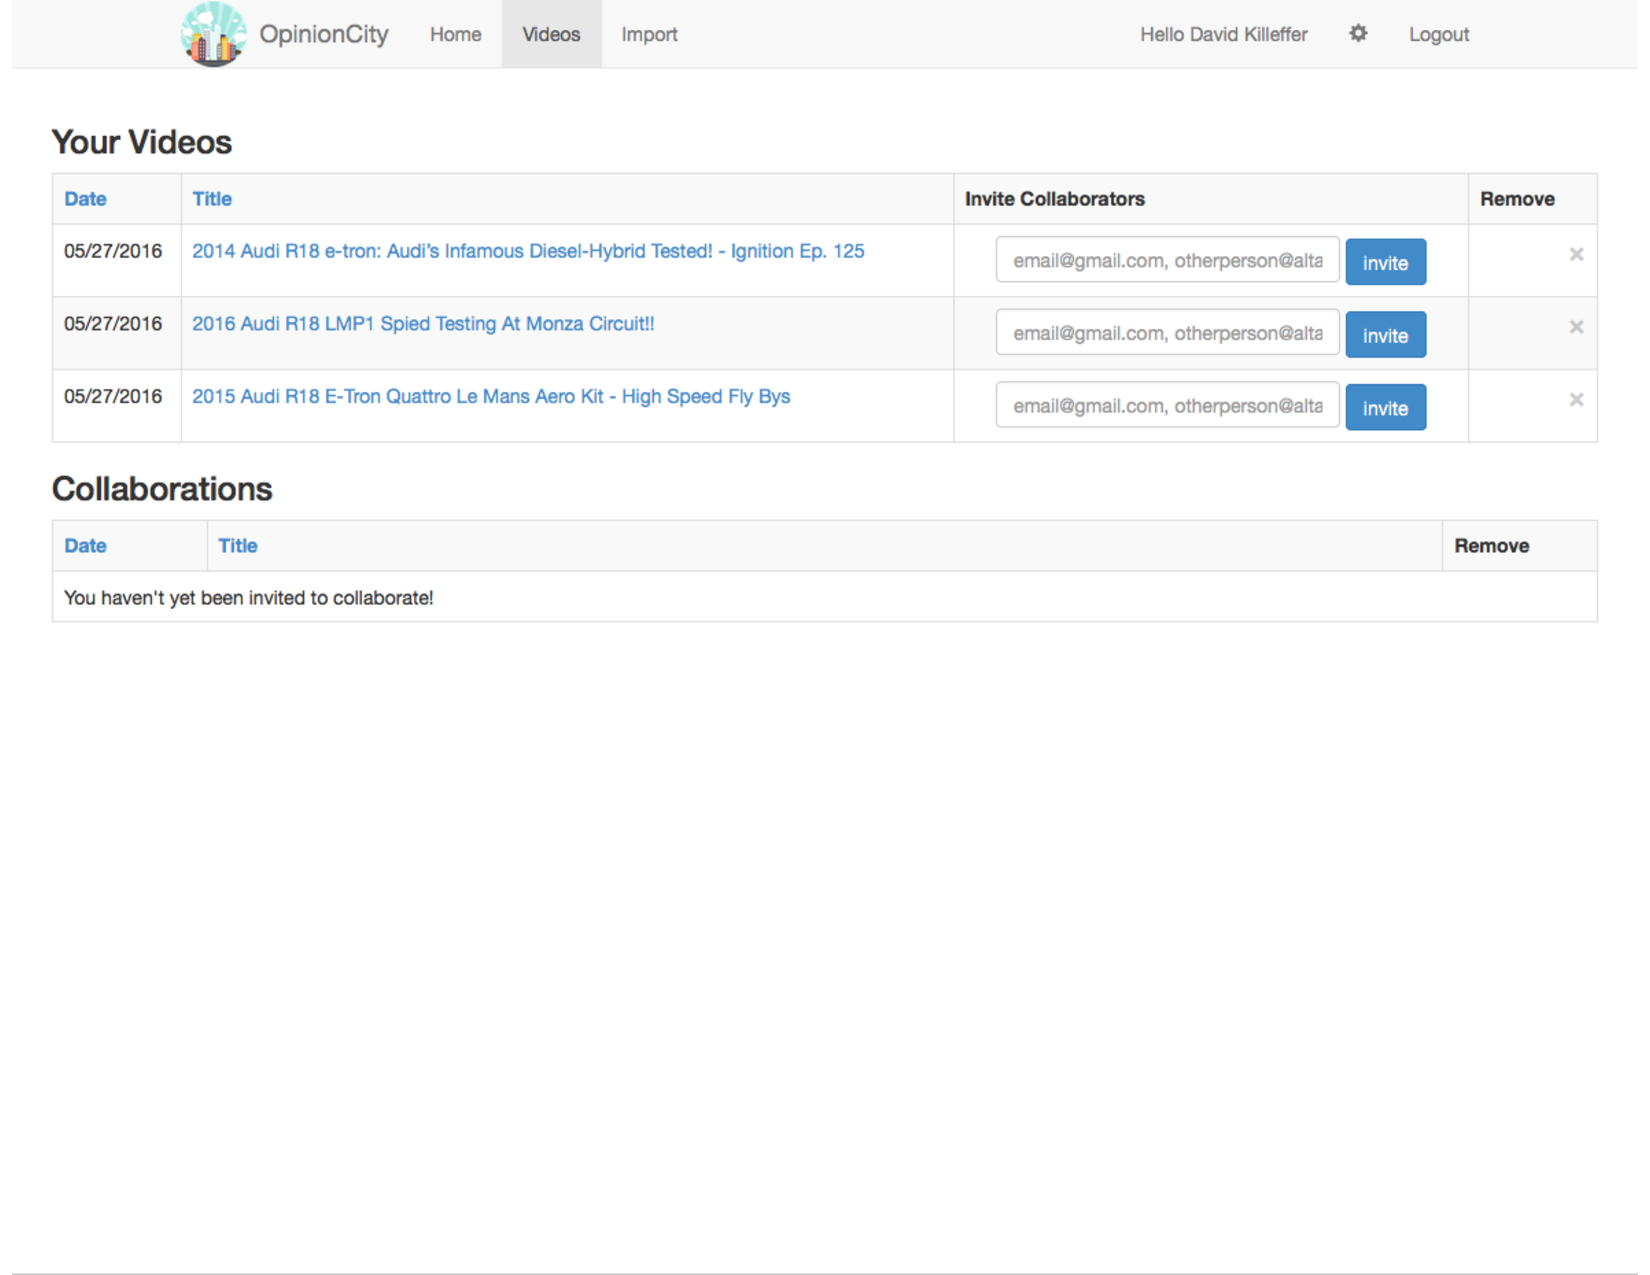
\includegraphics[width=1\textwidth]{gfx/opinion-city/videolist1.pdf}} \\
%{\centering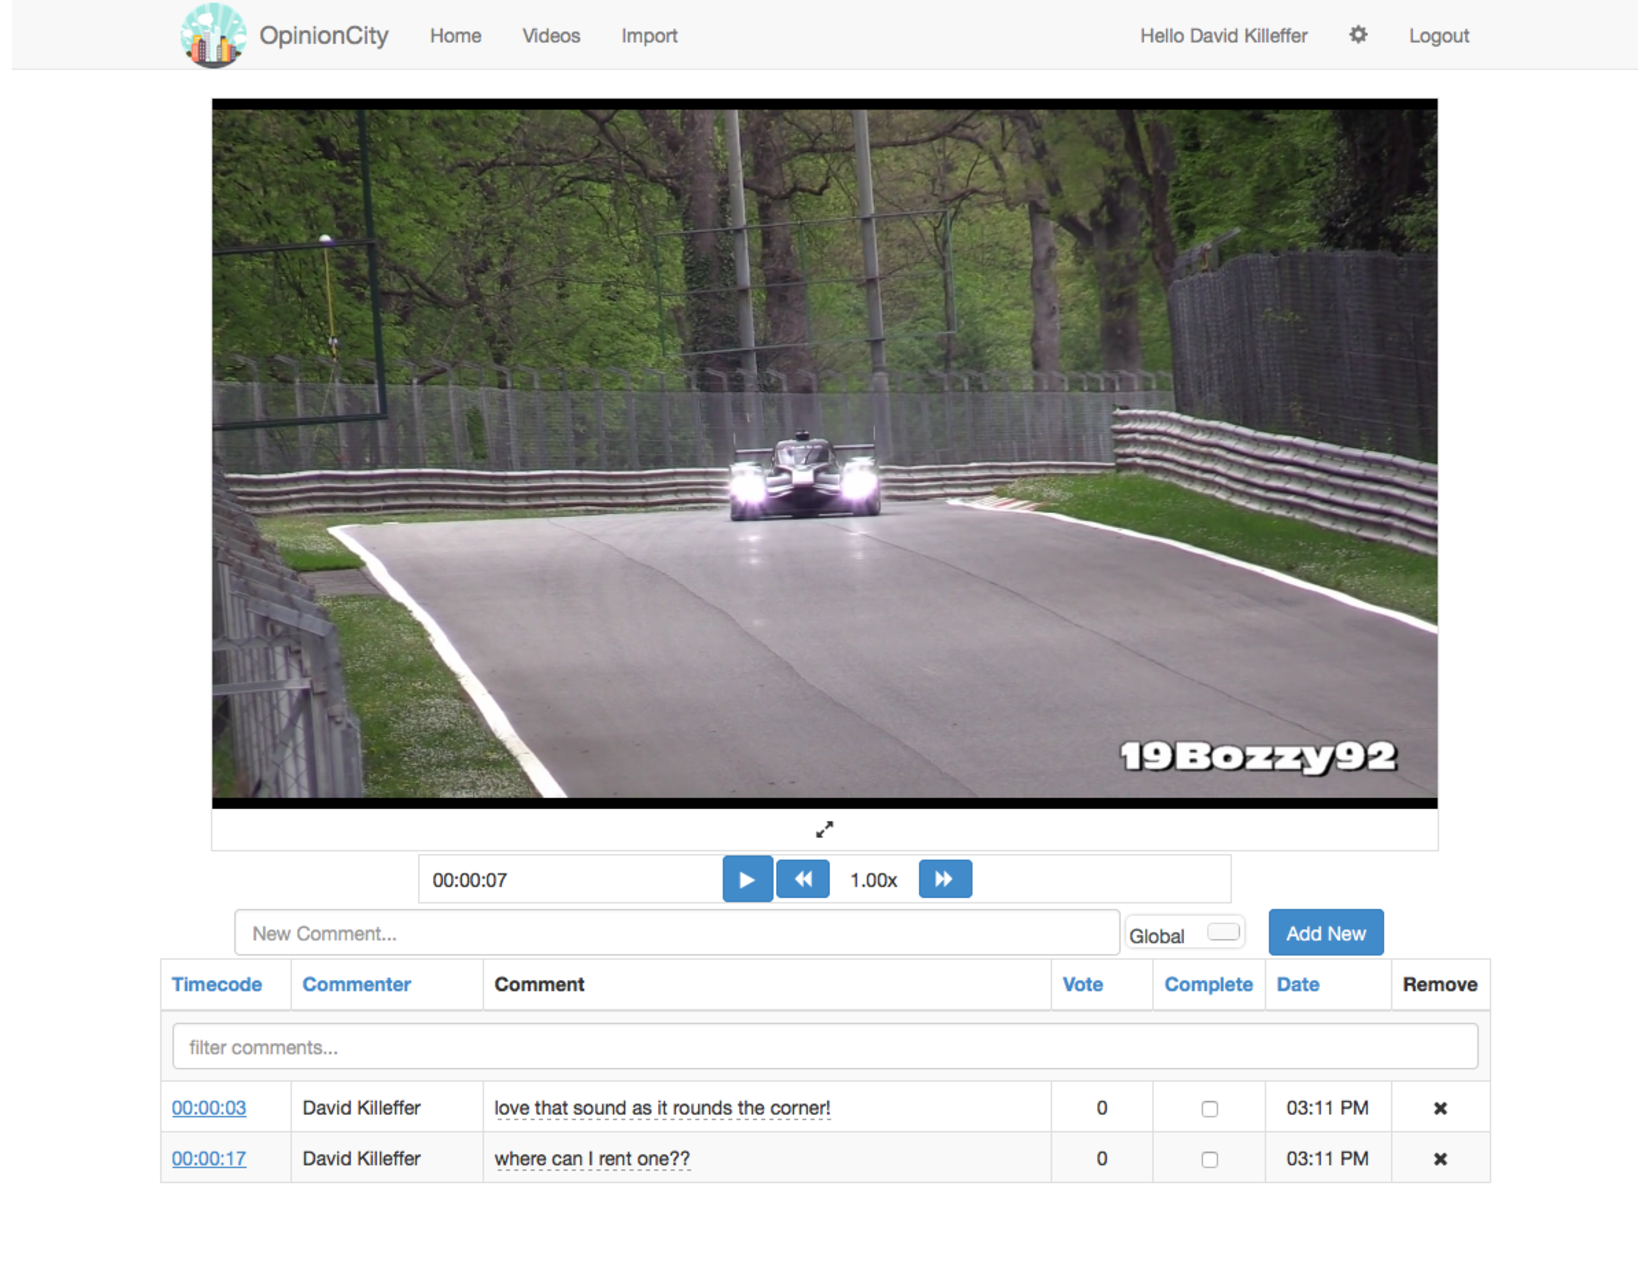
\includegraphics[width=1\textwidth]{gfx/opinion-city/car1.pdf}} \\
%{\centering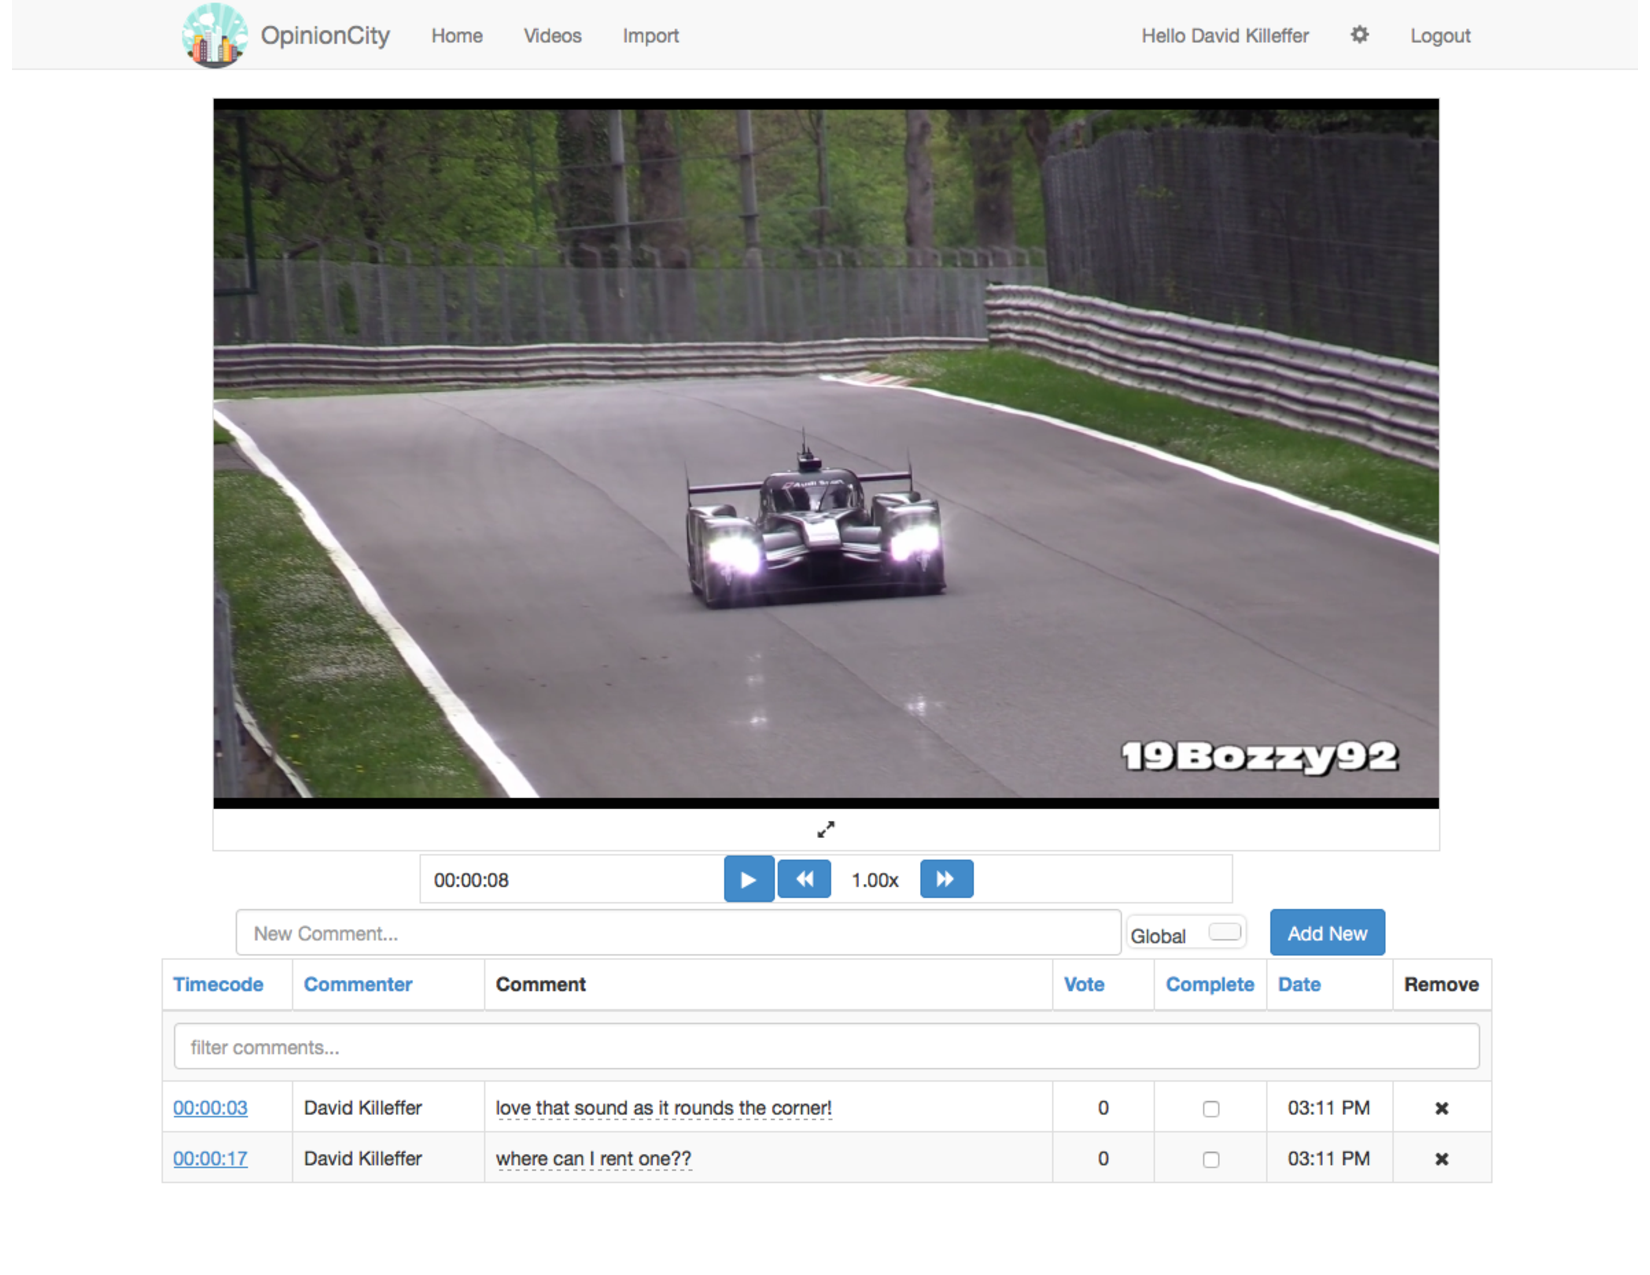
\includegraphics[width=1\textwidth]{gfx/opinion-city/car2.pdf}} \\

%{\centering
%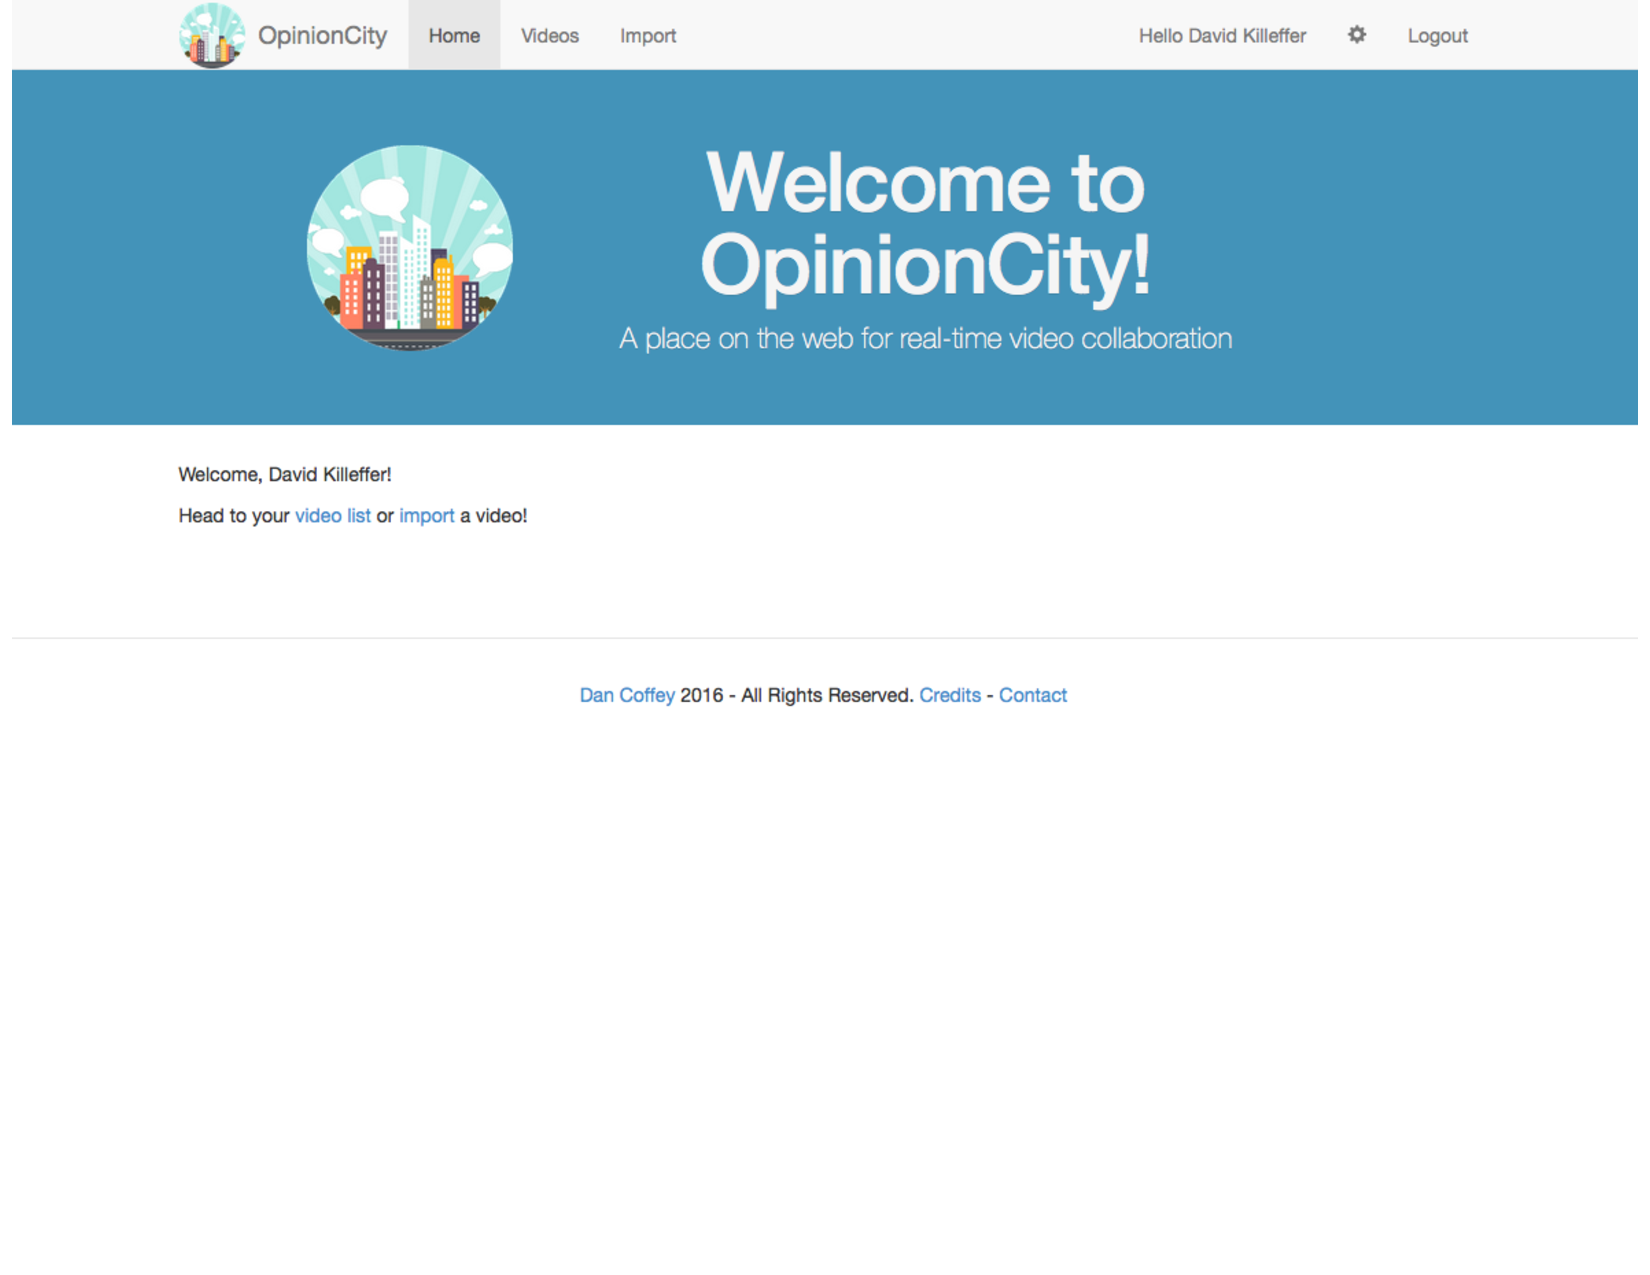
\includegraphics[width=1\textwidth]{gfx/opinion-city/homepage1.pdf} \\
%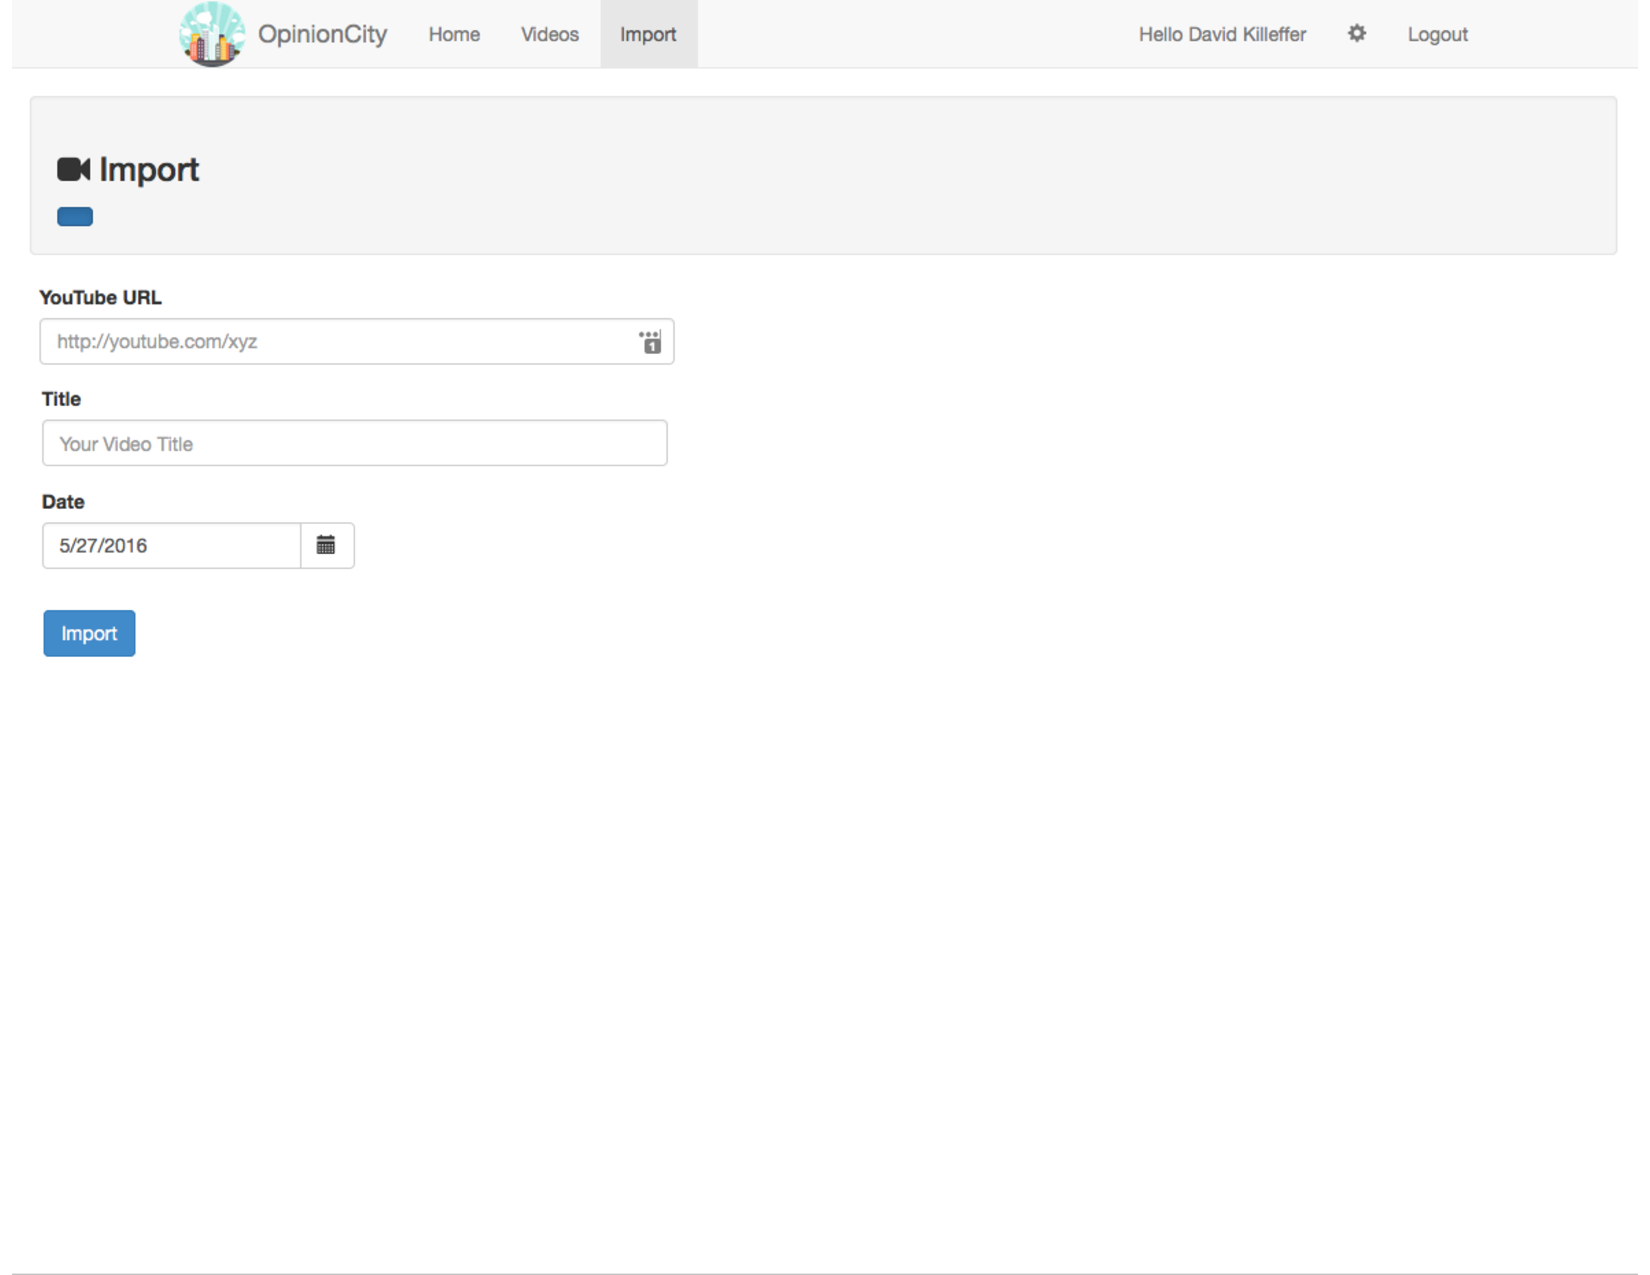
\includegraphics[width=1\textwidth]{gfx/opinion-city/import1.pdf} \\
%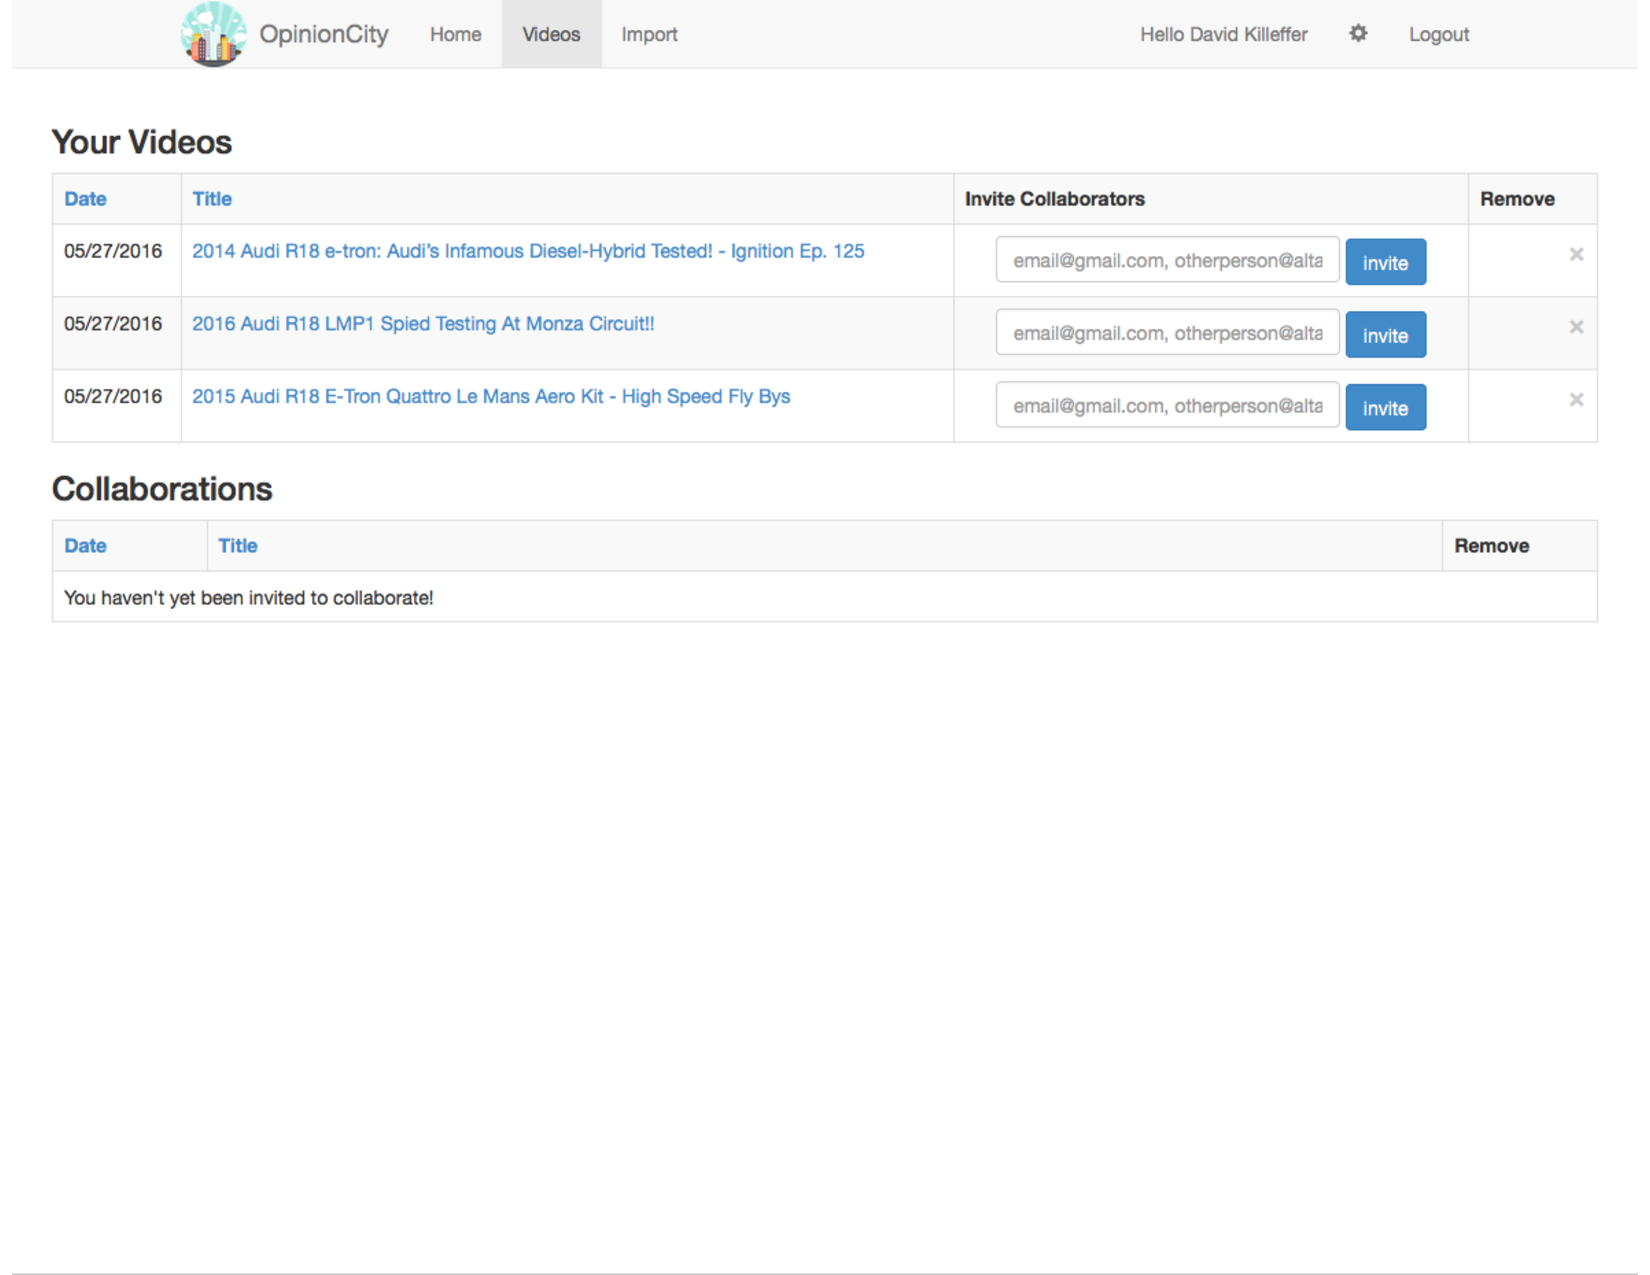
\includegraphics[width=1\textwidth]{gfx/opinion-city/videolist1.pdf} \\
%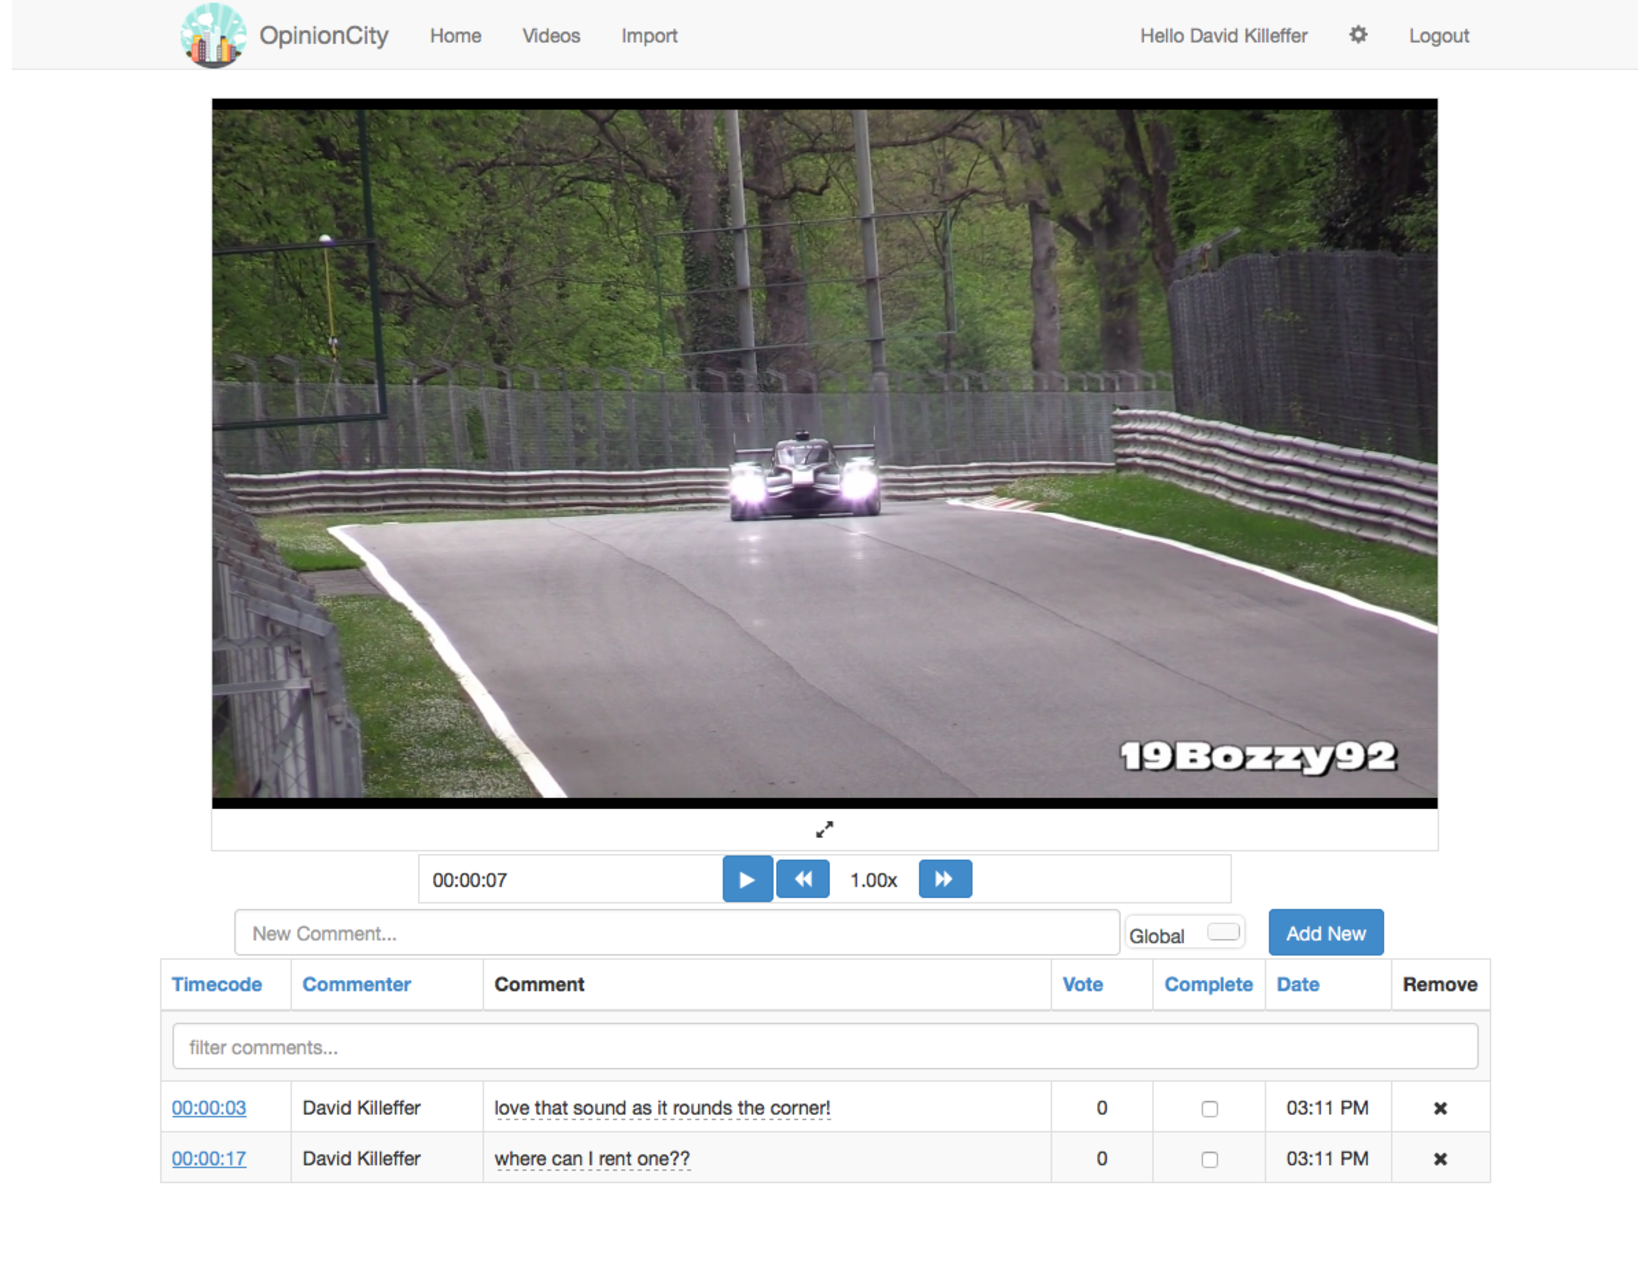
\includegraphics[width=1\textwidth]{gfx/opinion-city/car1.pdf} \\
%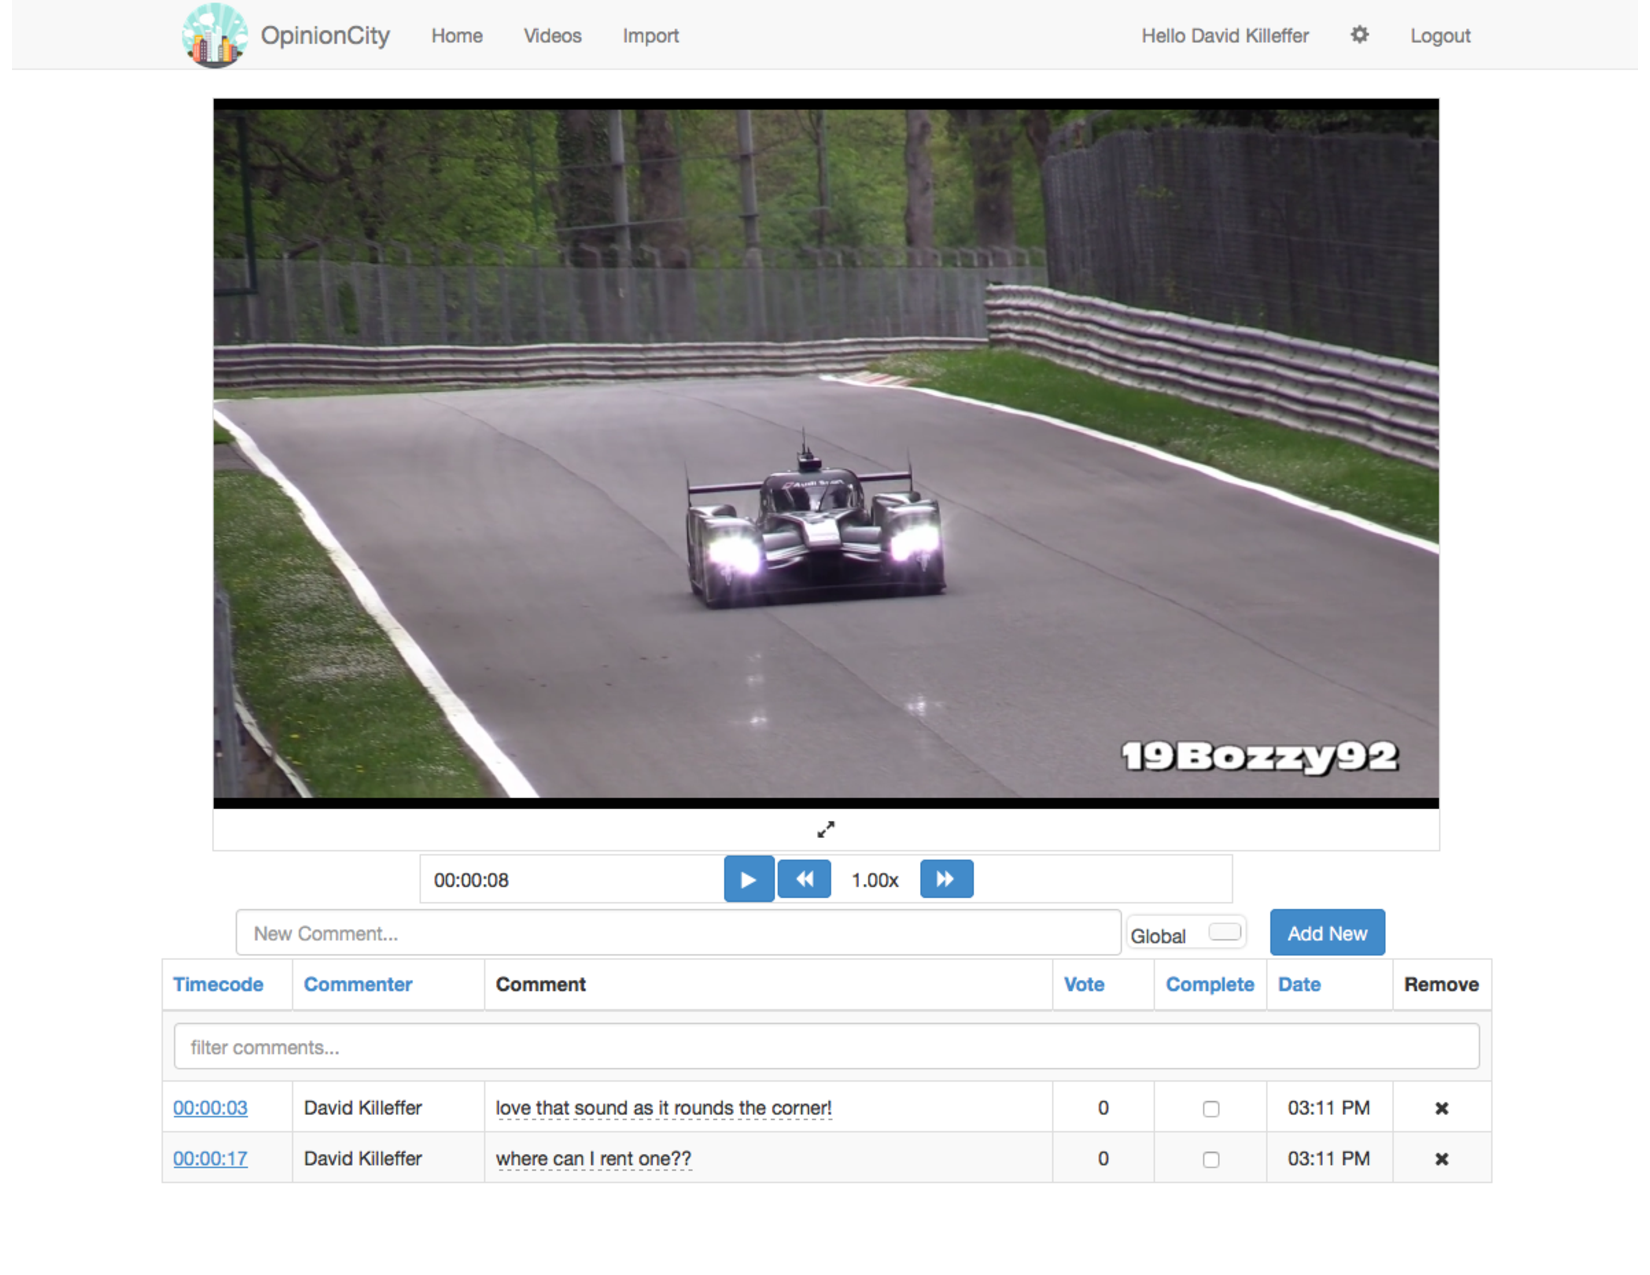
\includegraphics[width=1\textwidth]{gfx/opinion-city/car2.pdf} \\
%}


\section{Media-rich Video Annotation Tool (MVAT)}
\label{sec:priorwork:media-rich-video-annotation-tool}

%\item \textit{Media-rich Video Annotation Tool (MVAT)}, by Philip Desenne: \href{mailto:desenne@fas.harvard.edu}{\nolinkurl{desenne@fas.harvard.edu} }, May 2012 \\
%\textit{Media-rich Video Annotation Tool (MVAT)}, by Philip Desenne: \href{mailto:desenne@fas.harvard.edu}{\nolinkurl{desenne@fas.harvard.edu} }, May 2012
\textit{by Philip Desenne: \href{mailto:desenne@fas.harvard.edu}{\nolinkurl{desenne@fas.harvard.edu} }, May 2012}

\begin{figure}[!ht]
	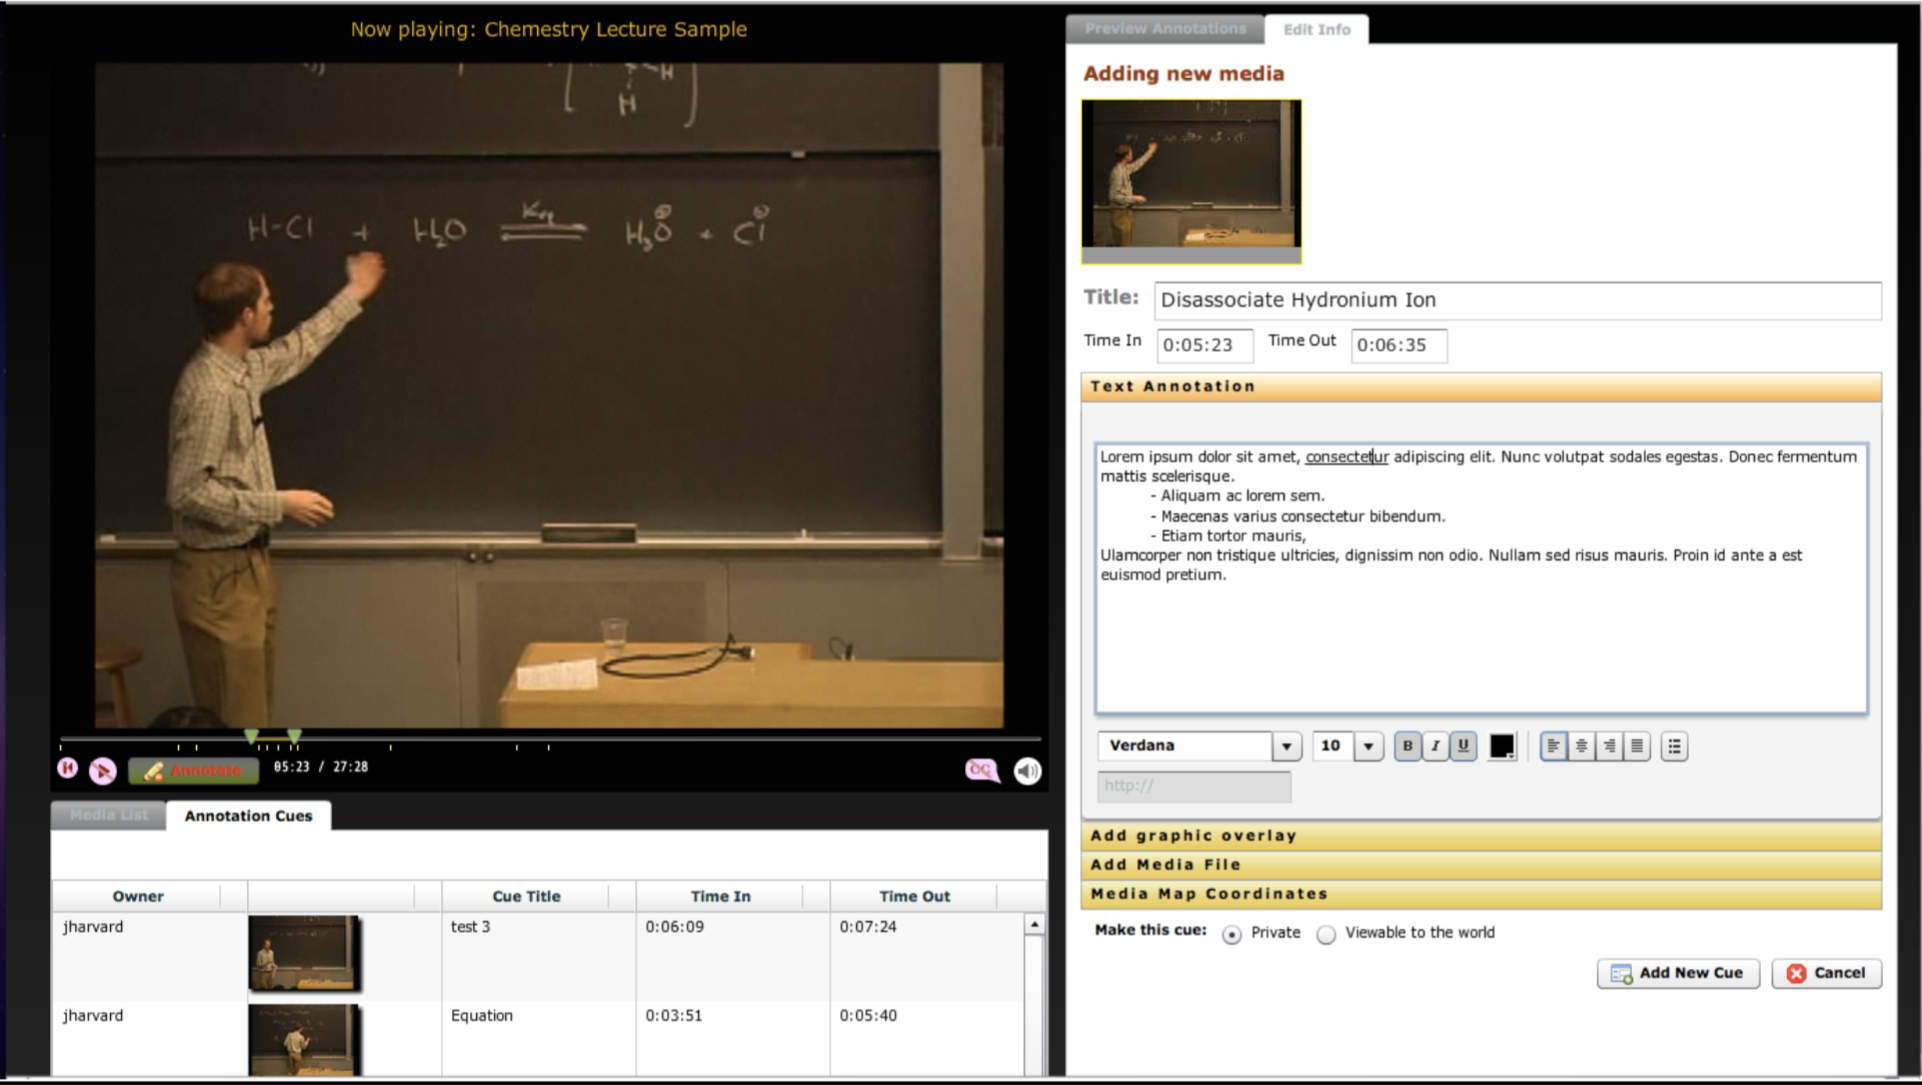
\includegraphics[width=\textwidth]{gfx/mvat/mvat-annotation-edit-view.png}
	\caption{\textit{(MVAT)} video annotation edit view} 
	\label{fig:mvat:video-annotation-edit-view}
\end{figure} 

\begin{figure}[!ht]
	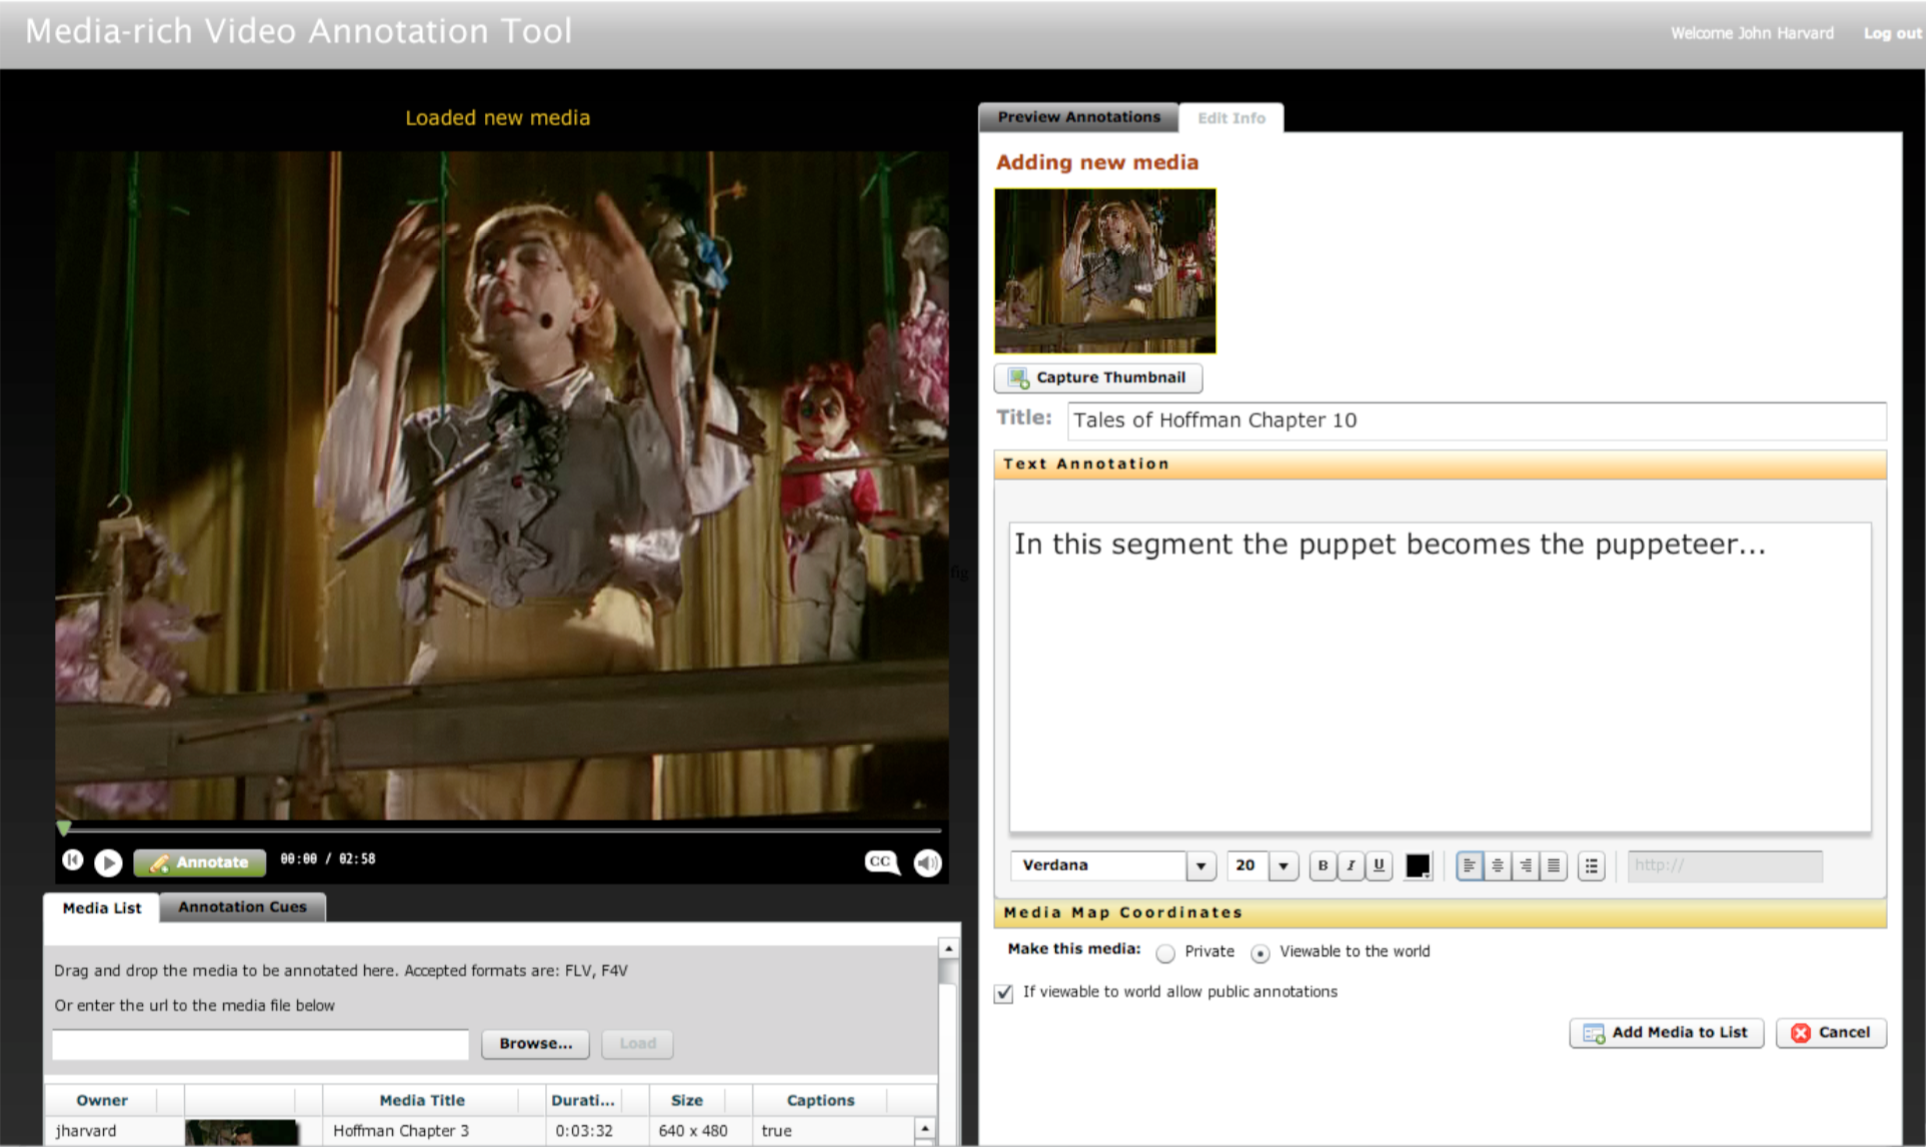
\includegraphics[width=\textwidth]{gfx/mvat/mvat-loading-video-adding-metadata.png}
	\caption{\textit{(MVAT)} adding video metadata view} 
	\label{fig:mvat:adding-video-metadata}
\end{figure} 

\begin{figure}[!ht]
	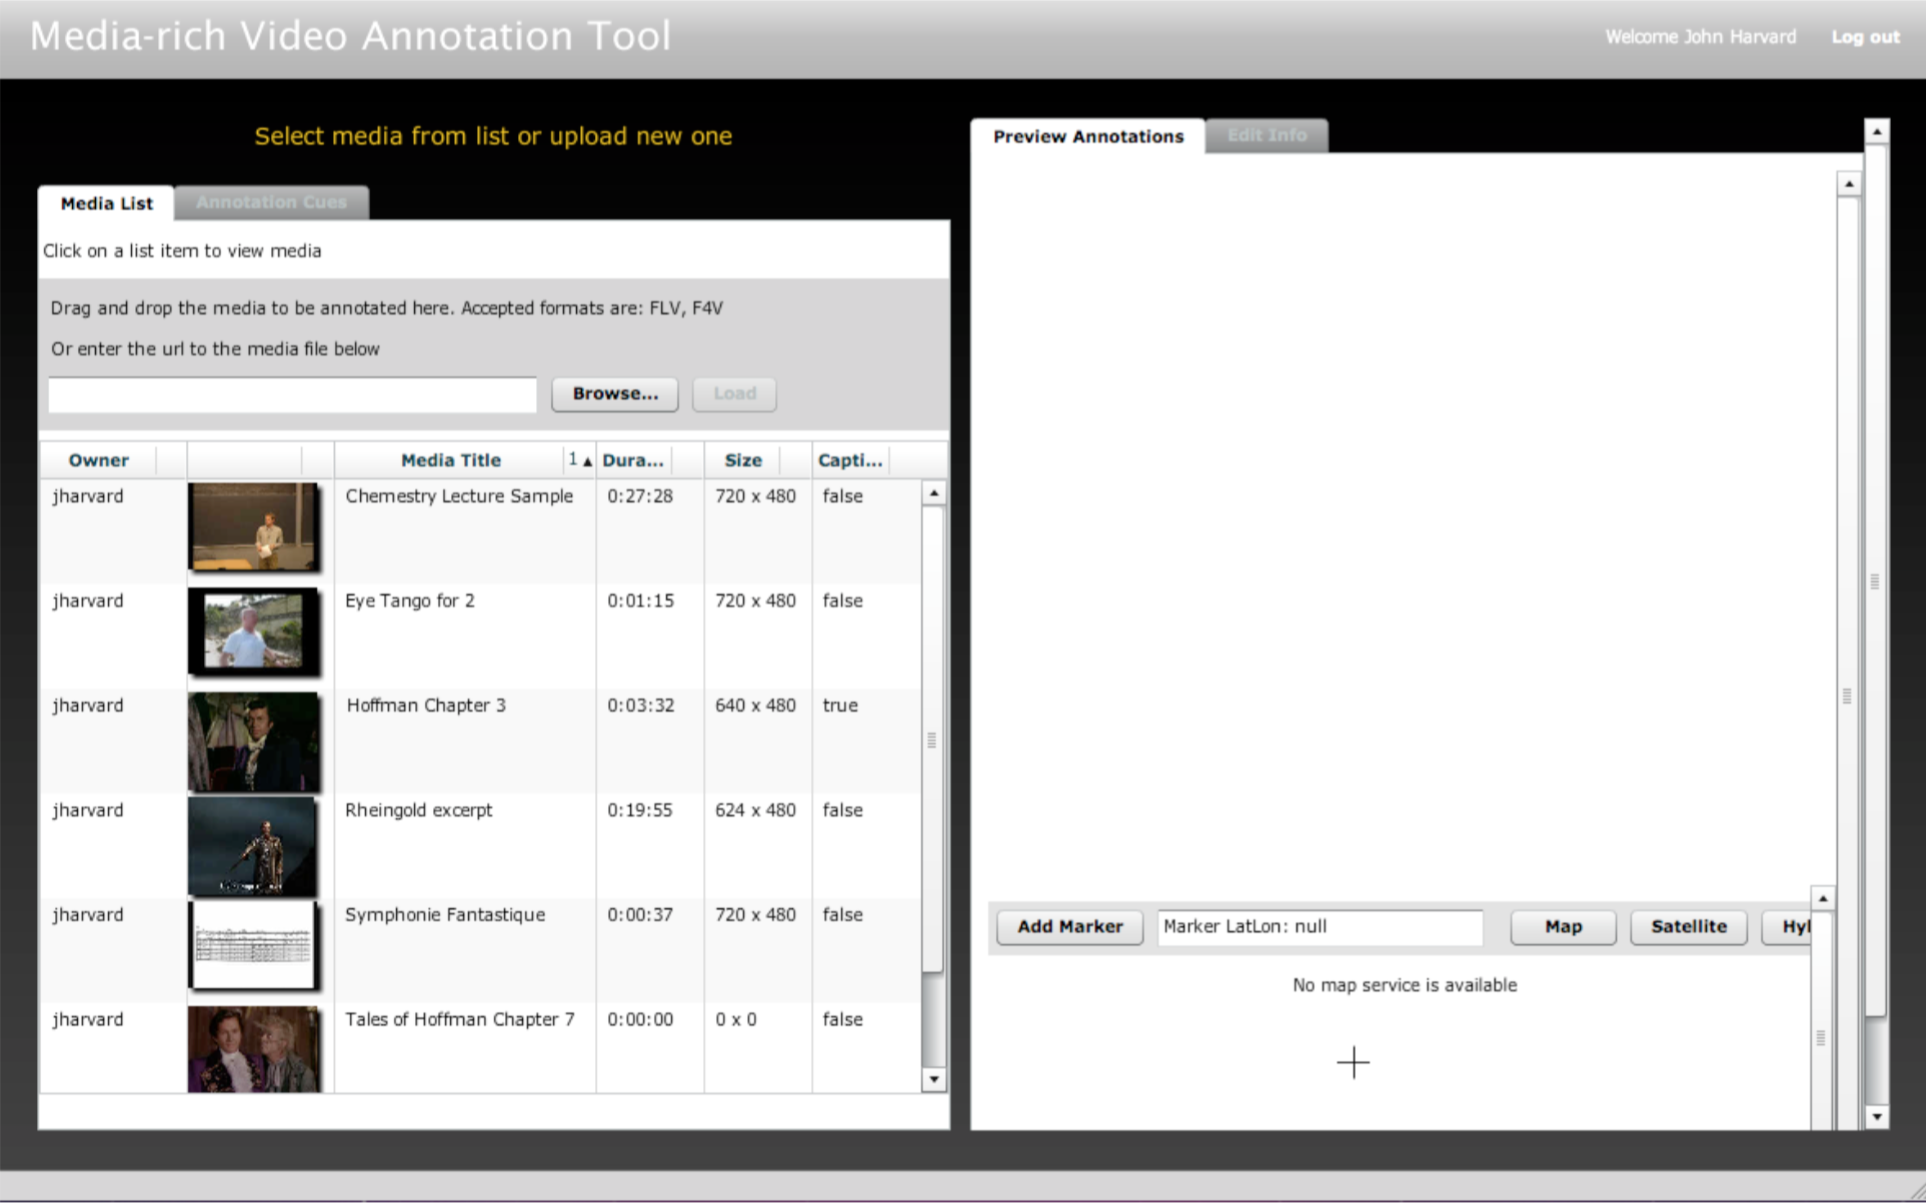
\includegraphics[width=\textwidth]{gfx/mvat/mvat-video-management}
	\caption{\textit{(MVAT)} video management view} 
	\label{fig:mvat:video-management-view}
\end{figure}

The Media-rich Video Annotation Tool (MVAT) is a prototype tool developed by Philip Desenne as part of an A.L.M. in Information Technology thesis project at Harvard Extension School.  Motivation for the development of the MVAT stemmed from Desenne's work as an Academic Technologies Product Manager to support learning and simplify the process of creating and sharing video annotations amongst students in a pedagogical context.  MVAT allows for a wide variety of media rich annotations, including adding text, HTML, pictures, actual vector drawings that users add, geographical notations, etc., all of which are very useful and support the educational aims of lecture videos.

The prototype focused on allowing users to create "media-rich" annotations so users could add much more than just plain text or image annotations, as well as link to outside supporting resources, and have a very simple, easy-to-use interface.  MVAT was developed as an Adobe Air standalone application, and requires a data synchronization mechanism to upload annotations to an online SQL database from the embedded SQL-Lite database.  Desenne acknowledged that while his selection of Adobe Air / Flex as a development platform enabled him to rapidly prototype the MVAT due to his experience with Adobe Air / Flex, it is a rather limiting choice long-term since Flex "was unleashed from Adobe" and Flash video usage has largely gone to the wayside in favor of open standards for video such as HTML5 video.  Additionally, the MVAT prototype was limited to a single computer, and so other students were not able to benefit from, search for, or share the annotations made by one user with other classmates.
%\\ 
%Here are some screenshots of MVAT: \\

%{\centering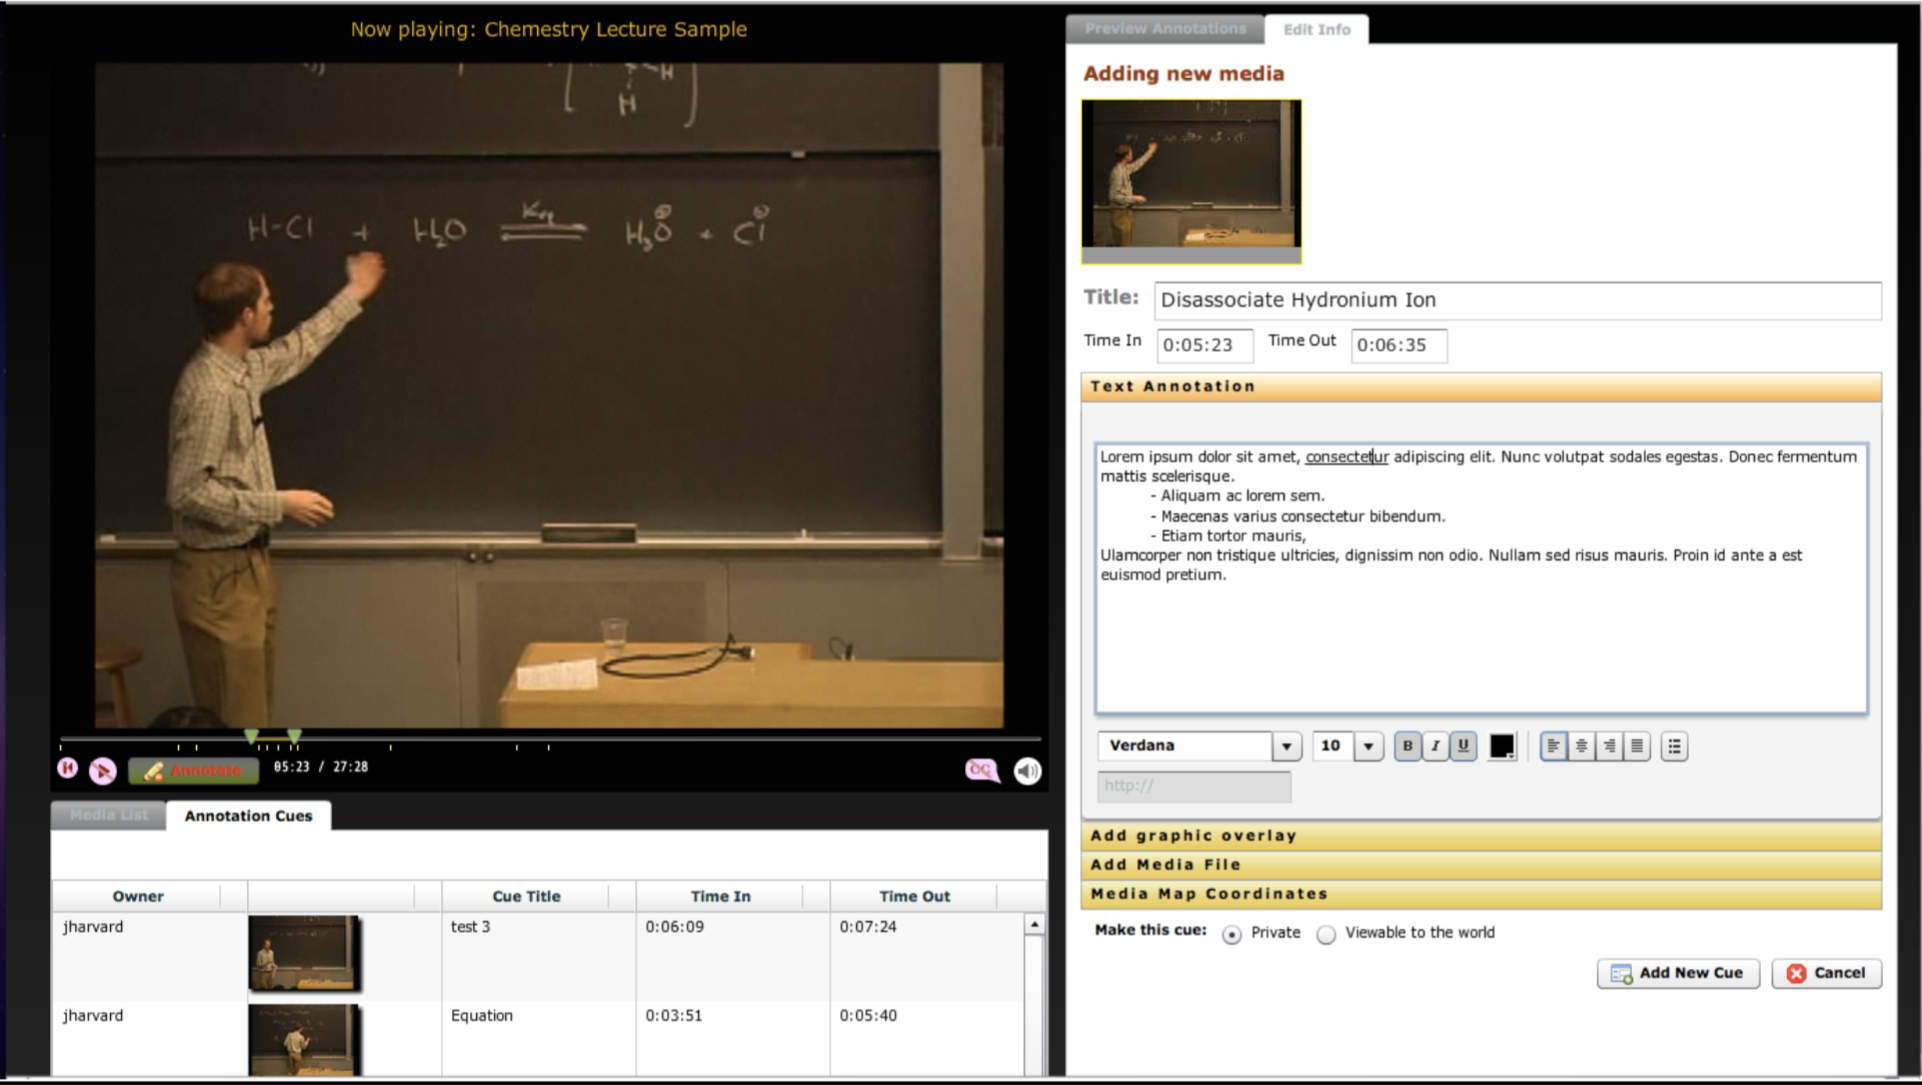
\includegraphics[width=1\textwidth]{gfx/mvat/mvat-annotation-edit-view.png}} \\
%{\centering

%\begin{figure}[htb]
%	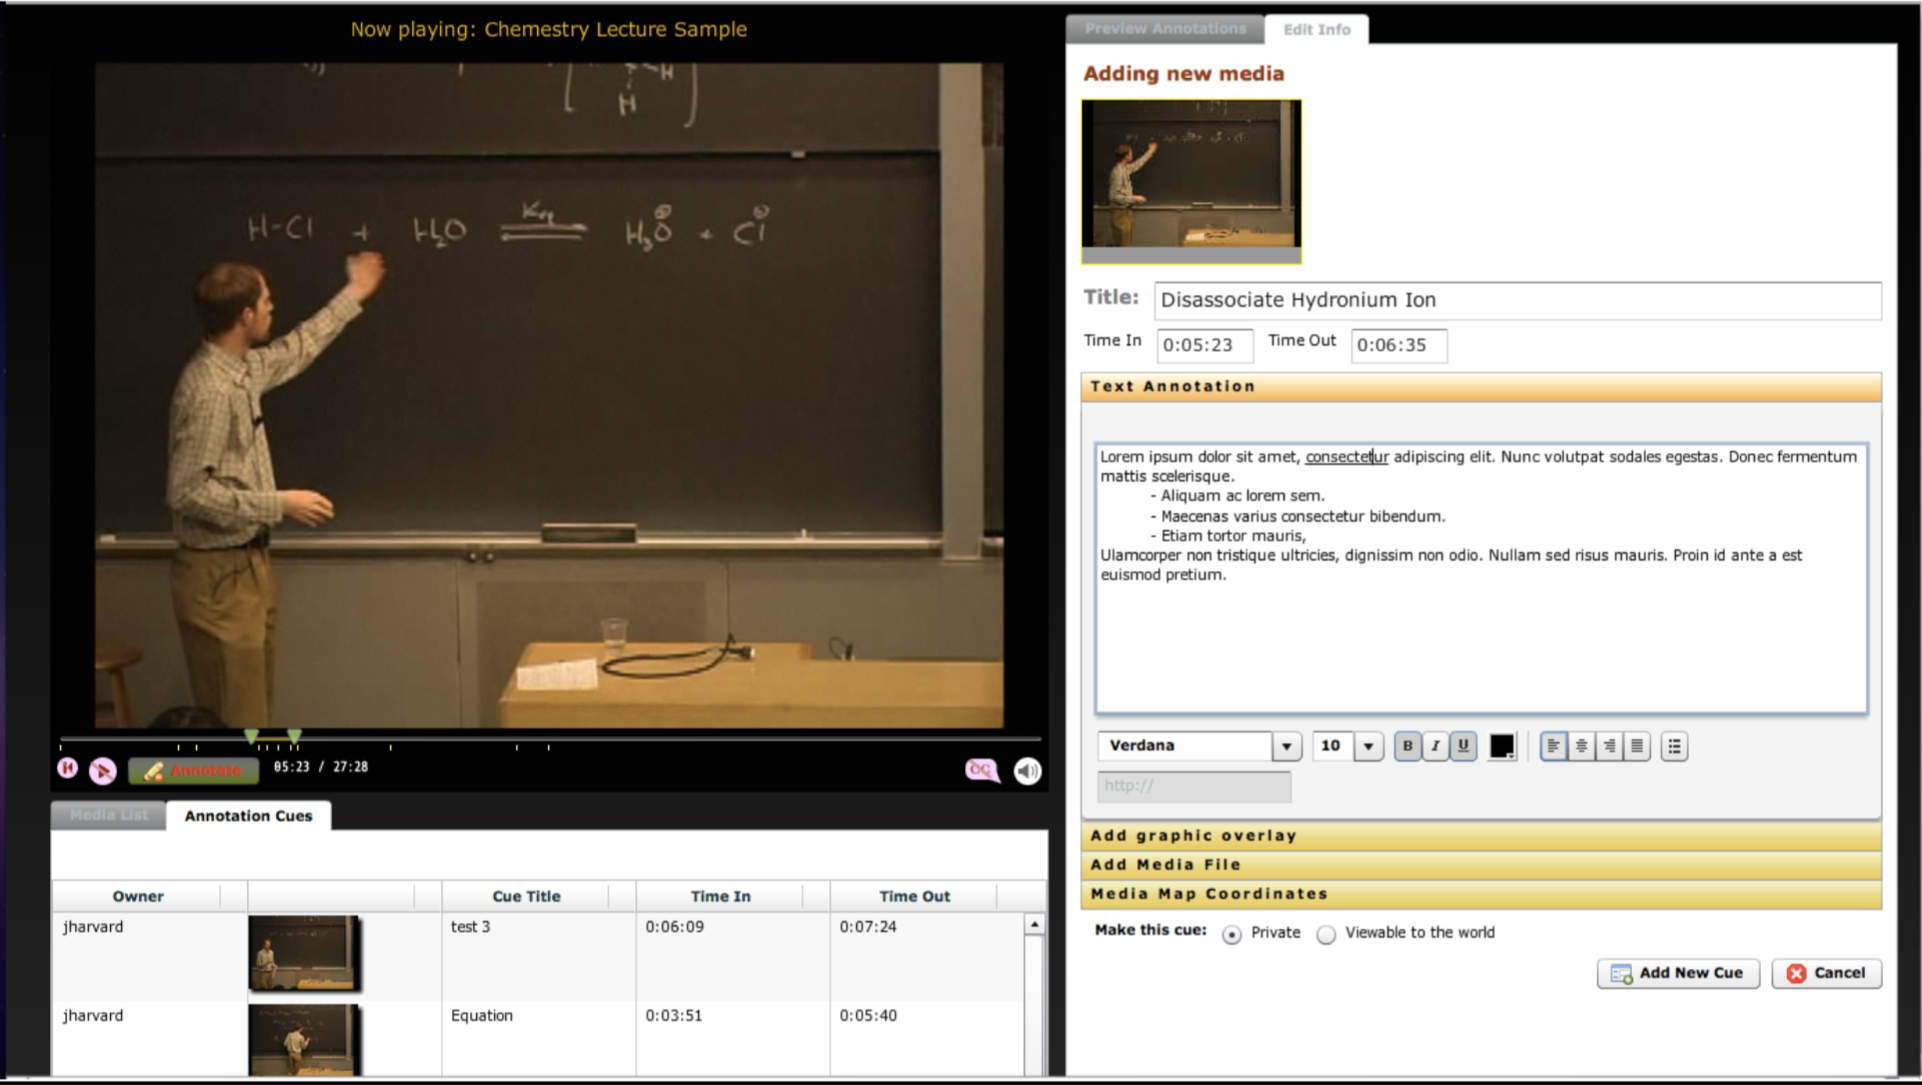
\includegraphics[width=\textwidth]{gfx/mvat/mvat-annotation-edit-view.png}
%	\caption{Figure example: \textit{(a)} example part one, \textit{(c)} example part two; \textit{(c)} example part three} 
%	\label{fig:mvat:example1}
%\end{figure} 
%\begin{figure}[htb]
%	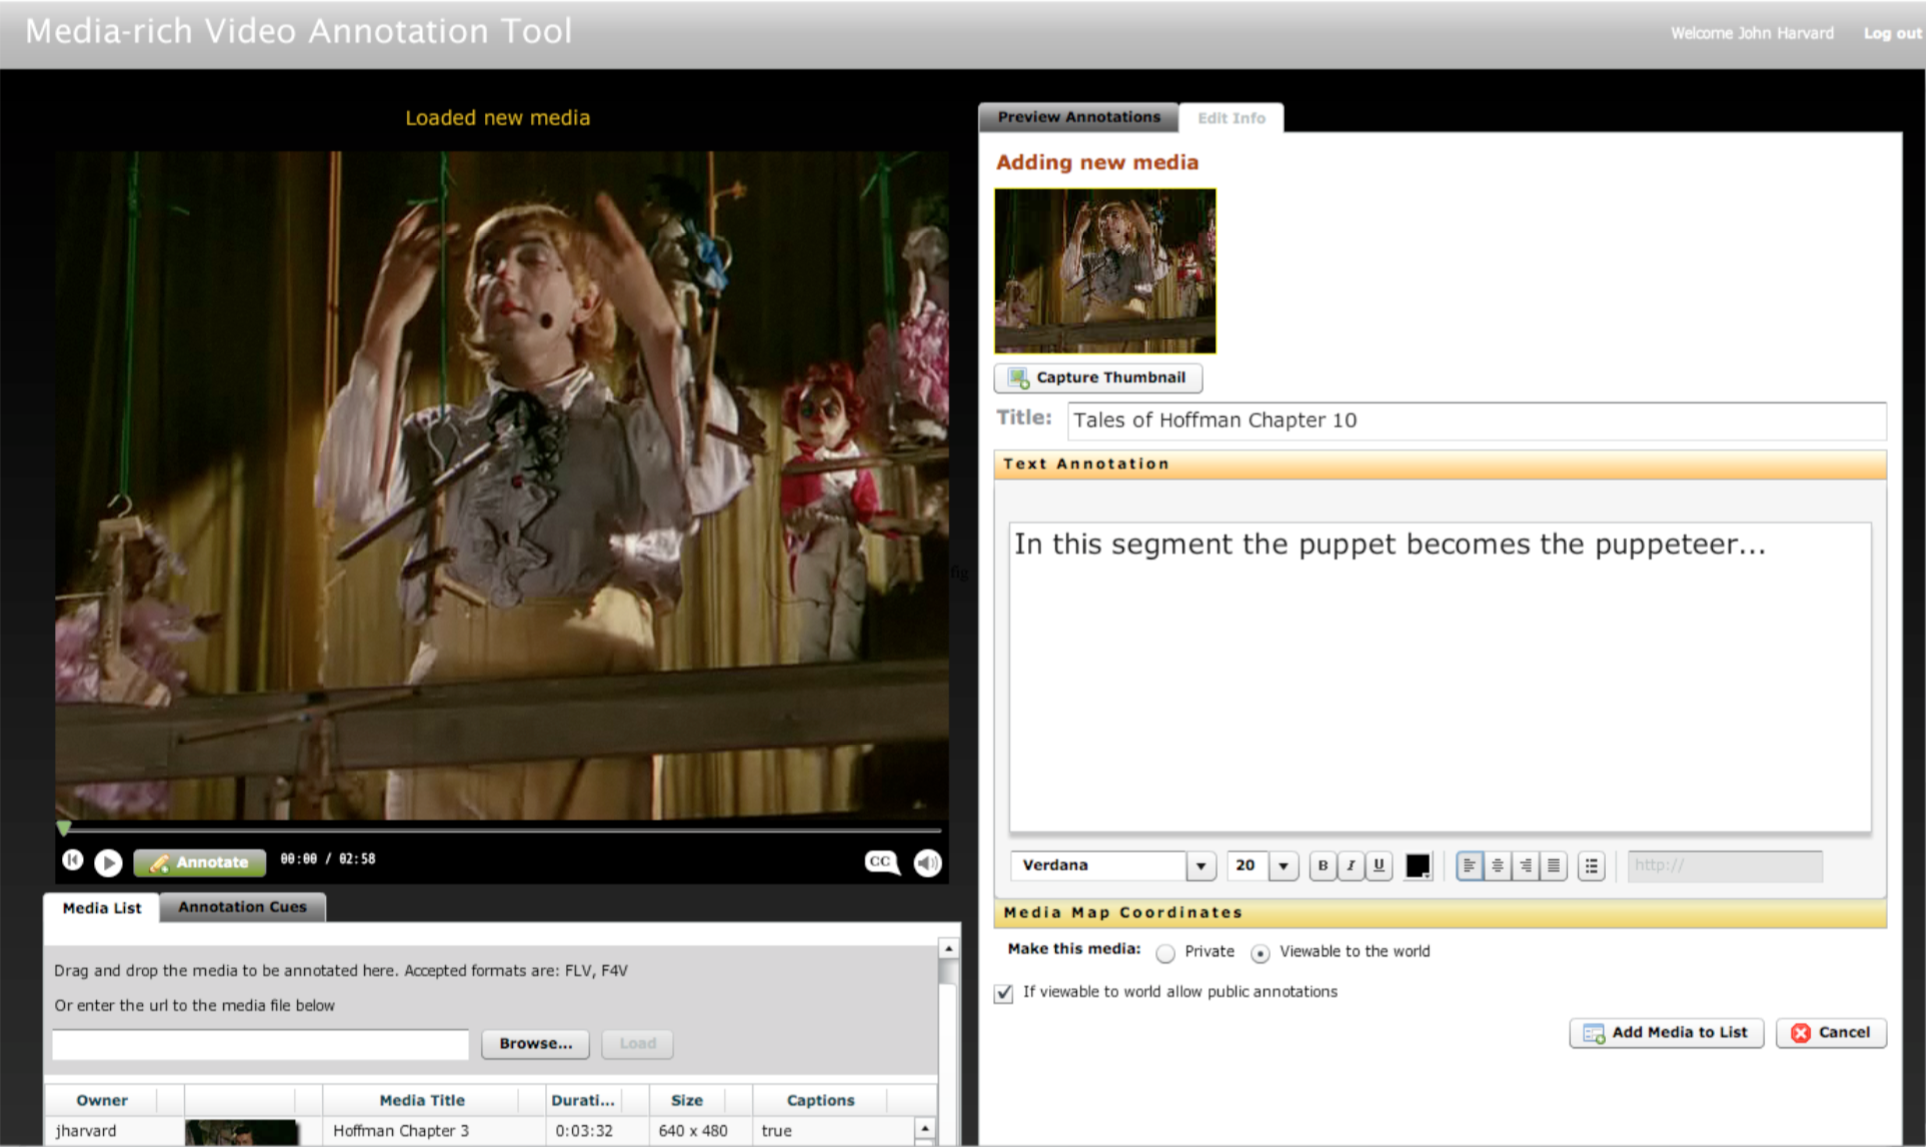
\includegraphics[width=\textwidth]{gfx/mvat/mvat-loading-video-adding-metadata.png}
%	\caption{Figure example: \textit{(a)} example part one, \textit{(c)} example part two; \textit{(c)} example part three} 
%	\label{fig:mvat:example2}
%\end{figure} 
%\begin{figure}[htb]
%	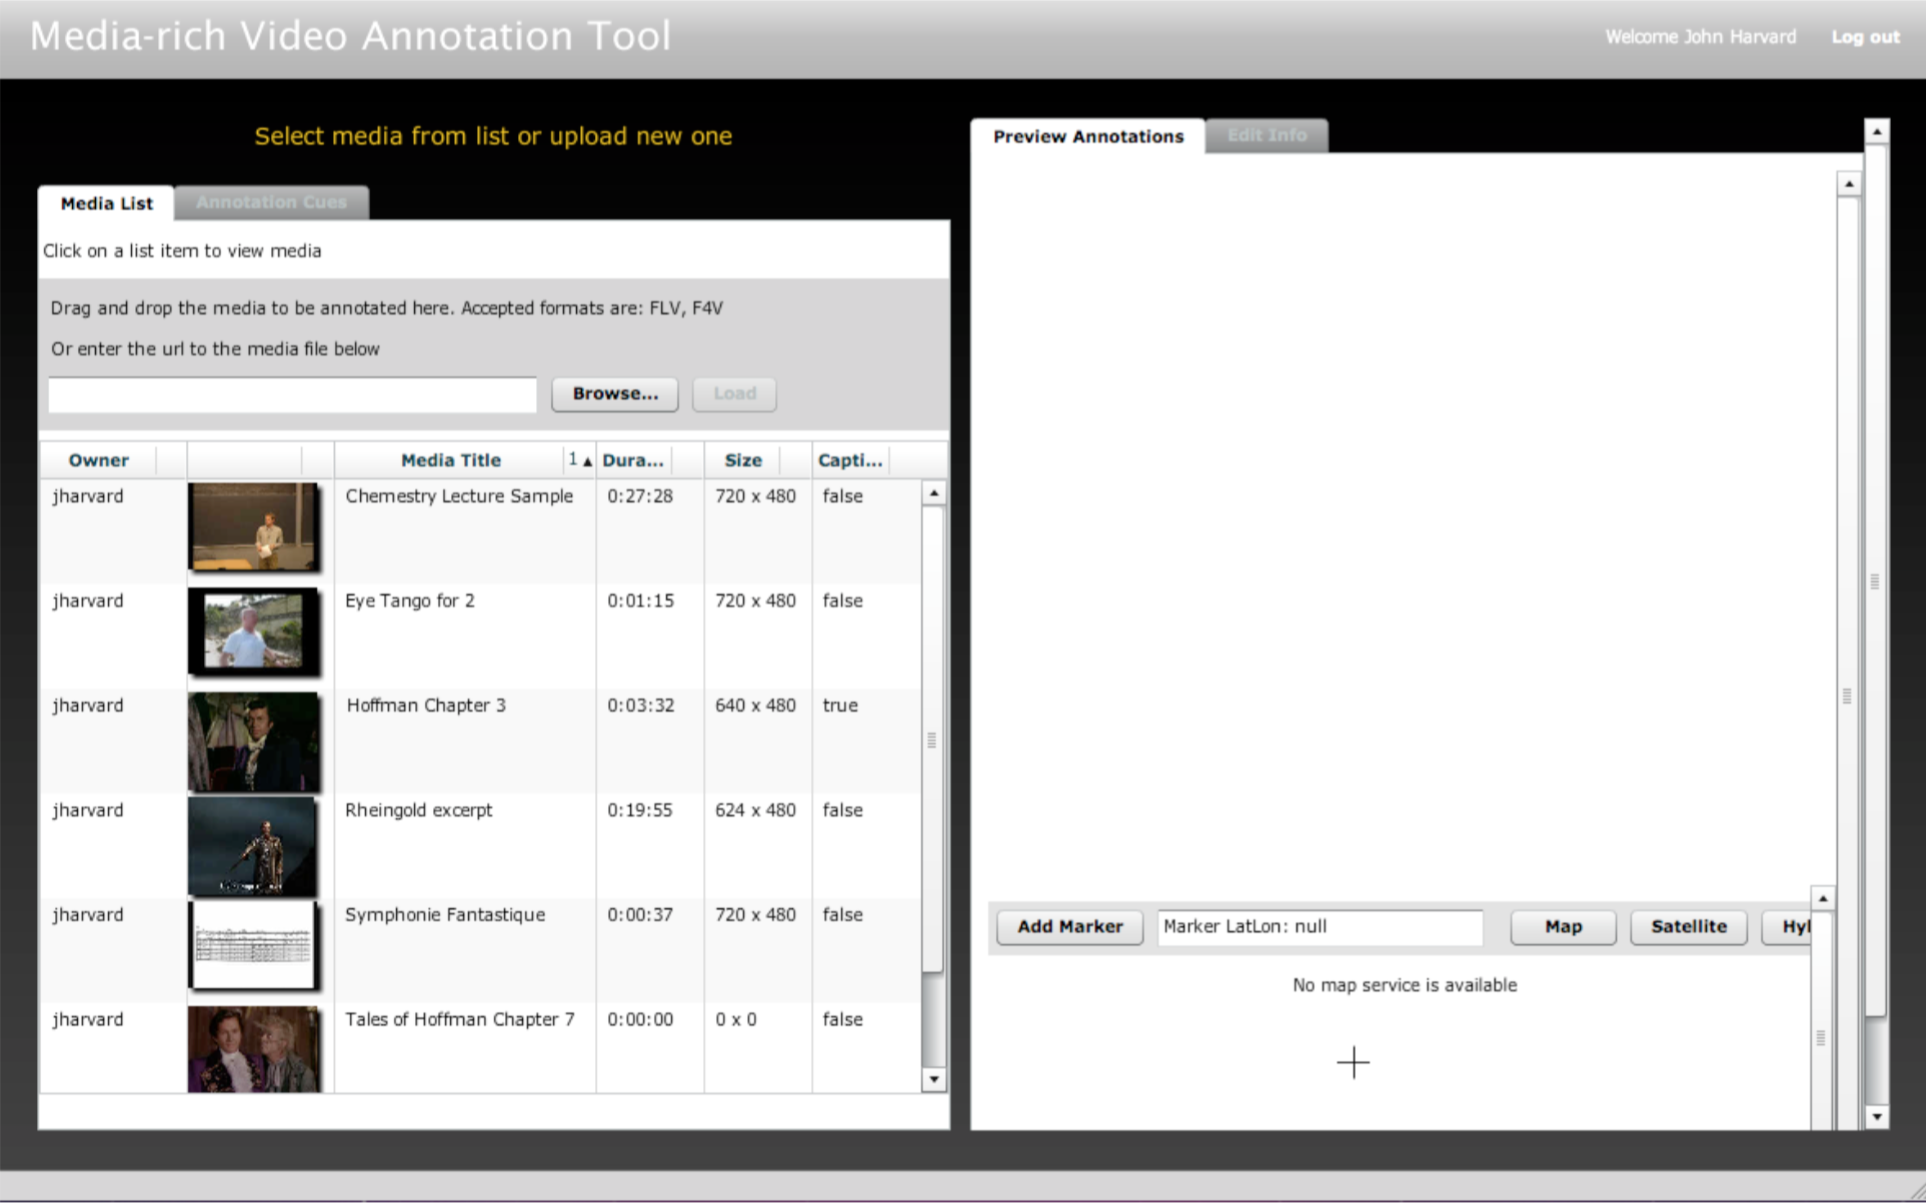
\includegraphics[width=\textwidth]{gfx/mvat/mvat-video-management}
%	\caption{Figure example: \textit{(a)} example part one, \textit{(c)} example part two; \textit{(c)} example part three}
%	\label{fig:mvat:example3}
%\end{figure}



%}

%\begin{figure}[htb]
%	
\includegraphics[width=\textwidth]{gfx/Clean-Thesis-Figure}
%	\caption{Figure example: \textit{(a)} example part one, \textit{(c)} example part two; \textit{(c)} example part three}
%	\label{fig:system:example1}
%\end{figure}
%
%\\ 
%%%%%%%%%%%{\centering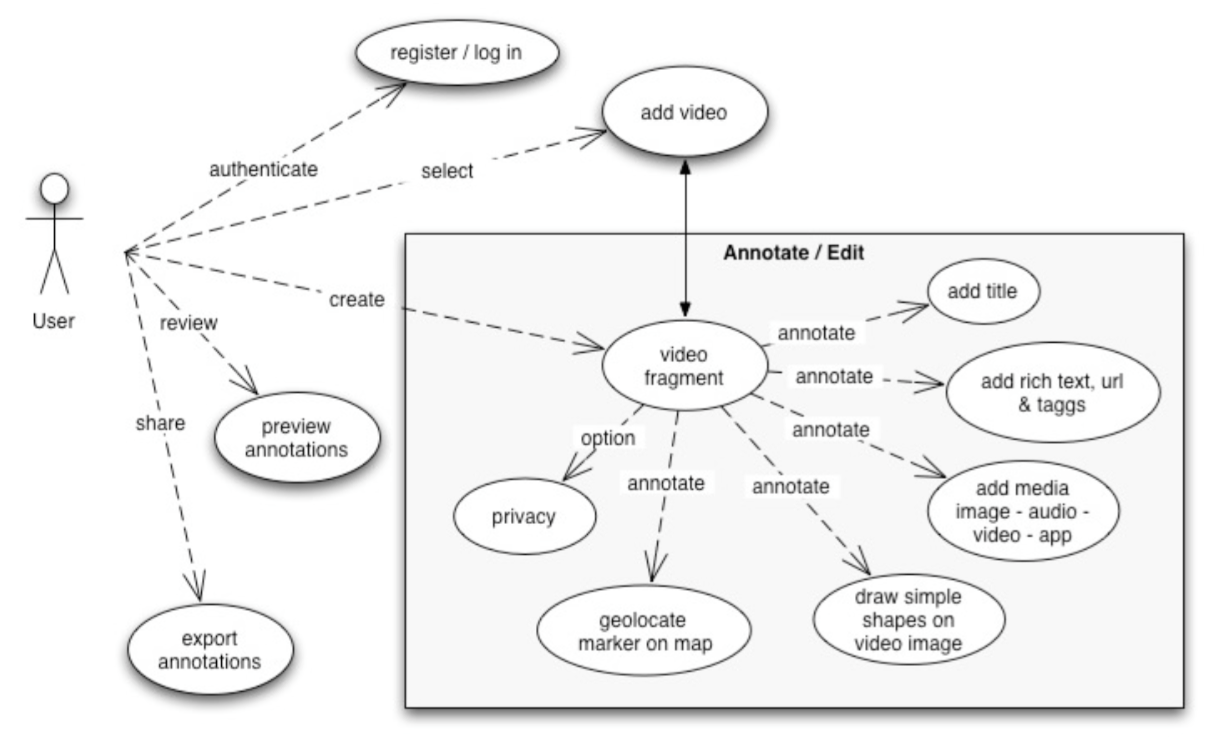
\includegraphics[width=1\textwidth]{gfx/mvat/mvat-core-use-case-diagram.png}} \\
%{\centering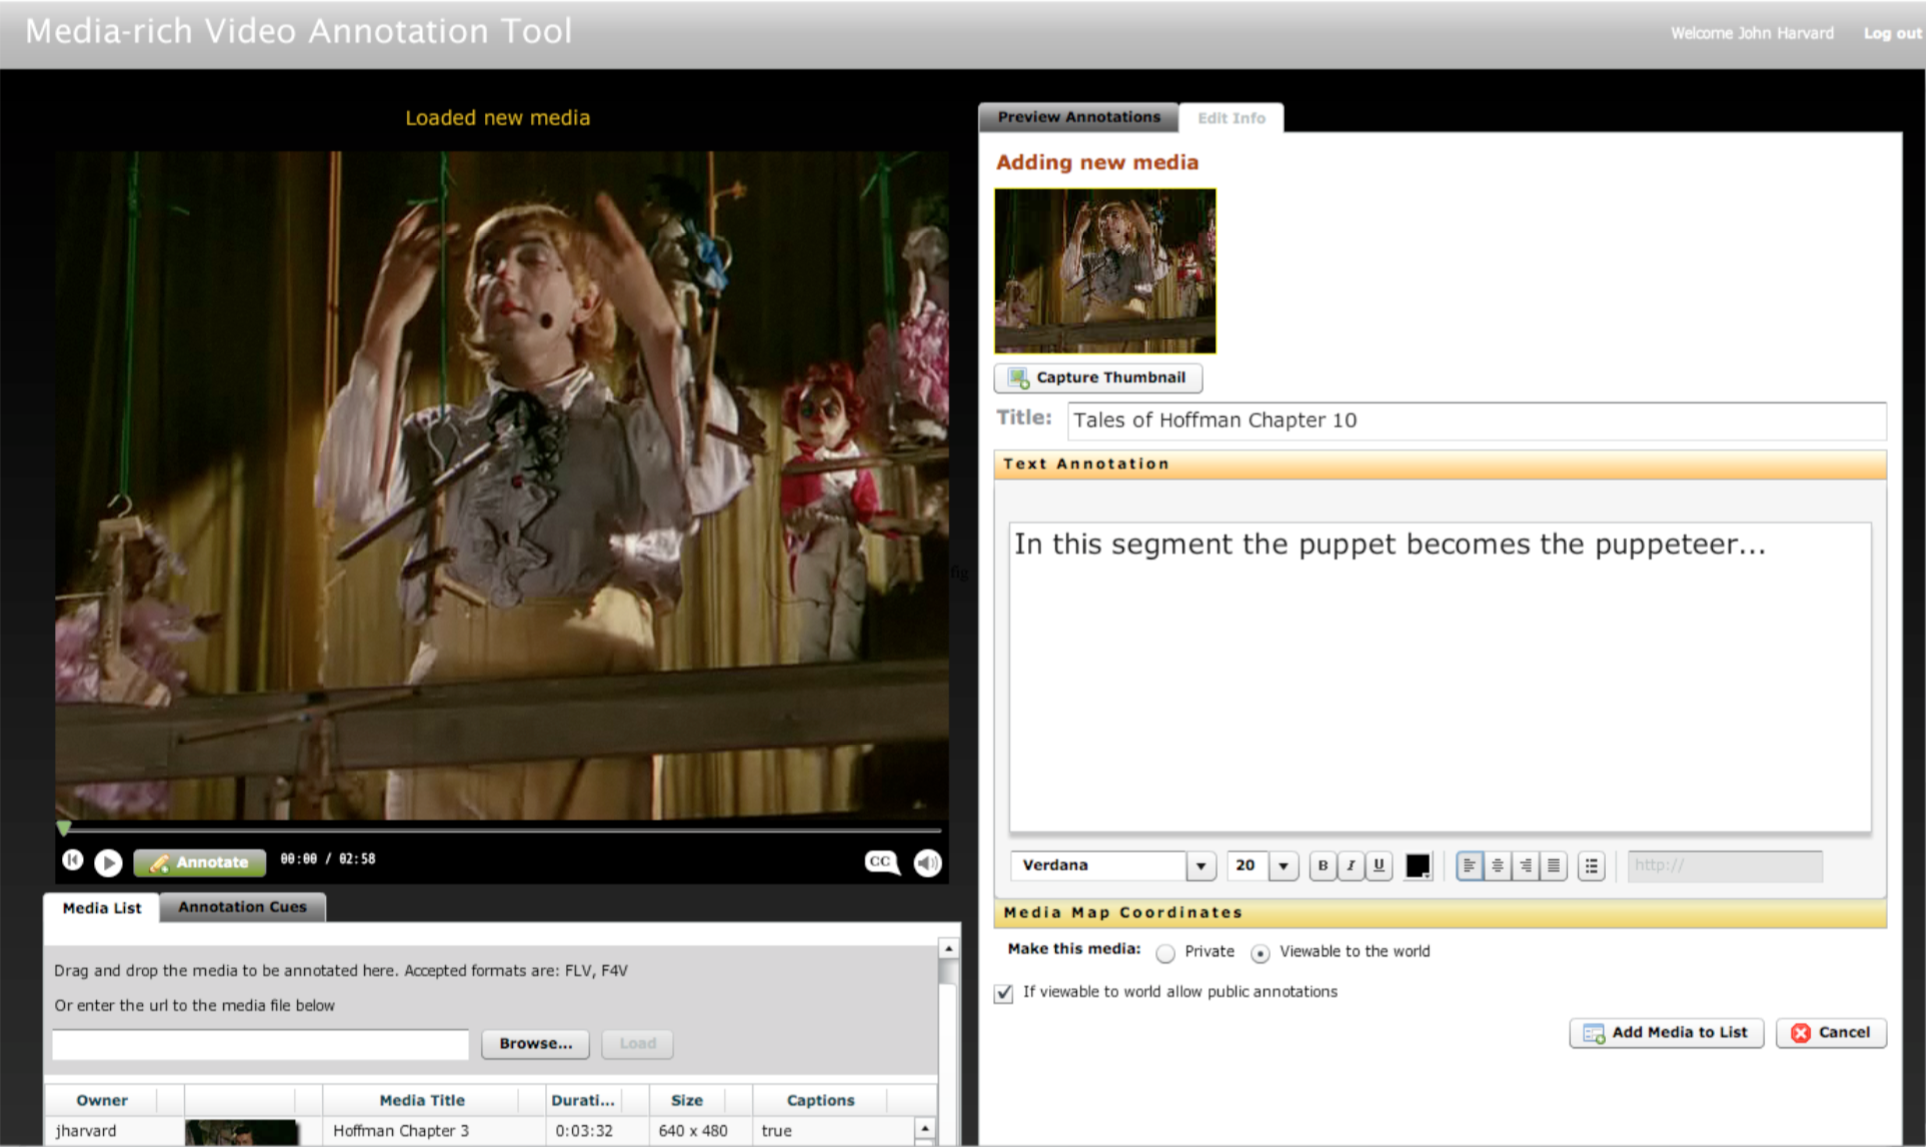
\includegraphics[width=1\textwidth]{gfx/mvat/mvat-loading-video-adding-metadata.png}} \\
%\\ 
%%%%%%%%%%%{\centering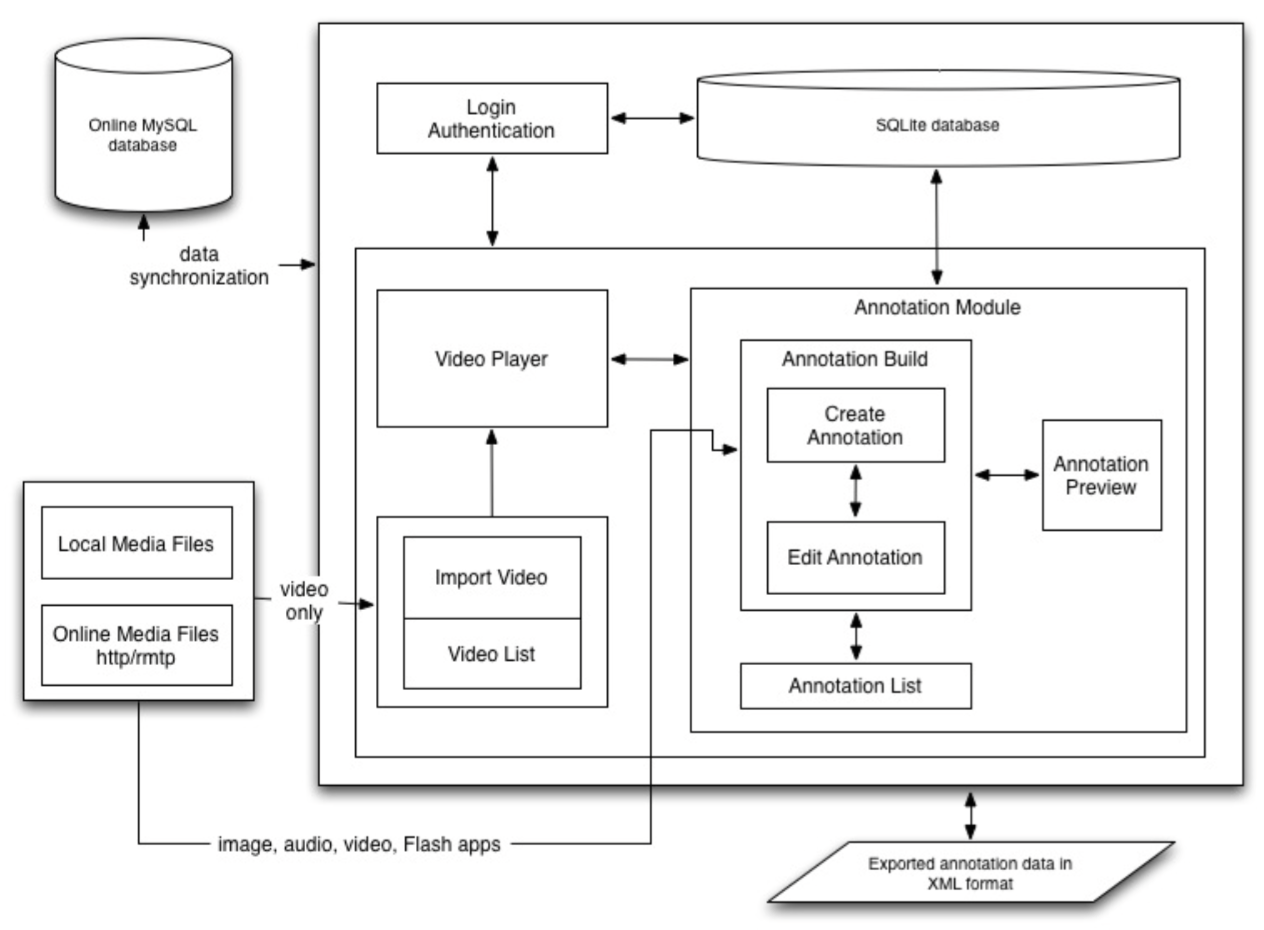
\includegraphics[width=1\textwidth]{gfx/mvat/mvat-system-architecture-overview.png}} \\
%%%%%%%%%%%{\centering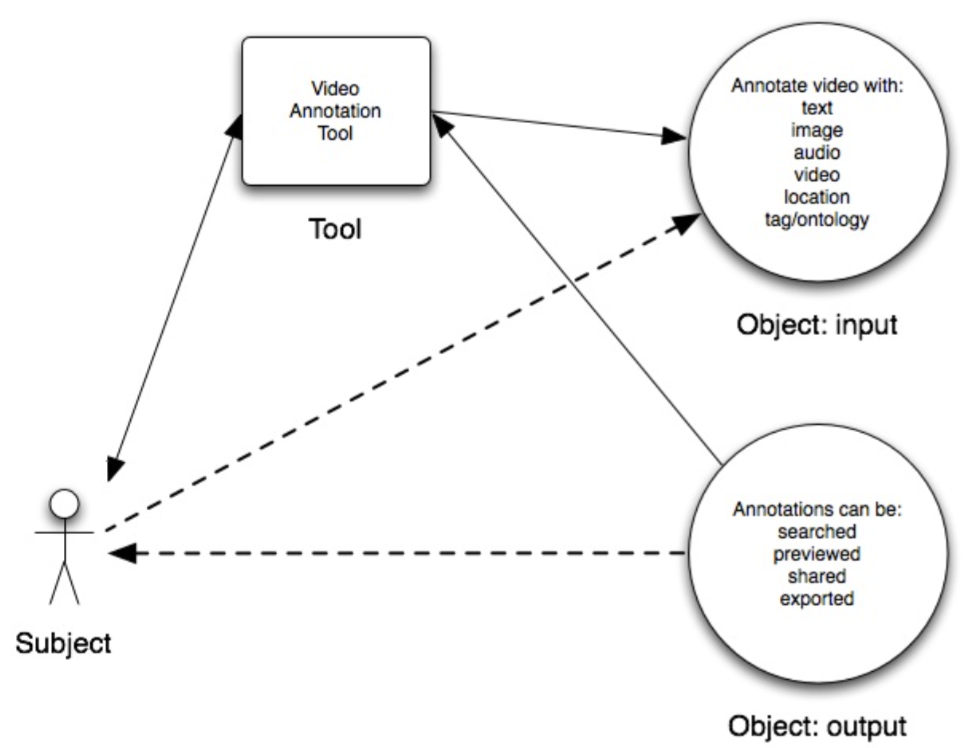
\includegraphics[width=1\textwidth]{gfx/mvat/mvat-use-case-diagram.png}} \\
%{\centering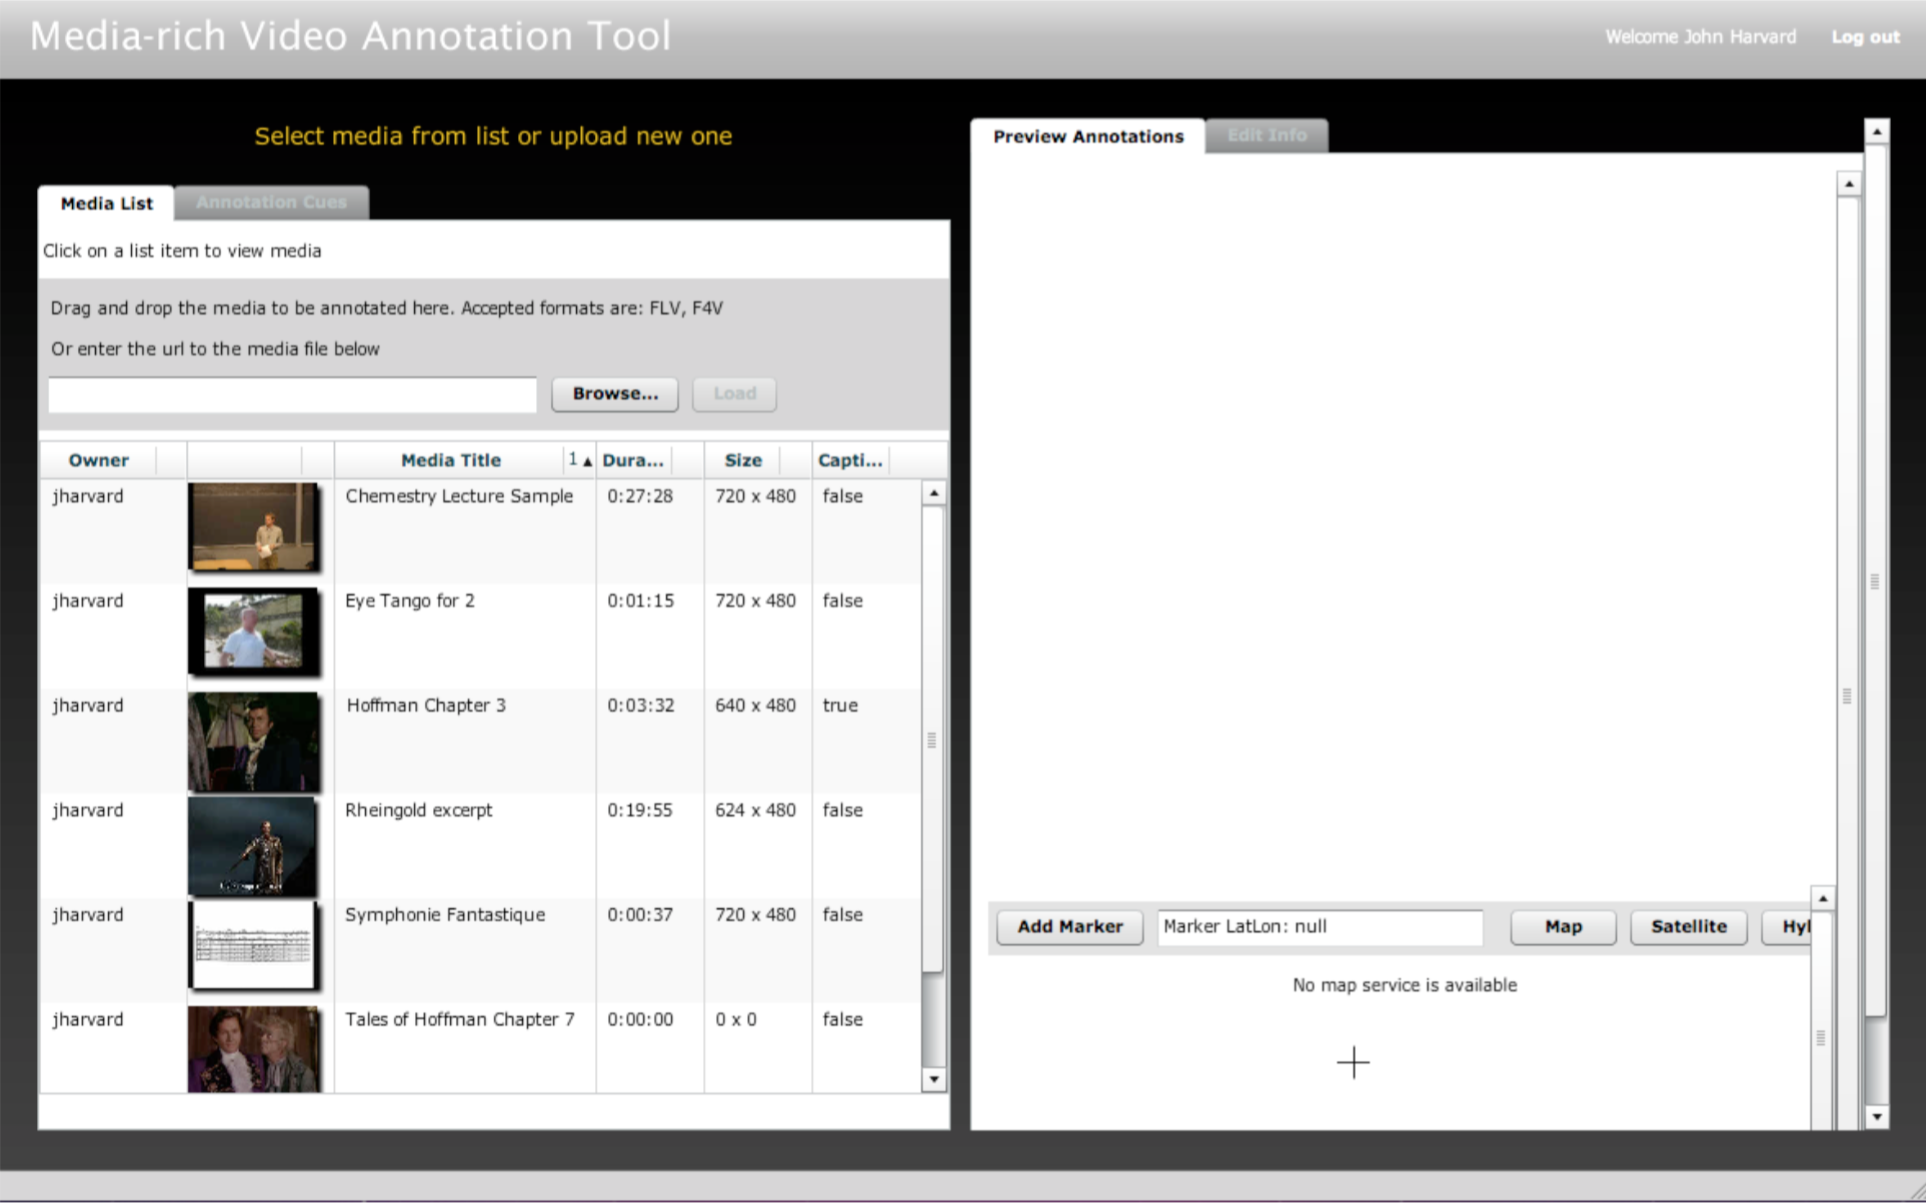
\includegraphics[width=1\textwidth]{gfx/mvat/mvat-video-management.png}} \\
%\\ 


%\href{http://www.people.fas.harvard.edu/~desenne/avac/}
%\href{https://forge.abcd.harvard.edu/gf/project/mvat/}
%\href{http://www.philipdesenne.com}
%\href{http://www.openvideoannotation.org/}

%\item \href{http://phx.corporate-ir.net/phoenix.zhtml?c=176060&p=irol-newsArticle&ID=2034369}{Amazon X-Ray}, by Amazon.com, Inc



\section{Amazon X-Ray}
\label{sec:priorwork:amazon-x-ray}
%\href{http://phx.corporate-ir.net/phoenix.zhtml?c=176060&p=irol-newsArticle&ID=2034369}{Amazon X-Ray}, by Amazon.com, Inc. \\
\textit{by Amazon.com, Inc.}

\begin{figure}[ht]
	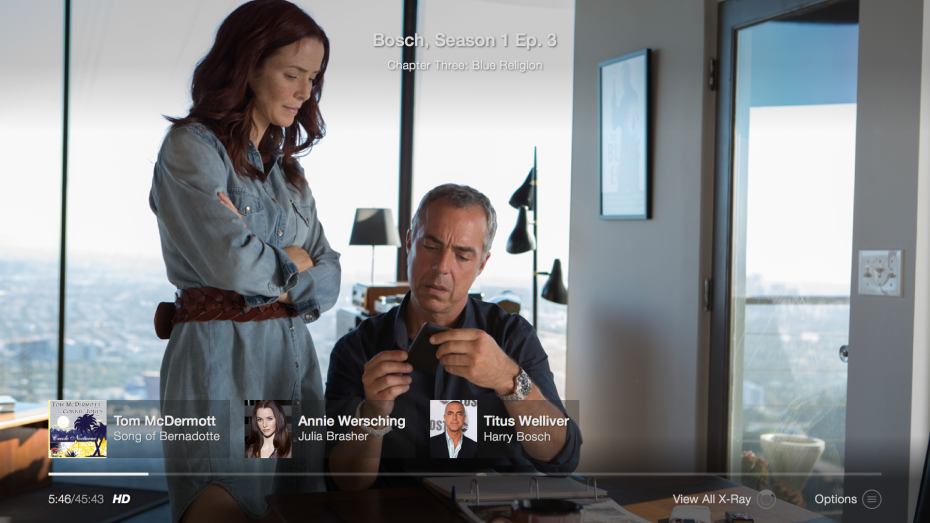
\includegraphics[width=\textwidth]{gfx/amazon-x-ray/pause-quick-view-930x523.png}
	\caption{\textit{(Amazon X-Ray)} pausing a video displays relevant annotations and links to \href{http://www.imdb.com}{IMDB}} 
	\label{fig:amazon-x-ray:paused-video-annotations}
\end{figure} 

\begin{figure}[ht]
	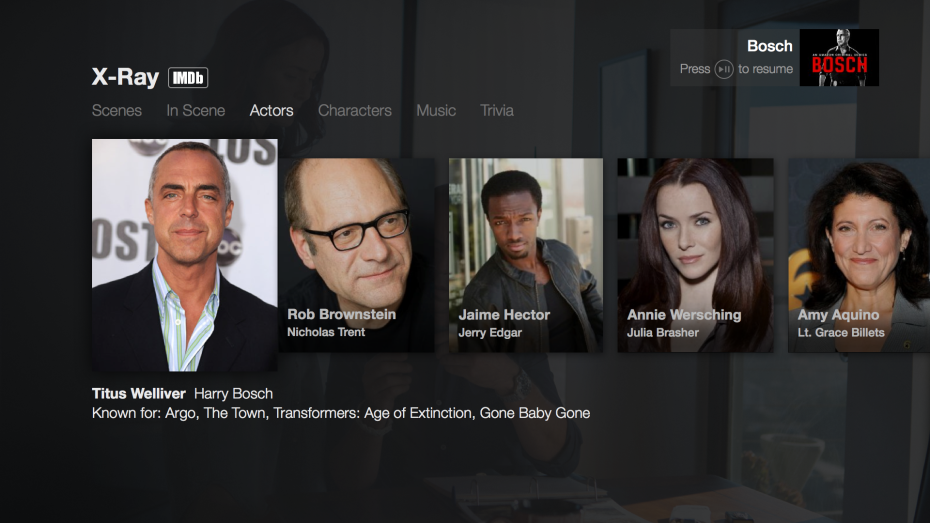
\includegraphics[width=\textwidth]{gfx/amazon-x-ray/xray-actors-930x523.png}
	\caption{\textit{(Amazon X-Ray)} displaying an annotation of all main actors in a film, linking to individual actor profiles on \href{http://www.imdb.com}{IMDB}} 
	\label{fig:amazon-x-ray:actors-listing}
\end{figure}

Amazon has developed a technology that is now being used in several of their video players, from HTML5 enabled web browsers, to portable devices such as the Kindle Fire, and to the Amazon Fire TV sticks. X-Ray presents a video overlay on top of a video as it is playing (or on some devices, when a video is paused) and shows relevant metadata such as the actors that are currently appearing onscreen (and links to their IMDB webpages), the director(s), links to artists whose music is currently playing, etc.  One of the motivating factors for the development of X-Ray for Amazon was to allow viewers to answer questions such as \textit{"Who's that guy?", "What's she been in?", or "What is that song?"} (see \url{http://www.businesswire.com/multimedia/home/20150413005383/en/}). 

The metadata that is used to power these real-time annotations comes from the \href{http://www.imdb.com/x-ray/}{Internet Movie Database}, which is an Amazon owned property.  Unfortunately there is not much in the way of technical details on the underlying technology or architecture of Amazon X-Ray, so it is difficult to find out how Amazon has created and implemented this technology, and how the metadata that powers the annotations is created (viewing an Amazon Prime hosted video in a web browser, for example, show you these annotations when you mouseover the player windown, and the annotations change as characters move in and out of screen, when a new song begins and ends, etc.).

For more information on Amazon X-Ray, see: 

\begin{itemize}
\item \url{http://www.imdb.com/x-ray/}
\item \url{http://www.businesswire.com/multimedia/home/20150413005383/en/}
\item \url{http://phx.corporate-ir.net/phoenix.zhtml?c=176060&p=irol-newsArticle&ID=2034369}
\item \url{http://www.engadget.com/2012/09/06/amazon-announces-x-ray-for-movies-a-kindle-feature-that-uses-im/}
\item \url{http://venturebeat.com/2015/04/13/amazons-x-ray-arrives-for-fire-tv-and-fire-tv-stick-bringing-context-to-instant-video-on-the-big-screen/}
\item \url{http://www.wired.com/2015/04/amazon-xray-fire-tv/}
\item \url{http://gizmodo.com/5941067/amazons-x-ray-for-movies-knows-what-youre-watchingand-whos-in-it}
\end{itemize}


%\end{enumerate}


%\section{Prior Work Section 1}
%\label{sec:priorwork:sec1}

%\section{Prior Work Section 2}
%\label{sec:priorwork:sec2}

%\section{Prior Work Section 3}
%\label{sec:priorwork:sec3}


\section{Prior Work: Conclusion}
\label{sec:priorwork:conclusion}

There has been some very interesting and promising scholarly work done in the area of video annotations previously, but this thesis project has several unique aspects that it attempts to add and extend off of such prior work to make this project novel. Prior work does not appear to have focused too much on the search aspects of annotations that area created or the discoverability of videos that users might not have otherwise ever seen or known about were the annotations not present.  Social sharing aspects of prior work in the area of video annoation seems to be a missing aspect of much prior work as well.  A large part of the impetus for this project is the acknowledgement that the user in posession of a recording may themselves not know enough to properly annotate the video, but knows others (in this particular case, family members, but the same logic could easily apply to friends, colleagues, classmates, etc.) that would be able to add correct annotations.

%\Blindtext[2][1]
        % INCLUDE: related work
% !TEX root = ../dkilleffer-thesis-proposal.tex
%
\chapter{Requirements}
\label{sec:requirements}

\section{Overview}
\label{sec:requirements:overview}

The Social Video platform prototype will allow for users to upload videos, define groups of individuals that are invited to annotate that video, create actual annotations on videos, enable administrators to "approve" annotations prior to those annotations being made public and searchable, and provide a rich, faceted search interface to find and locate videos of interest.

\section{Details}
\label{sec:requirements:details}

Detailed requirements for the prototype are as follows:

%\begin{itemize}[noitemsep]
\begin{itemize}[leftmargin=*]
\item \textbf{User Authentication and Authorization} \\
	New users may create an account and request a particular level of access (\textbf{Regular User} or \textbf{Administrative User}).  \textbf{Regular Users} are allowed to annotate videos, but \textbf{Administrative Users} can upload videos, create annotations, and "approve" annotations that \textbf{Regular Users} have added prior to those being made public and searchable.
\item \textbf{User-Defined Groups} \\

\item \textbf{Rich Annotations} \\

\item \textbf{Video Upload} \\
	
\item \textbf{Faceted Search} \\

\item \textbf{Video Playlists} \\

\end{itemize}



\section{Technologies Used}
\label{sec:requirements:technologies-used}

In contrast to some earlier work, a key goal of this prototype is for the tool to be a purely online system, allowing for web-based collaboration between users.  



%\cleanchapterquote{Innovation distinguishes between a leader and a follower.}{Steve Jobs}{(CEO Apple Inc.)}
%
%\Blindtext[2][1]
%
%\section{Requirements Section 1}
%\label{sec:requirements:sec1}
%
%\Blindtext[1][2]
%
%\begin{figure}[htb]
%	
\includegraphics[width=\textwidth]{gfx/Clean-Thesis-Figure}
%	\caption{Figure example: \textit{(a)} example part one, \textit{(c)} example part two; \textit{(c)} example part three}
%	\label{fig:requirements:example1}
%\end{figure}
%
%\Blindtext[1][2]

%\section{Requirements Section 2}
%\label{sec:requirements:sec2}
%
%\Blindtext[1][2]

%\begin{figure}[htb]
%	
\includegraphics[width=\textwidth]{gfx/Clean-Thesis-Figure}
%	\caption{Another Figure example: \textit{(a)} example part one, \textit{(c)} example part two; \textit{(c)} example part three}
%	\label{fig:requirements:example2}
%\end{figure}
%
%\Blindtext[2][2]

%\section{Requirements Section 3}
%\label{sec:requirements:sec3}
%
%\Blindtext[4][2]

%\section{Conclusion}
%\label{sec:requirements:conclusion}
%
%\Blindtext[2][1]
	  % INCLUDE: requirements
% !TEX root = ../dkilleffer-thesis-proposal.tex
%
\chapter{System}
\label{sec:system}

%\cleanchapterquote{Innovation distinguishes between a leader and a follower.}{Steve Jobs}{(CEO Apple Inc.)}
%
%\Blindtext[2][1]
%
%\section{System Section 1}
%\label{sec:system:sec1}
%
%\Blindtext[1][2]
%
%\begin{figure}[htb]
%	
\includegraphics[width=\textwidth]{gfx/Clean-Thesis-Figure}
%	\caption{Figure example: \textit{(a)} example part one, \textit{(c)} example part two; \textit{(c)} example part three}
%	\label{fig:system:example1}
%\end{figure}
%
%\Blindtext[1][2]
%
%\section{System Section 2}
%\label{sec:system:sec2}
%
%\Blindtext[1][2]
%
%\begin{figure}[htb]
%	
\includegraphics[width=\textwidth]{gfx/Clean-Thesis-Figure}
%	\caption{Another Figure example: \textit{(a)} example part one, \textit{(c)} example part two; \textit{(c)} example part three}
%	\label{fig:system:example2}
%\end{figure}
%
%\Blindtext[2][2]
%
%\section{System Section 3}
%\label{sec:system:sec3}
%
%\Blindtext[4][2]
%
%\section{Conclusion}
%\label{sec:system:conclusion}
%
%\Blindtext[2][1]
	          % INCLUDE: system
% !TEX root = ../dkilleffer-thesis-proposal.tex
%
\chapter{Design}
\label{sec:design}


\section{Overview}
\label{sec:design:overview}

%\Blindtext[1][2]


\section{Technologies Used}
\label{sec:overview:technologies-used}

In contrast to some earlier work, a key goal of this prototype is for the tool to be a purely online system, allowing for web-based collaboration between users.  

%\cleanchapterquote{Innovation distinguishes between a leader and a follower.}{Steve Jobs}{(CEO Apple Inc.)}
%
%\Blindtext[2][1]
%
%\section{Design Section 1}
%\label{sec:design:sec1}
%
%\Blindtext[1][2]
%
%\begin{figure}[htb]
%	
\includegraphics[width=\textwidth]{gfx/Clean-Thesis-Figure}
%	\caption{Figure example: \textit{(a)} example part one, \textit{(c)} example part two; \textit{(c)} example part three}
%	\label{fig:design:example1}
%\end{figure}
%
%\Blindtext[1][2]
%
%\section{Design Section 2}
%\label{sec:design:sec2}
%
%\Blindtext[1][2]
%
%\begin{figure}[htb]
%	
\includegraphics[width=\textwidth]{gfx/Clean-Thesis-Figure}
%	\caption{Another Figure example: \textit{(a)} example part one, \textit{(c)} example part two; \textit{(c)} example part three}
%	\label{fig:design:example2}
%\end{figure}
%
%\Blindtext[2][2]
%
%\section{Design Section 3}
%\label{sec:design:sec3}
%
%\Blindtext[4][2]
%
%\section{Conclusion}
%\label{sec:design:conclusion}
%
%\Blindtext[2][1]
	          % INCLUDE: design

%%%
%%% TODO: include the sections below in the main thesis, but probably not in the proposal
%%%
%% !TEX root = ../dkilleffer-thesis-proposal.tex
%
\chapter{Algorithms}
\label{sec:algorithms}

\cleanchapterquote{You can’t do better design with a computer, but you can speed up your work enormously.}{Wim Crouwel}{(Graphic designer and typographer)}

\Blindtext[2][2]

\section{Postcards: My Address}
\label{sec:algorithms:address}

\textbf{Ricardo Langner} \\
Alfred-Schrapel-Str. 7 \\
01307 Dresden \\
Germany


\section{Motivation and Problem Statement}
\label{sec:algorithms:motivation}

\Blindtext[3][1] \cite{Jurgens:2000,Jurgens:1995,Miede:2011,Kohm:2011,Apple:keynote:2010,Apple:numbers:2010,Apple:pages:2010}

\section{Results}
\label{sec:algorithms:results}

\Blindtext[1][2]

\subsection{Some References}
\label{sec:algorithms:results:refs}
\cite{WEB:GNU:GPL:2010,WEB:Miede:2011}

\section{Thesis Structure}
\label{sec:algorithms:structure}

\textbf{Chapter \ref{sec:related}} \\[0.2em]
\blindtext

\textbf{Chapter \ref{sec:system}} \\[0.2em]
\blindtext

\textbf{Chapter \ref{sec:concepts}} \\[0.2em]
\blindtext

\textbf{Chapter \ref{sec:concepts}} \\[0.2em]
\blindtext

\textbf{Chapter \ref{sec:conclusion}} \\[0.2em]
\blindtext
	        % INCLUDE: algorithmic challenges
%% !TEX root = ../dkilleffer-thesis-proposal.tex
%
\chapter{Implementation}
\label{sec:implementation}

\cleanchapterquote{You can’t do better design with a computer, but you can speed up your work enormously.}{Wim Crouwel}{(Graphic designer and typographer)}

\Blindtext[2][2]

\section{Postcards: My Address}
\label{sec:implementation:address}

\textbf{Ricardo Langner} \\
Alfred-Schrapel-Str. 7 \\
01307 Dresden \\
Germany


\section{Motivation and Problem Statement}
\label{sec:implementation:motivation}

\Blindtext[3][1] \cite{Jurgens:2000,Jurgens:1995,Miede:2011,Kohm:2011,Apple:keynote:2010,Apple:numbers:2010,Apple:pages:2010}

\section{Results}
\label{sec:implementation:results}

\Blindtext[1][2]

\subsection{Implementation References}
\label{sec:implementation:results:refs}
\cite{WEB:GNU:GPL:2010,WEB:Miede:2011}

\section{Implementation Structure}
\label{sec:implementation:structure}

\textbf{Chapter \ref{sec:related}} \\[0.2em]
\blindtext

\textbf{Chapter \ref{sec:system}} \\[0.2em]
\blindtext

\textbf{Chapter \ref{sec:concepts}} \\[0.2em]
\blindtext

\textbf{Chapter \ref{sec:concepts}} \\[0.2em]
\blindtext

\textbf{Chapter \ref{sec:conclusion}} \\[0.2em]
\blindtext
	    % INCLUDE: implementation analysis
%% !TEX root = ../dkilleffer-thesis-proposal.tex
%
\chapter{User Guide}
\label{sec:userguide}

\cleanchapterquote{A picture is worth a thousand words. An interface is worth a thousand pictures.}{Ben Shneiderman}{(Professor for Computer Science)}

\Blindtext[2][1]

\section{User Guide Section 1}
\label{sec:userguide:sec1}

\Blindtext[2][2]

\section{User Guide Section 2}
\label{sec:userguide:sec2}

\Blindtext[3][2]

\section{User Guide Section 3}
\label{sec:userguide:sec3}

\Blindtext[4][2]

\section{User Guide Conclusion}
\label{sec:userguide:conclusion}

\Blindtext[2][1]
	        % INCLUDE: user guide
%% !TEX root = ../dkilleffer-thesis-proposal.tex
%
\chapter{Results and Evaluation}
\label{sec:results}

\cleanchapterquote{A picture is worth a thousand words. An interface is worth a thousand pictures.}{Ben Shneiderman}{(Professor for Computer Science)}

\Blindtext[2][1]

\section{Results Section 1}
\label{sec:related:sec1}

\Blindtext[2][2]

\section{Results Section 2}
\label{sec:results:sec2}

\Blindtext[3][2]

\section{Results Section 3}
\label{sec:results:sec3}

\Blindtext[4][2]

\section{Results Conclusion}
\label{sec:results:conclusion}

\Blindtext[2][1]
	        % INCLUDE: results and evaluation

% !TEX root = ../dkilleffer-thesis-proposal.tex
%
\chapter{Work Plan}
\label{sec:workplan}

%In this chapter, describe what your overall work plan is.  Be as specific as you can as to how the parts of your project work will come together so that you and your thesis director can make better decisions about changes as new information comes to light.

My plan for the development of this project will be to follow a loosely based "Scrum" development methodology, where I attempt to adhere to 2-week "sprints" wherein I successfully complete discrete functional parts of the project, and break out larger funtionality into small chunks that can be built and completed in the shorter sprint timeframe.  Before investing in much of the actual coding portion of the project, I will be developing wireframes that visually indicate the proposed "look and feel" of a prticular webpage.

	        % INCLUDE: work plan
% !TEX root = ../dkilleffer-thesis-proposal.tex
%
\chapter{Risks and Alternatives}
\label{sec:risksandalternatives}



%Describe the development environment you require (language, OS, system) and other tools you expect to use.  Also describe any assumptions you have made about what it will take to finish your work.

%Describe the risks you now see as inherent in your work and alternatives you might have to take to ameliorate these risks (e.g., project scope and alternatives for scope reduction)



%\section{Risks and Alternatives Section 1}
%\label{sec:risksandalternatives:sec1}
%
%\Blindtext[2][2]
%
%\section{Risks and Alternatives Section 2}
%\label{sec:risksandalternatives:sec2}
%
%\Blindtext[3][2]
%
%\section{Risks and Alternatives Section 3}
%\label{sec:risksandalternatives:sec3}
%
%\Blindtext[4][2]
%
%\section{Risks and Alternatives Conclusion}
%\label{sec:risksandalternatives:conclusion}
%
%\Blindtext[2][1]
  % INCLUDE: risks and alternatives
% !TEX root = ../dkilleffer-thesis-proposal.tex
%
\chapter{Preliminary Schedule}
\label{sec:schedule}


%Give a breakdown of the activities that lead to completion of major milestones in your work, and give rough time estimates for completing these activities.  These should be at the level of detail of 2-4 weeks each.


\begin{table}[ht]
\centering
\begin{tabularx}{\linewidth}{
    |>{\hsize=0.5\hsize}X|% 25% of 2\hsize 
    >{\hsize=1.5\hsize}X|% 75% of 2\hsize
       % sum=2.0\hsize for 2 columns
} \hline
 \textbf{Month/Year} & \textbf{Description} \\ \hline
\rowcolor{mymagenta1}{July 2016} & {Lorem ipsum dolor sit amet, consectetur adipiscing elit. Fusce at varius ipsum, quis imperdiet dolor. Pellentesque tincidunt massa at felis pulvinar dictum. Nunc viverra euismod odio, vitae aliquet nunc accumsan ut. Aenean mauris purus, lobortis nec rutrum eget, interdum id ipsum. Duis vulputate nisl sed turpis bibendum dignissim. Aenean porttitor suscipit dui, quis elementum lectus ultrices non. Donec ut tincidunt nunc. Vestibulum ultricies diam eget ante fringilla maximus. Duis et congue ligula.

Vestibulum in auctor neque. Duis lobortis consequat enim nec hendrerit. Sed felis dui, tincidunt a sapien ac, elementum iaculis ex. Ut nulla nisl, dictum et mauris eu, condimentum pretium sapien. Donec pulvinar, lectus eu pulvinar rutrum, justo risus laoreet ipsum, nec aliquam sem mi sit amet orci. Morbi scelerisque tempor mi sed pharetra. Maecenas dignissim aliquam convallis. Aliquam sagittis elementum enim, vel dignissim quam porta eu. Vestibulum ullamcorper varius orci, id consectetur massa rutrum commodo. Nunc semper posuere pretium. Aenean molestie vestibulum sapien id mattis. Pellentesque a iaculis dolor. Nulla facilisi. Morbi luctus justo et est porttitor malesuada.} \\ \hline
 \rowcolor{mymagenta2}{August 2016} & {do more work} \\ \hline
 \rowcolor{mymagenta3}{September 2016} & {do more work} \\ \hline
 \rowcolor{mymagenta4}{October 2016}   & {do more work} \\ \hline
 \rowcolor{mymagenta5}{November 2016}  & {do more work} \\ \hline
 \rowcolor{mymagenta6}{December 2016}  & {do more work} \\ \hline
 \rowcolor{mymagenta7}{January 2017}   & {do more work} \\ \hline
 \rowcolor{mymagenta8}{February 2017}  & {do more work} \\ \hline
 \rowcolor{mymagenta9}{March 2017}     & {do more work} \\ \hline
 \rowcolor{mymagenta10}{April 2017}     & {do more work} \\ \hline
 \rowcolor{mymagenta1}{May 2017}       & {last bit of work} \\ \hline 
%\end{tabular}
\end{tabularx}
\caption{Preliminary Project Schedule}
\label{sec:schedule:preliminary-schedule}
\end{table}

            % INCLUDE: preliminary project schedule

%%% !TEX root = ../thesis-example.tex
%
\chapter{Concepts: This text is here to test a very long title, to simulate the line break behavior, to show that an extremely long tilte also works}
\label{sec:concepts}

\cleanchapterquote{Users do not care about what is inside the box, as long as the box does what they need done.}{Jef Raskin}{about Human Computer Interfaces}

\Blindtext[2][1]

\section{Concepts Section 1}
\label{sec:concepts:sec1}

\Blindtext[2][2]

\section{Concepts Section 2}
\label{sec:concepts:sec2}

\Blindtext[3][2]

\section{Concepts Section 3}
\label{sec:concepts:sec3}

\Blindtext[4][2]

\section{Conclusion}
\label{sec:concepts:conclusion}

\Blindtext[2][1]
 % INCLUDE: concepts
\cleardoublepage

% --------------------------
% Back matter
% --------------------------
{%
\setstretch{1.1}
\renewcommand{\bibfont}{\normalfont\small}
\setlength{\biblabelsep}{0pt}
\setlength{\bibitemsep}{0.5\baselineskip plus 0.5\baselineskip}
\printbibliography[nottype=online]
\printbibliography[heading=subbibliography,title={Webseiten},type=online,prefixnumbers={@}]
}
\cleardoublepage

\listoffigures
\cleardoublepage

\listoftables
\cleardoublepage


% !TEX root = ../dkilleffer-thesis-proposal.tex
%
\pagestyle{empty}
\hfill
\pdfbookmark[0]{Glossary}{Glossary}
\section*{Glossary}

%You should not assume that all readers are familiar with the technology or terminology referred to in your thesis proposal.  This section should include definitions of major terms and an explanation of acronyms.

Here are some of the terms used throughout this proposal.

\begin{itemize}[leftmargin=*]
\label{glossary:amazon-x-ray}
\item \textbf{Amazon X-Ray} \\
	a reference tool incorporated into several video players that allows for the display and linking of actors, acresses, directors, and linked data when viewing a movie or television show hosted by Amazon. (see \url{https://en.wikipedia.org/wiki/X-Ray_%28Amazon_Kindle%29}, \url{http://www.amazon.com/gp/help/customer/display.html?nodeId=201423010})

\label{glossary:apache-solr}
\item \textbf{Apache Solr} \\
	TODO
\label{glossary:bootstrap}
\item \textbf{Bootstrap} \\
	TODO
\label{glossary:dvd}
\item \textbf{DVD} \\
	Digital Video Disc
\label{glossary:elasticsearch}
\item \textbf{Elasticsearch} \\
	TODO
\label{glossary:express.js}
\item \textbf{Express.js} \\
	TODO
\label{glossary:faceted-search}
\item \textbf{faceted search} \\
	TODO
\label{glossary:json}
\item \textbf{JSON} \\
	TODO
\label{glossary:node.js}
\item \textbf{Node.js} \\
	TODO
\label{glossary:mini-dv}
\item \textbf{Mini-DV} \\
	a successor to the wildly popular VHS home recording system, Mini-DV is a cassette tape format for video recording. It captures video in a resolution close to that of DVD. (see \url{http://techterms.com/definition/minidv})
\label{glossary:react.js}
\item \textbf{React.js} \\
	TODO
\label{glossary:restful-api}
\item \textbf{RESTful API} \\
	TODO
\label{glossary:vhs}
\item \textbf{VHS} \\
	acronnym for "Video Home System", it is a widely-adopted videocassette recording ( VCR ) technology that was developed by Japan Victor Company (JVC) and put on the market in 1976. It uses magnetic tape 1/2 inch (1.27 cm) in width.  It was extremely popular in the 1980s and 1990s, and declined in use during the early 2000s. (adapted from \url{http://whatis.techtarget.com/definition/VHS-Video-Home-System} and \url{https://en.wikipedia.org/wiki/VHS})
\end{itemize}
            % INCLUDE: glossary of terms
\cleardoublepage


% !TEX root = ../dkilleffer-thesis-proposal.tex
%
\pagestyle{empty}
\hfill
\vfill
\pdfbookmark[0]{Colophon}{Colophon}
\section*{Colophon}

This thesis was typeset with \LaTeXe.
It uses the \textit{Clean Thesis} style developed by Ricardo Langner.
The design of the \textit{Clean Thesis} style is inspired by user guide documents from Apple Inc.

Download the \textit{Clean Thesis} style at \url{http://cleanthesis.der-ric.de/}.

\cleardoublepage

% !TEX root = ../thesis-example.tex
%
%************************************************
% Declaration
%************************************************
\pdfbookmark[0]{Declaration}{Declaration}
\chapter*{Declaration}
\label{sec:declaration}
\thispagestyle{empty}

You can put your declaration here, to declare that you have completed your work solely and only with the help of the references you mentioned.

\bigskip

\noindent\textit{\thesisUniversityCity, \thesisDate}

\smallskip

\begin{flushright}
	\begin{minipage}{5cm}
		\rule{\textwidth}{1pt}
		\centering\thesisName
	\end{minipage}
\end{flushright}

%*****************************************
%*****************************************

\clearpage
\newpage
\mbox{}

% **************************************************
% End of Document CONTENT
% **************************************************
\end{document}
